\chapter{Diseño}

En este capítulo se mostrarán los diagramas \textbf{arquitectónico}, de \textbf{clases} y algunos de \textbf{secuencia} de la aplicación. Siendo los dos últimos generados con la aplicación \textit{Visual Paradigm for UML 13.1 Community Edition} \cite{vpp}.

\section{Arquitectura del software}

El software, escrito en C++, hace uso tanto de la CPU como de la GPU a nivel hardware y usa OpenGL como librería gráfica de bajo nivel.

Se hace uso de la librería gráfica de alto nivel VTK, de Qt como librería para crear la GUI y de Boost para usar sus algoritmos en la gestión de ficheros XML.

\begin{table}[H]
	\begin{center}
		\begin{tabular}{|l|c|c|c|c|}
			\hline
			Librerías de alto nivel  & \multicolumn{2}{c|}{Boost} & VTK        & Qt        \\ \hline
			Librerías de bajo nivel  & \multicolumn{4}{c|}{OpenGL}                         \\ \hline
			Lenguaje de programación & \multicolumn{4}{c|}{C++}                            \\ \hline
			Nivel Hardware           & \multicolumn{2}{c|}{CPU} & \multicolumn{2}{c|}{GPU} \\ \hline
		\end{tabular}
	\end{center}
	\caption{Arquitectura del software}
	\label{tab:diagrama_arquitectonico}
\end{table}

\section{Diagramas de clases}

Se presentan las distintas clases en tres diagramas distintos para ser mostrados con más claridad aunque no estén separados en paquetes como tales.

\subsection{Volume}

\begin{figure}[H]
	\centering
	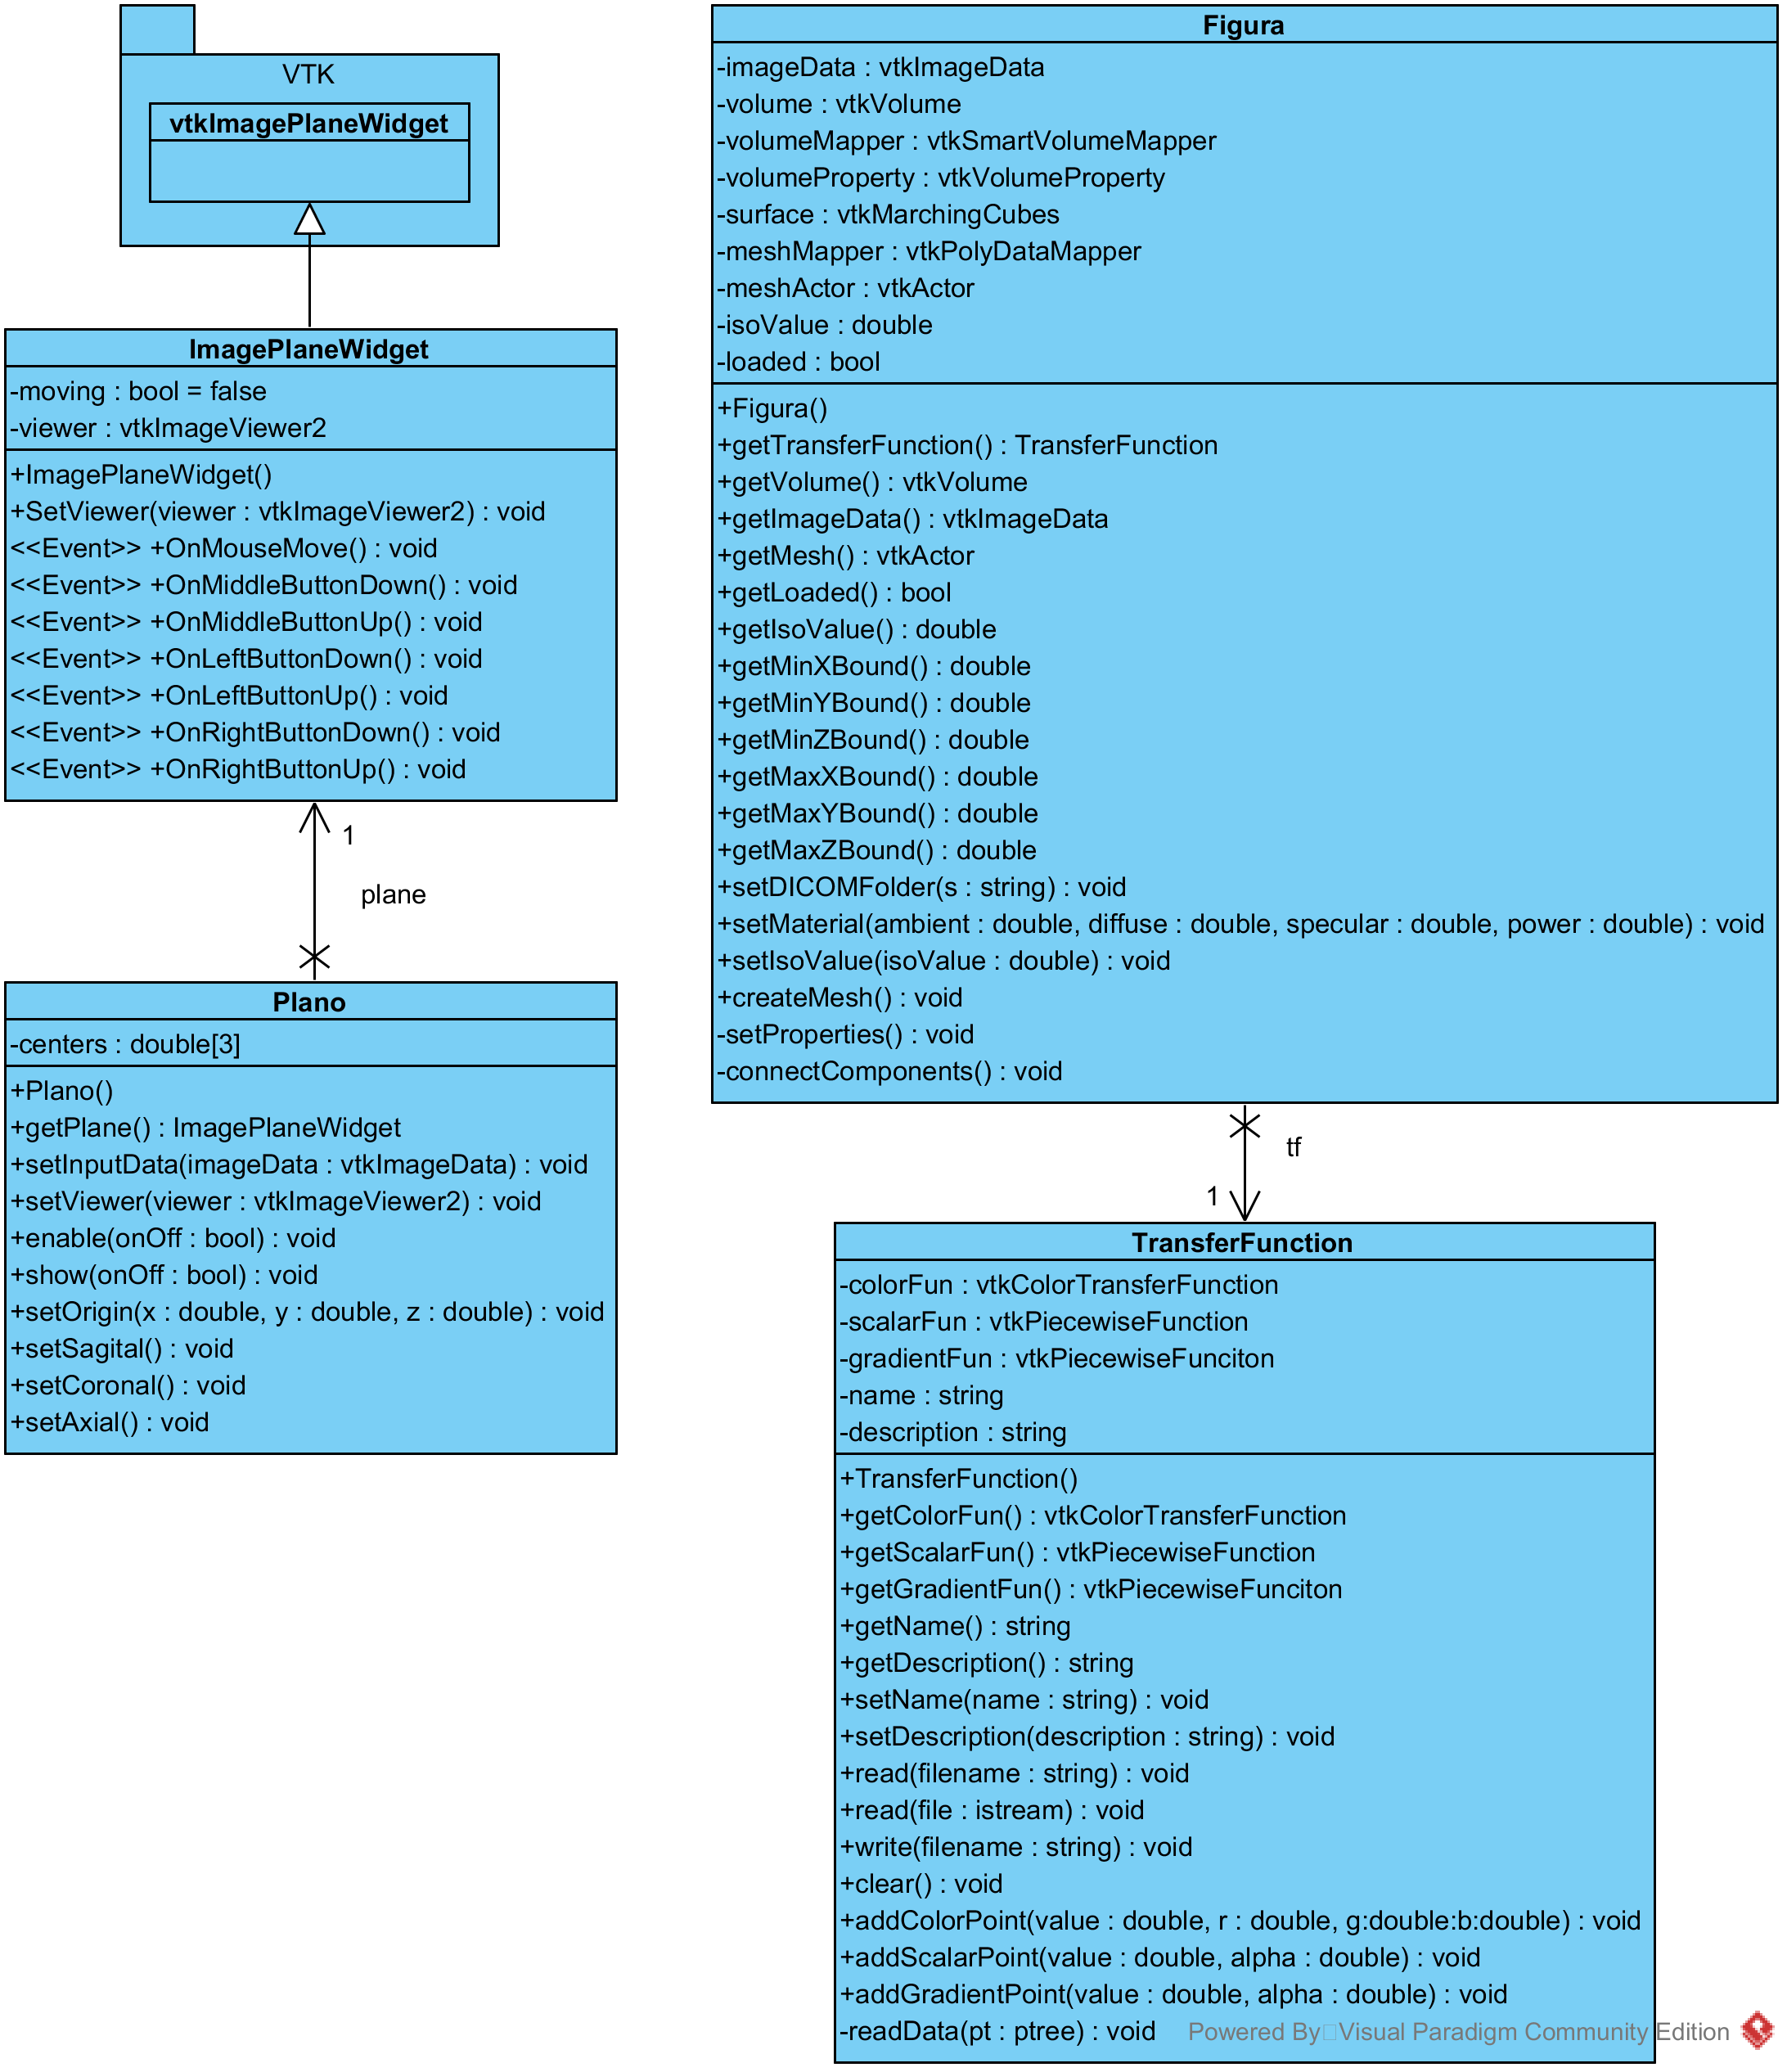
\includegraphics[width=12.5cm]{imagenes/diagramas/clases/Volume}
	\caption{Diagrama de clases del paquete \textit{Volume}}
	\label{fig:diagrama_clases_volume}
\end{figure}

\subsection{Charts}

\begin{figure}[H]
	\centering
	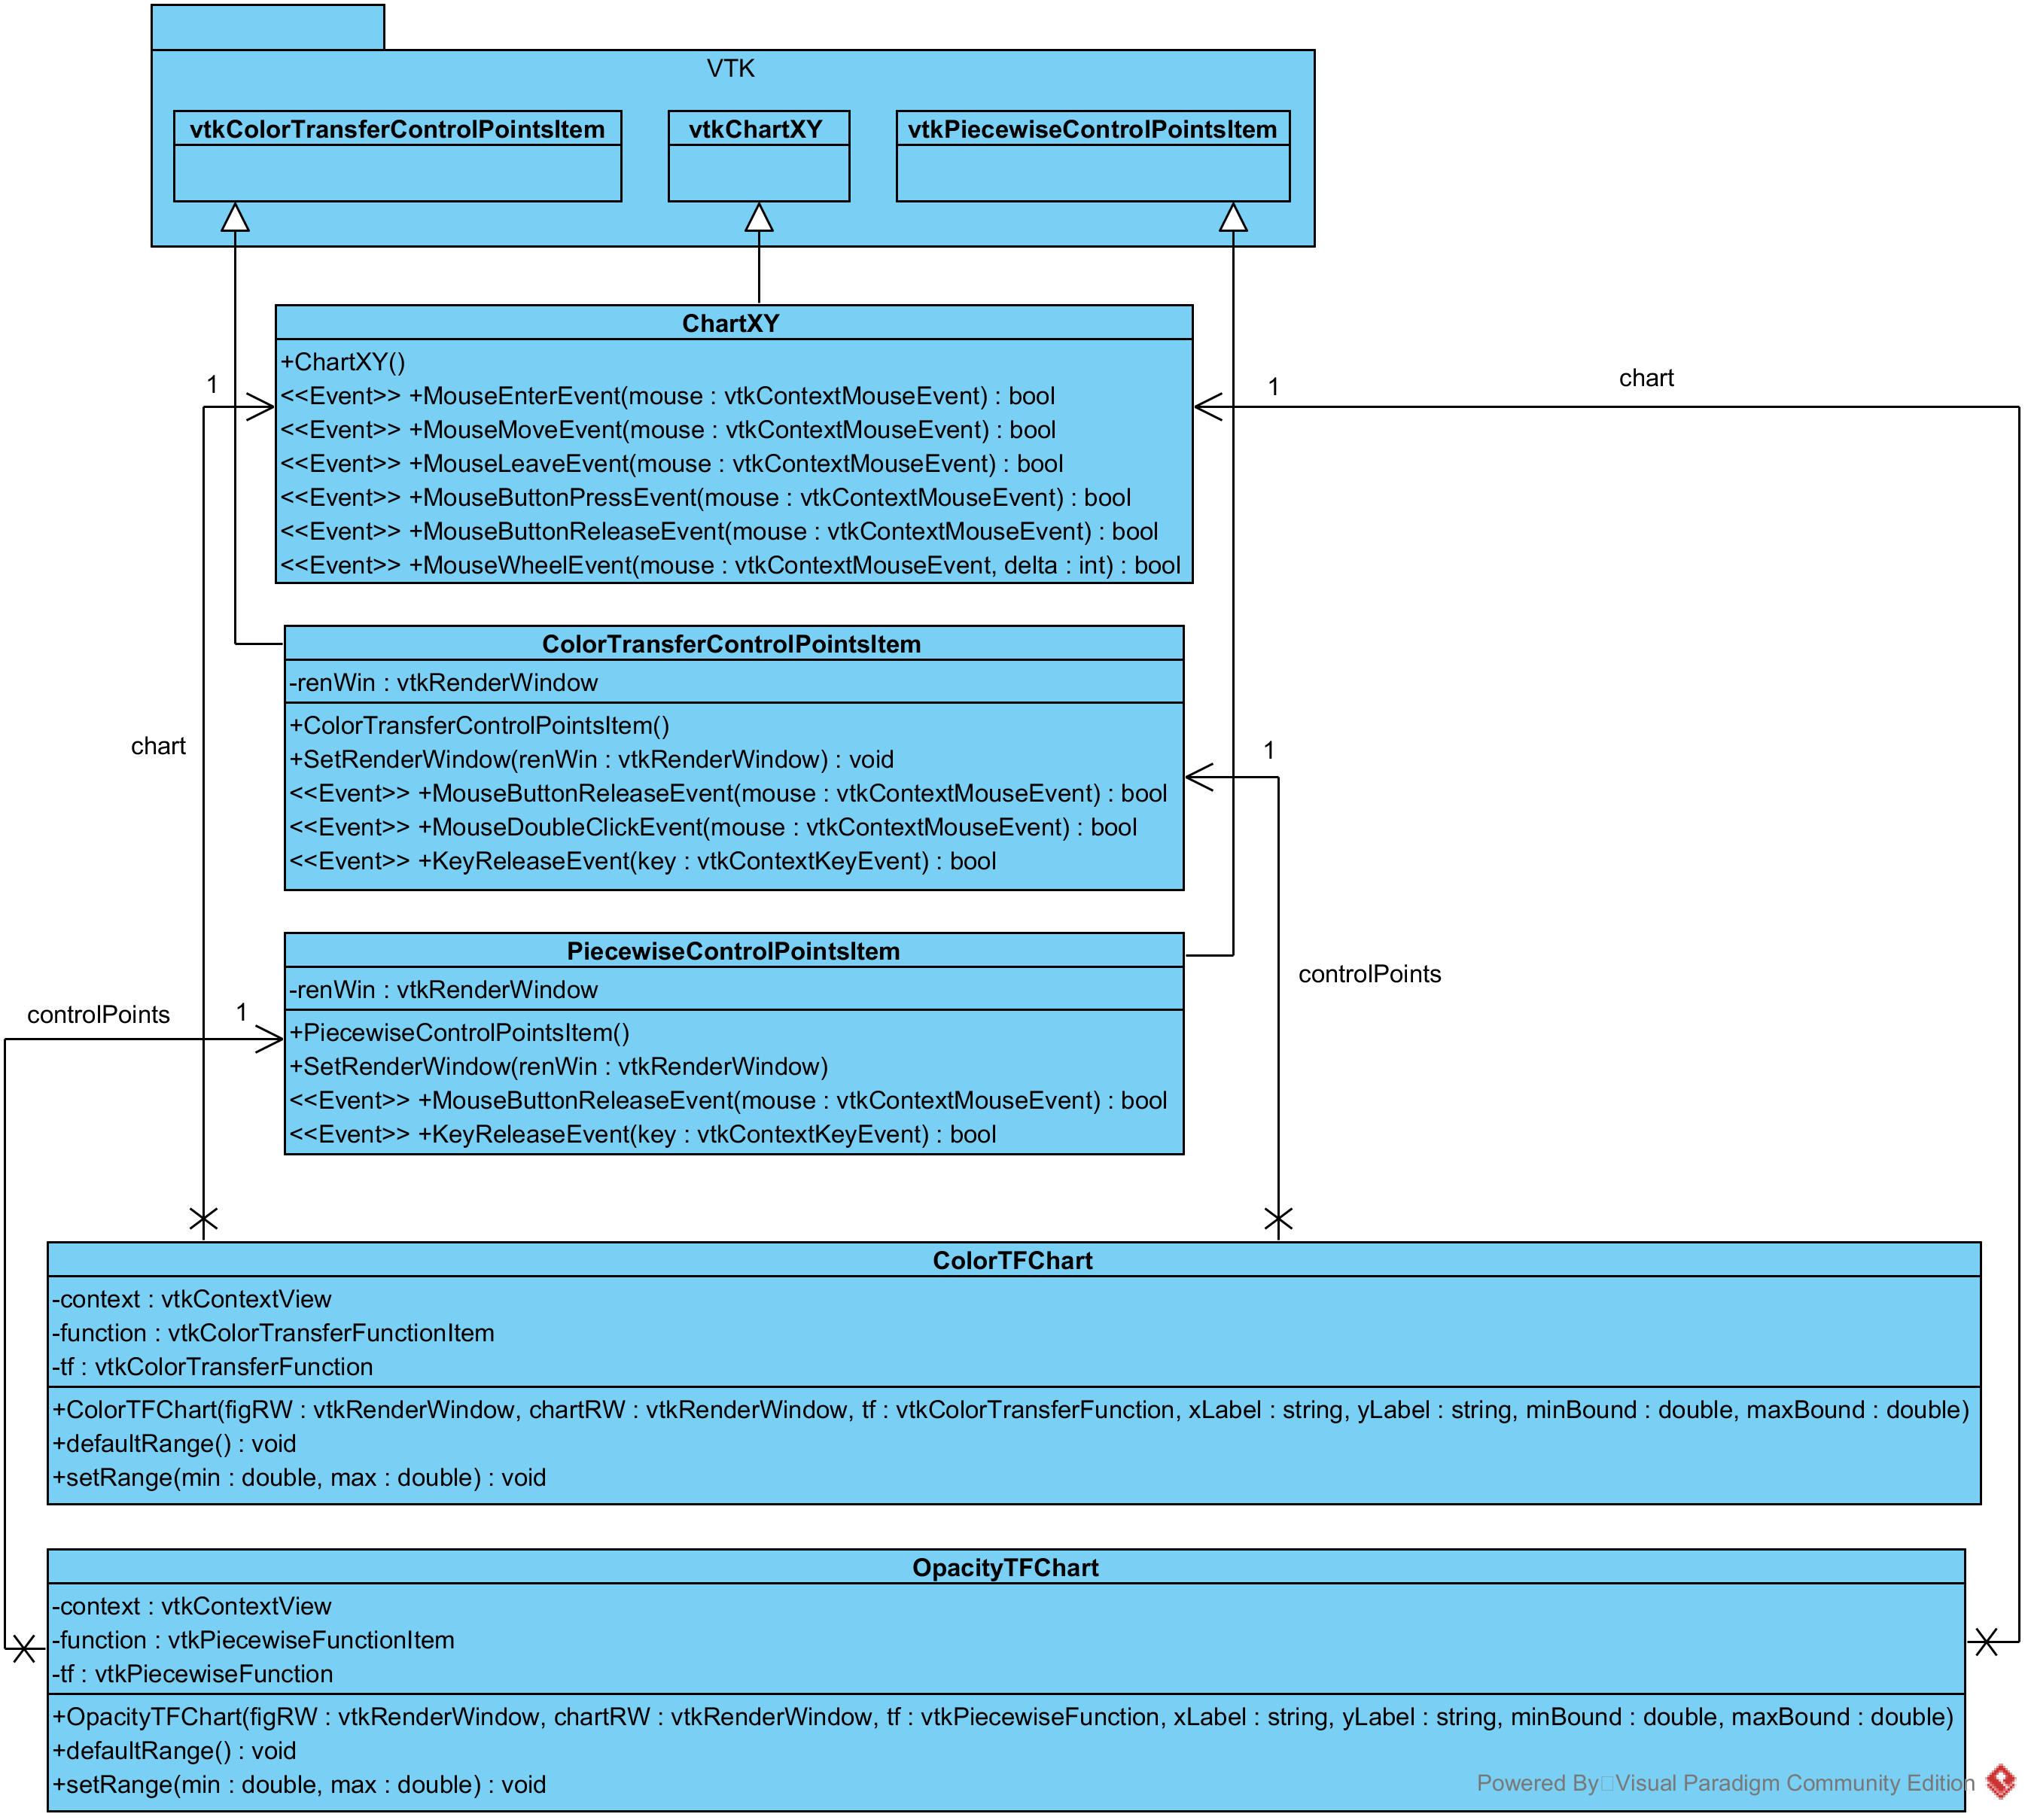
\includegraphics[width=12.5cm]{imagenes/diagramas/clases/Charts}
	\caption{Diagrama de clases del paquete \textit{Charts}}
	\label{fig:diagrama_clases_charts}
\end{figure}

\subsection{Application}

\begin{figure}[H]
	\centering
	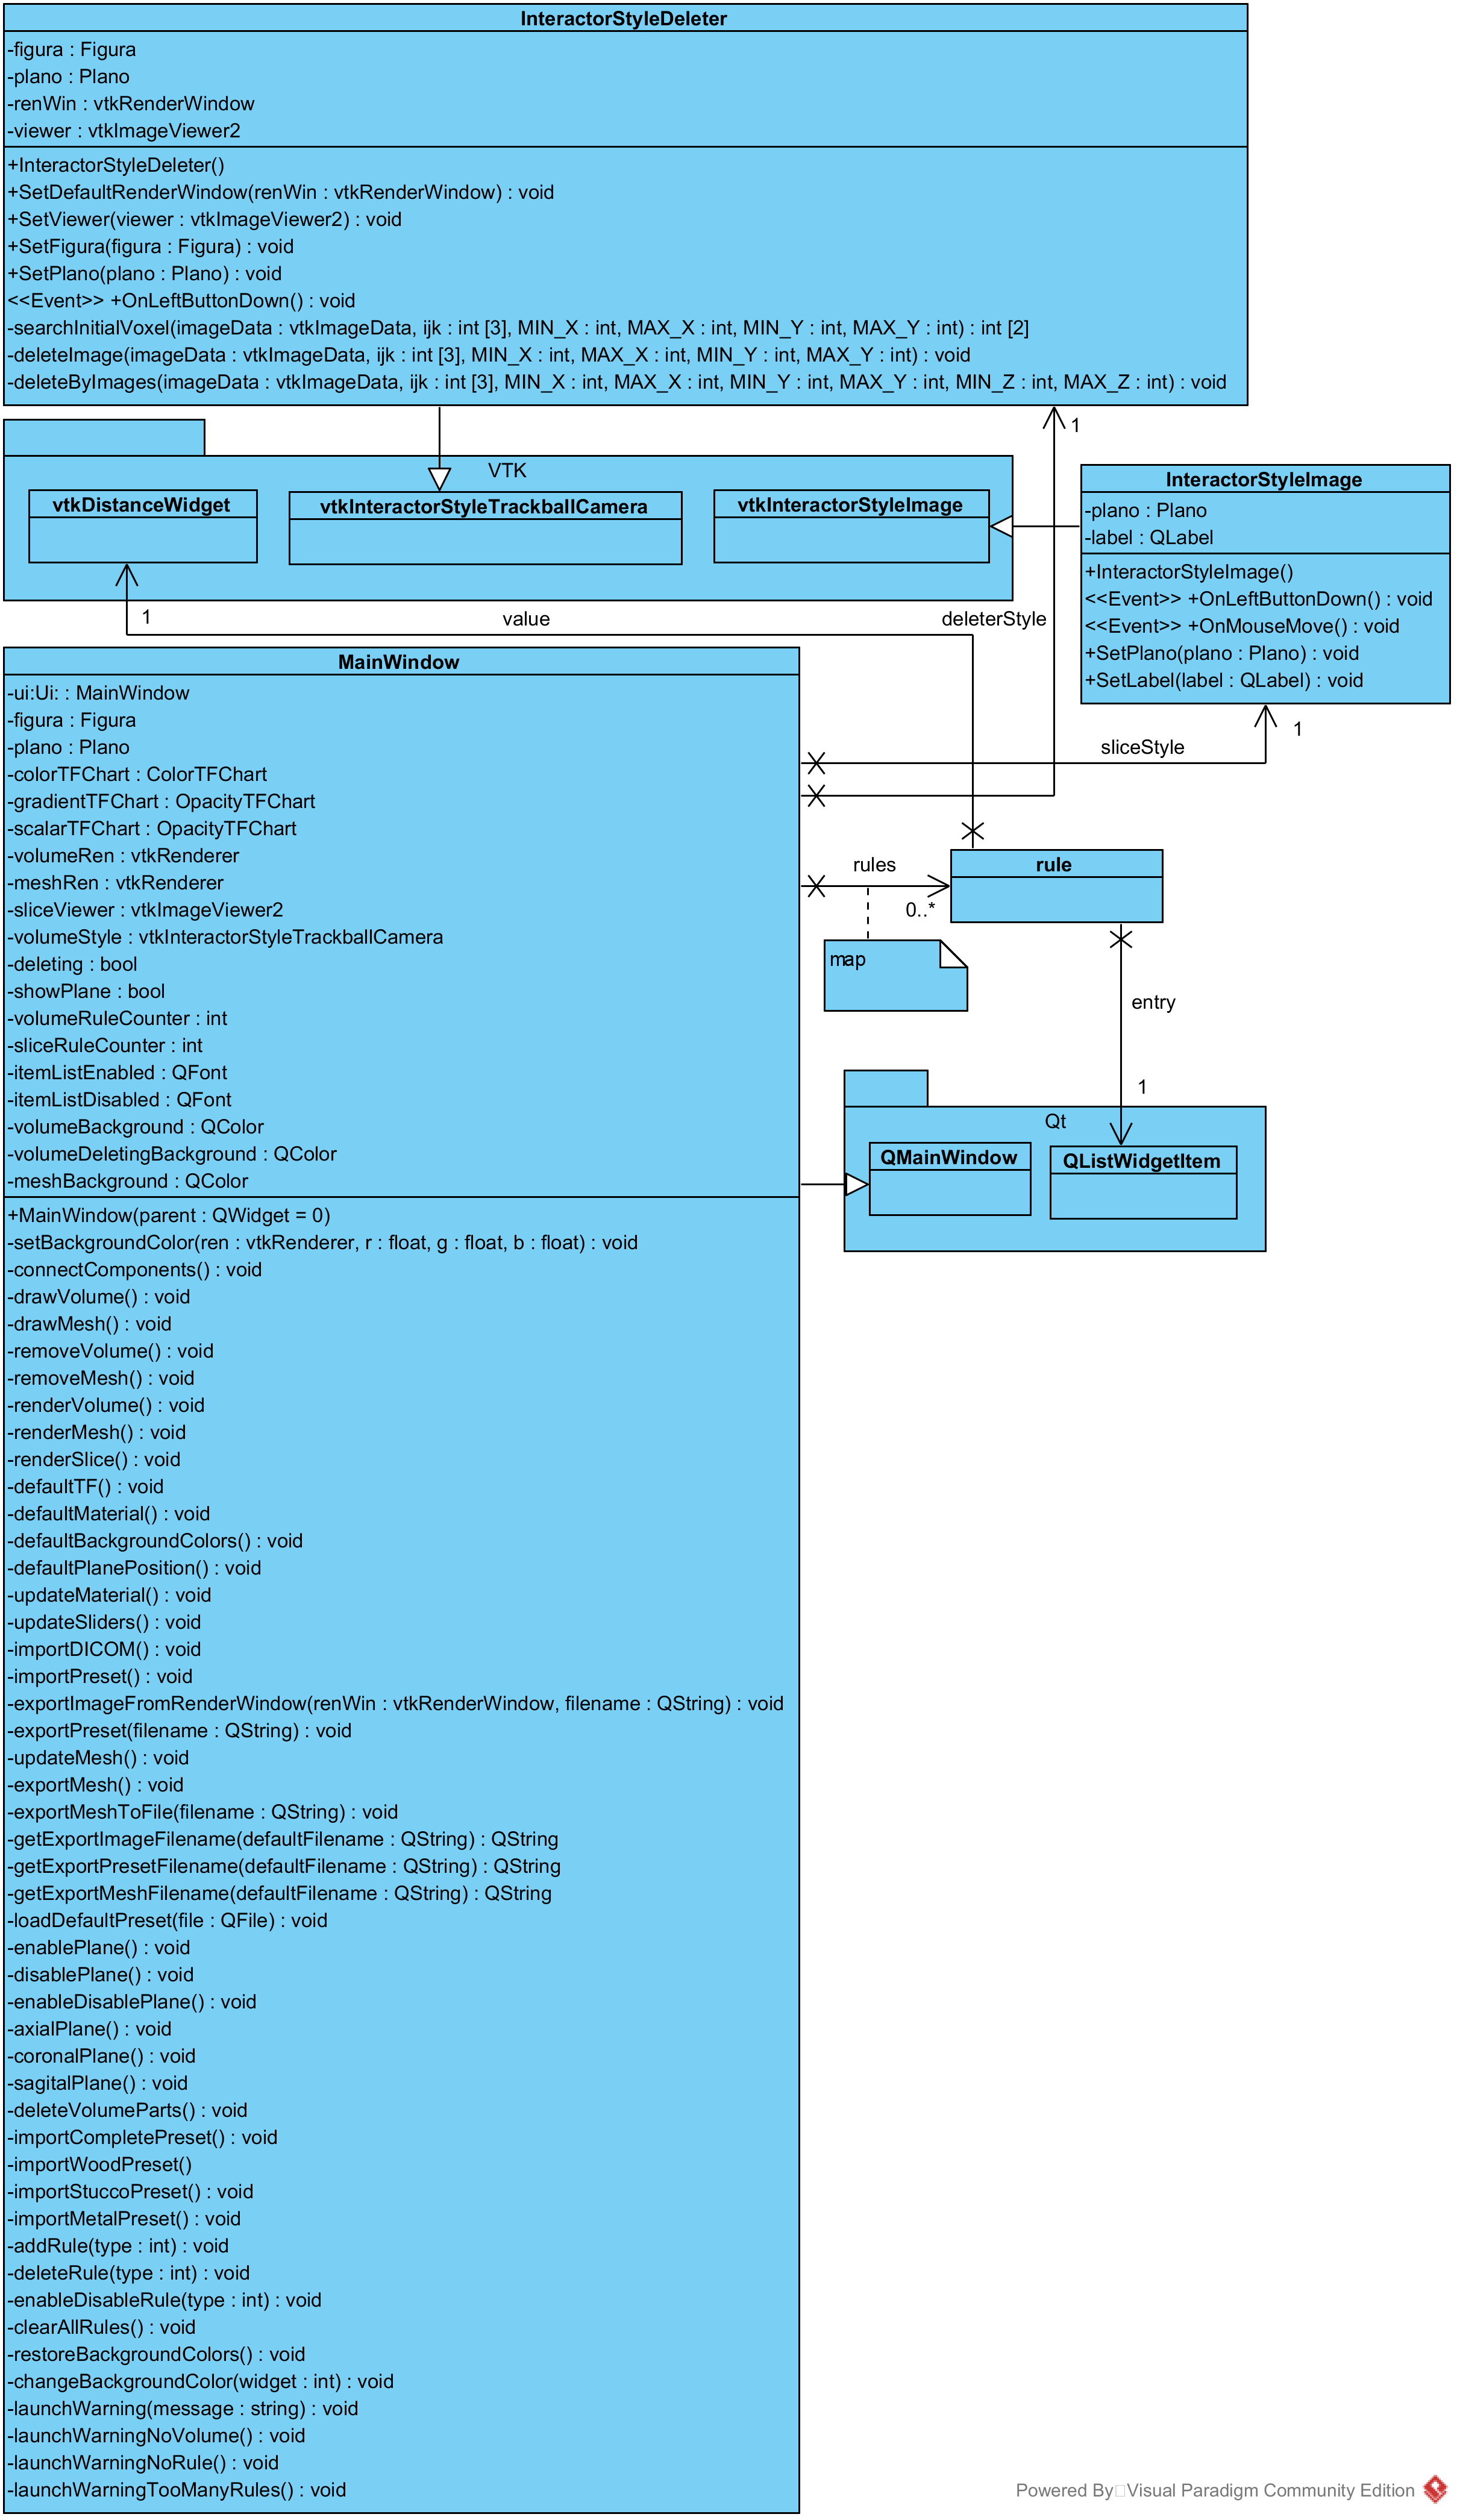
\includegraphics[width=10.5cm]{imagenes/diagramas/clases/Application}
	\caption{Diagrama de clases del paquete \textit{Application}}
	\label{fig:diagrama_clases_application}
\end{figure}

\section{Diagramas de secuencia}

A continuación se muestran algunos de los diagramas de secuencia de la aplicación: Aquellos que se han considerado más importantes.

\subsection{OpacityTFChart}

\begin{figure}[H]
	\centering
	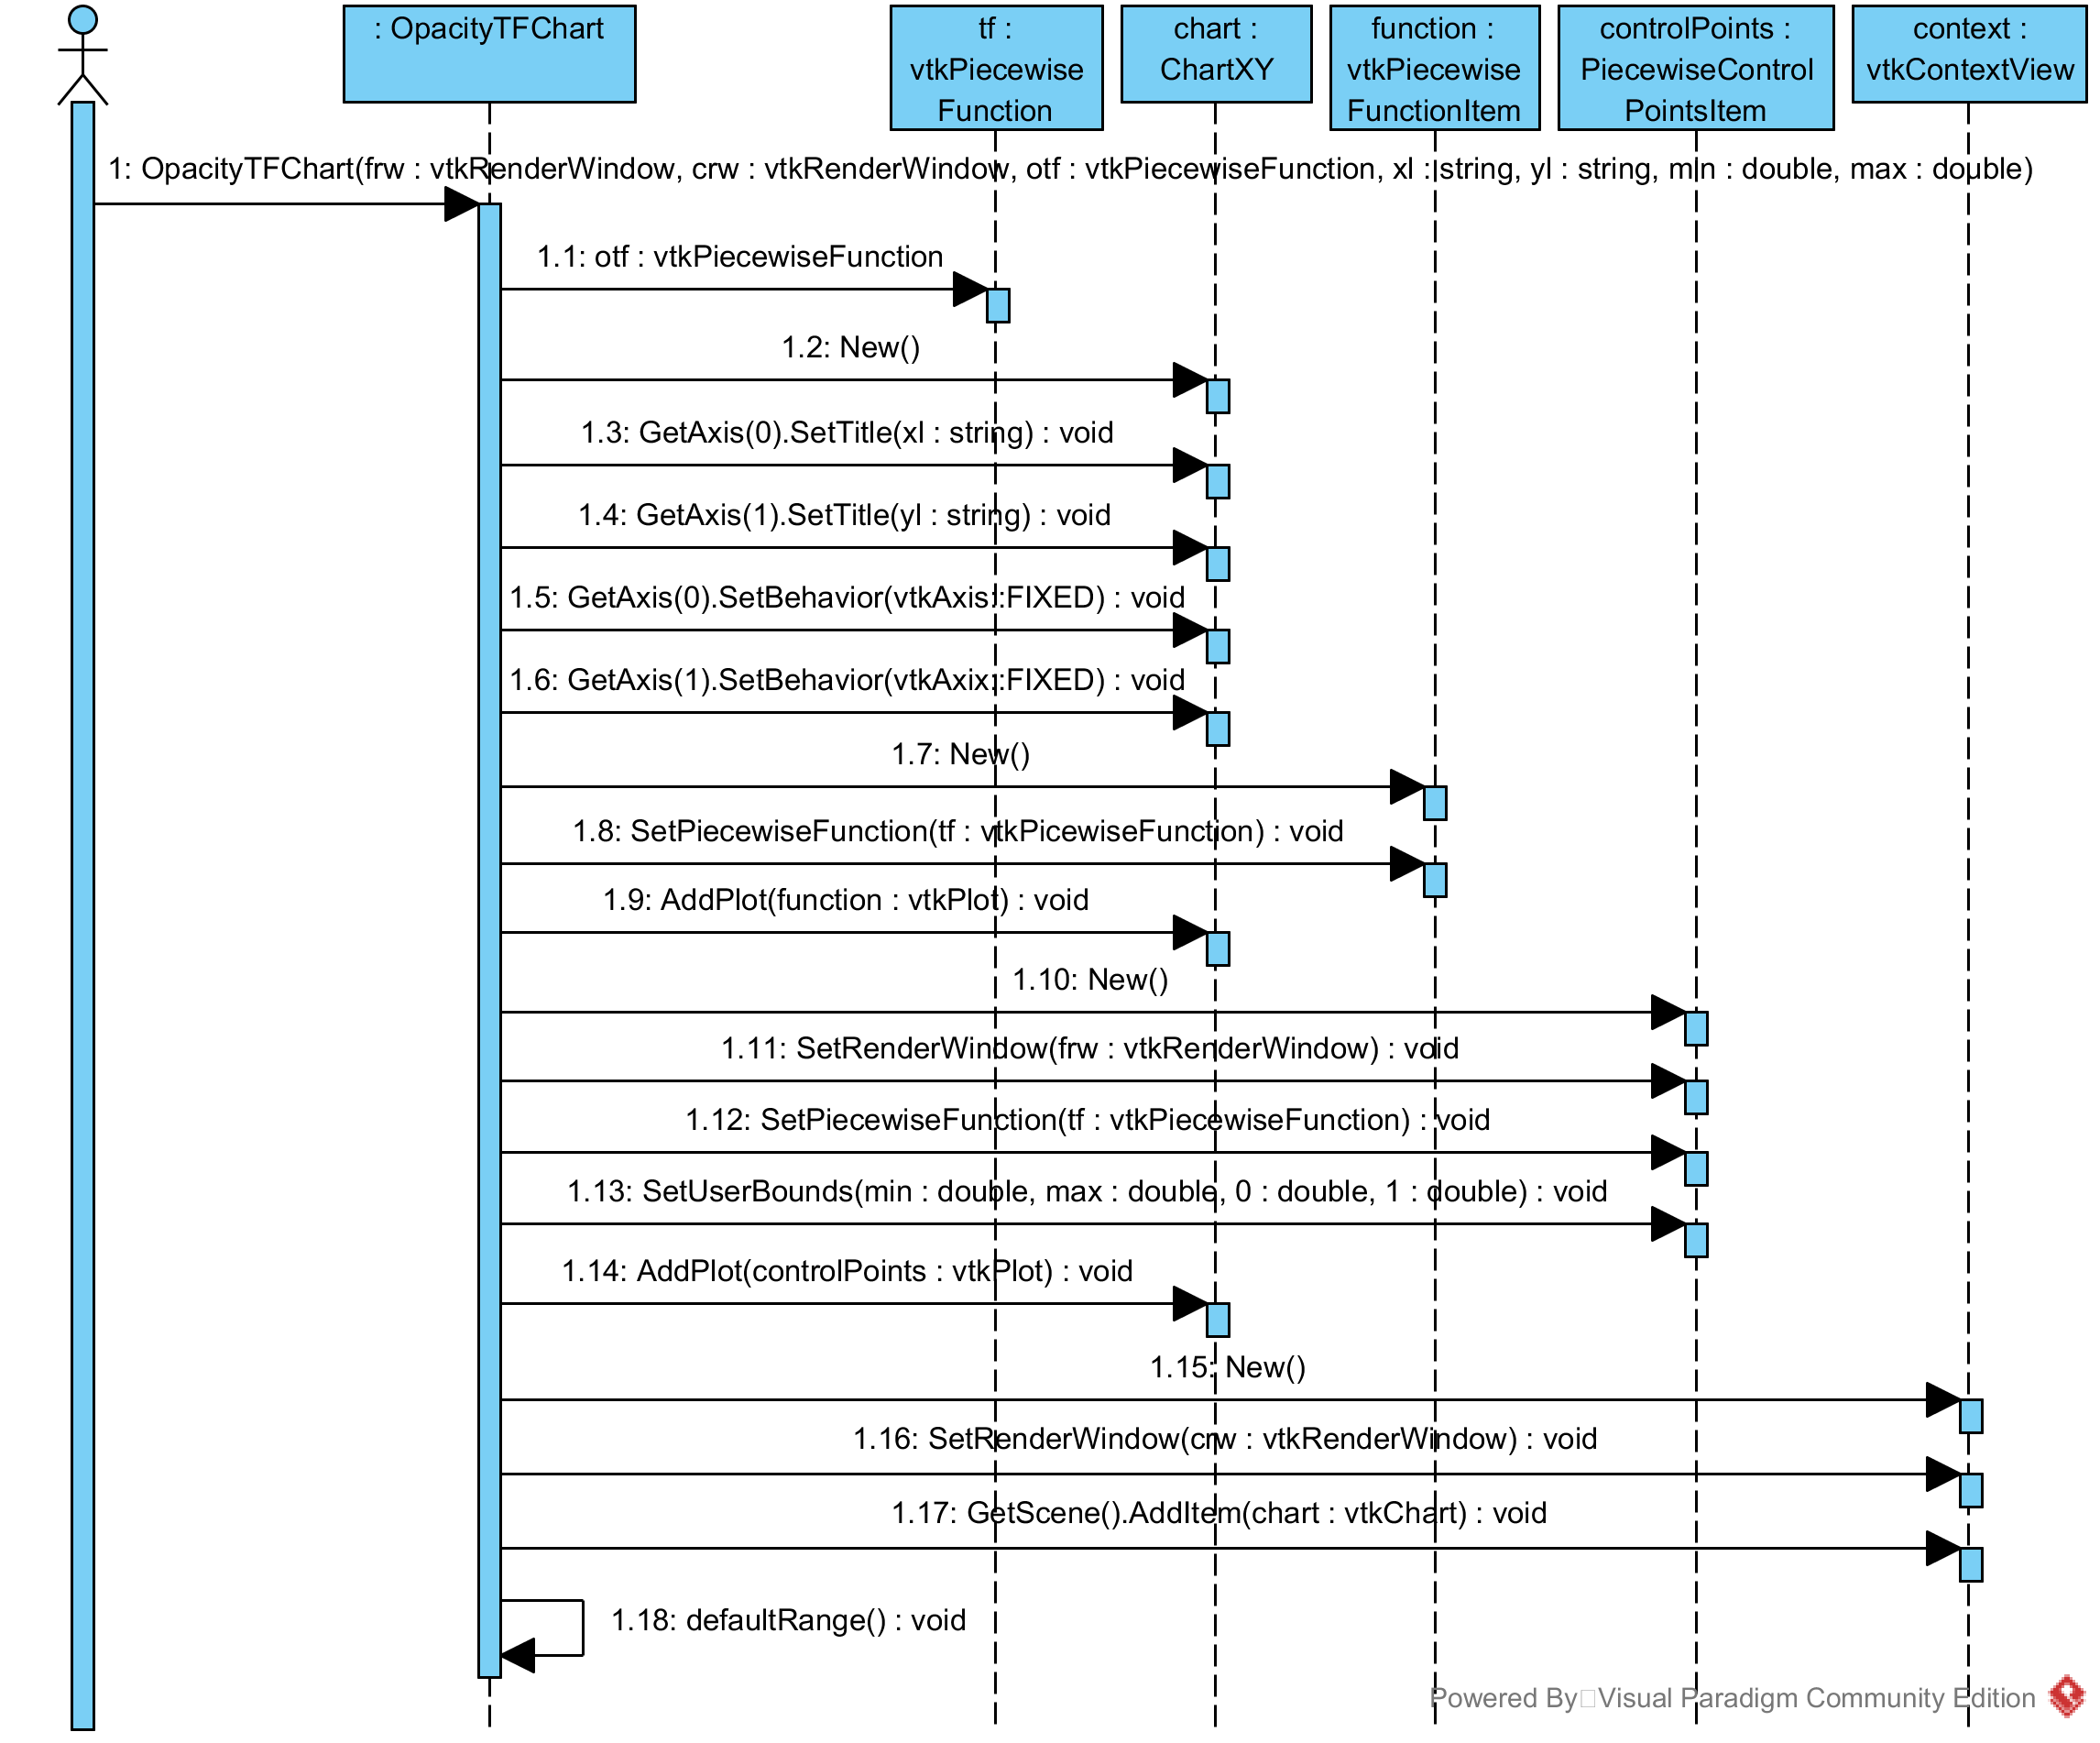
\includegraphics[angle=90,width=12cm]{imagenes/diagramas/secuencia/OpacityTFChart_New}
	\caption{Diagrama de secuencia del constructor de \textit{OpacityTFChart}}
	\label{fig:diagrama_secuencia_opacitytfchart_new}
\end{figure}

\subsection{ColorTFChart}

\begin{figure}[H]
	\centering
	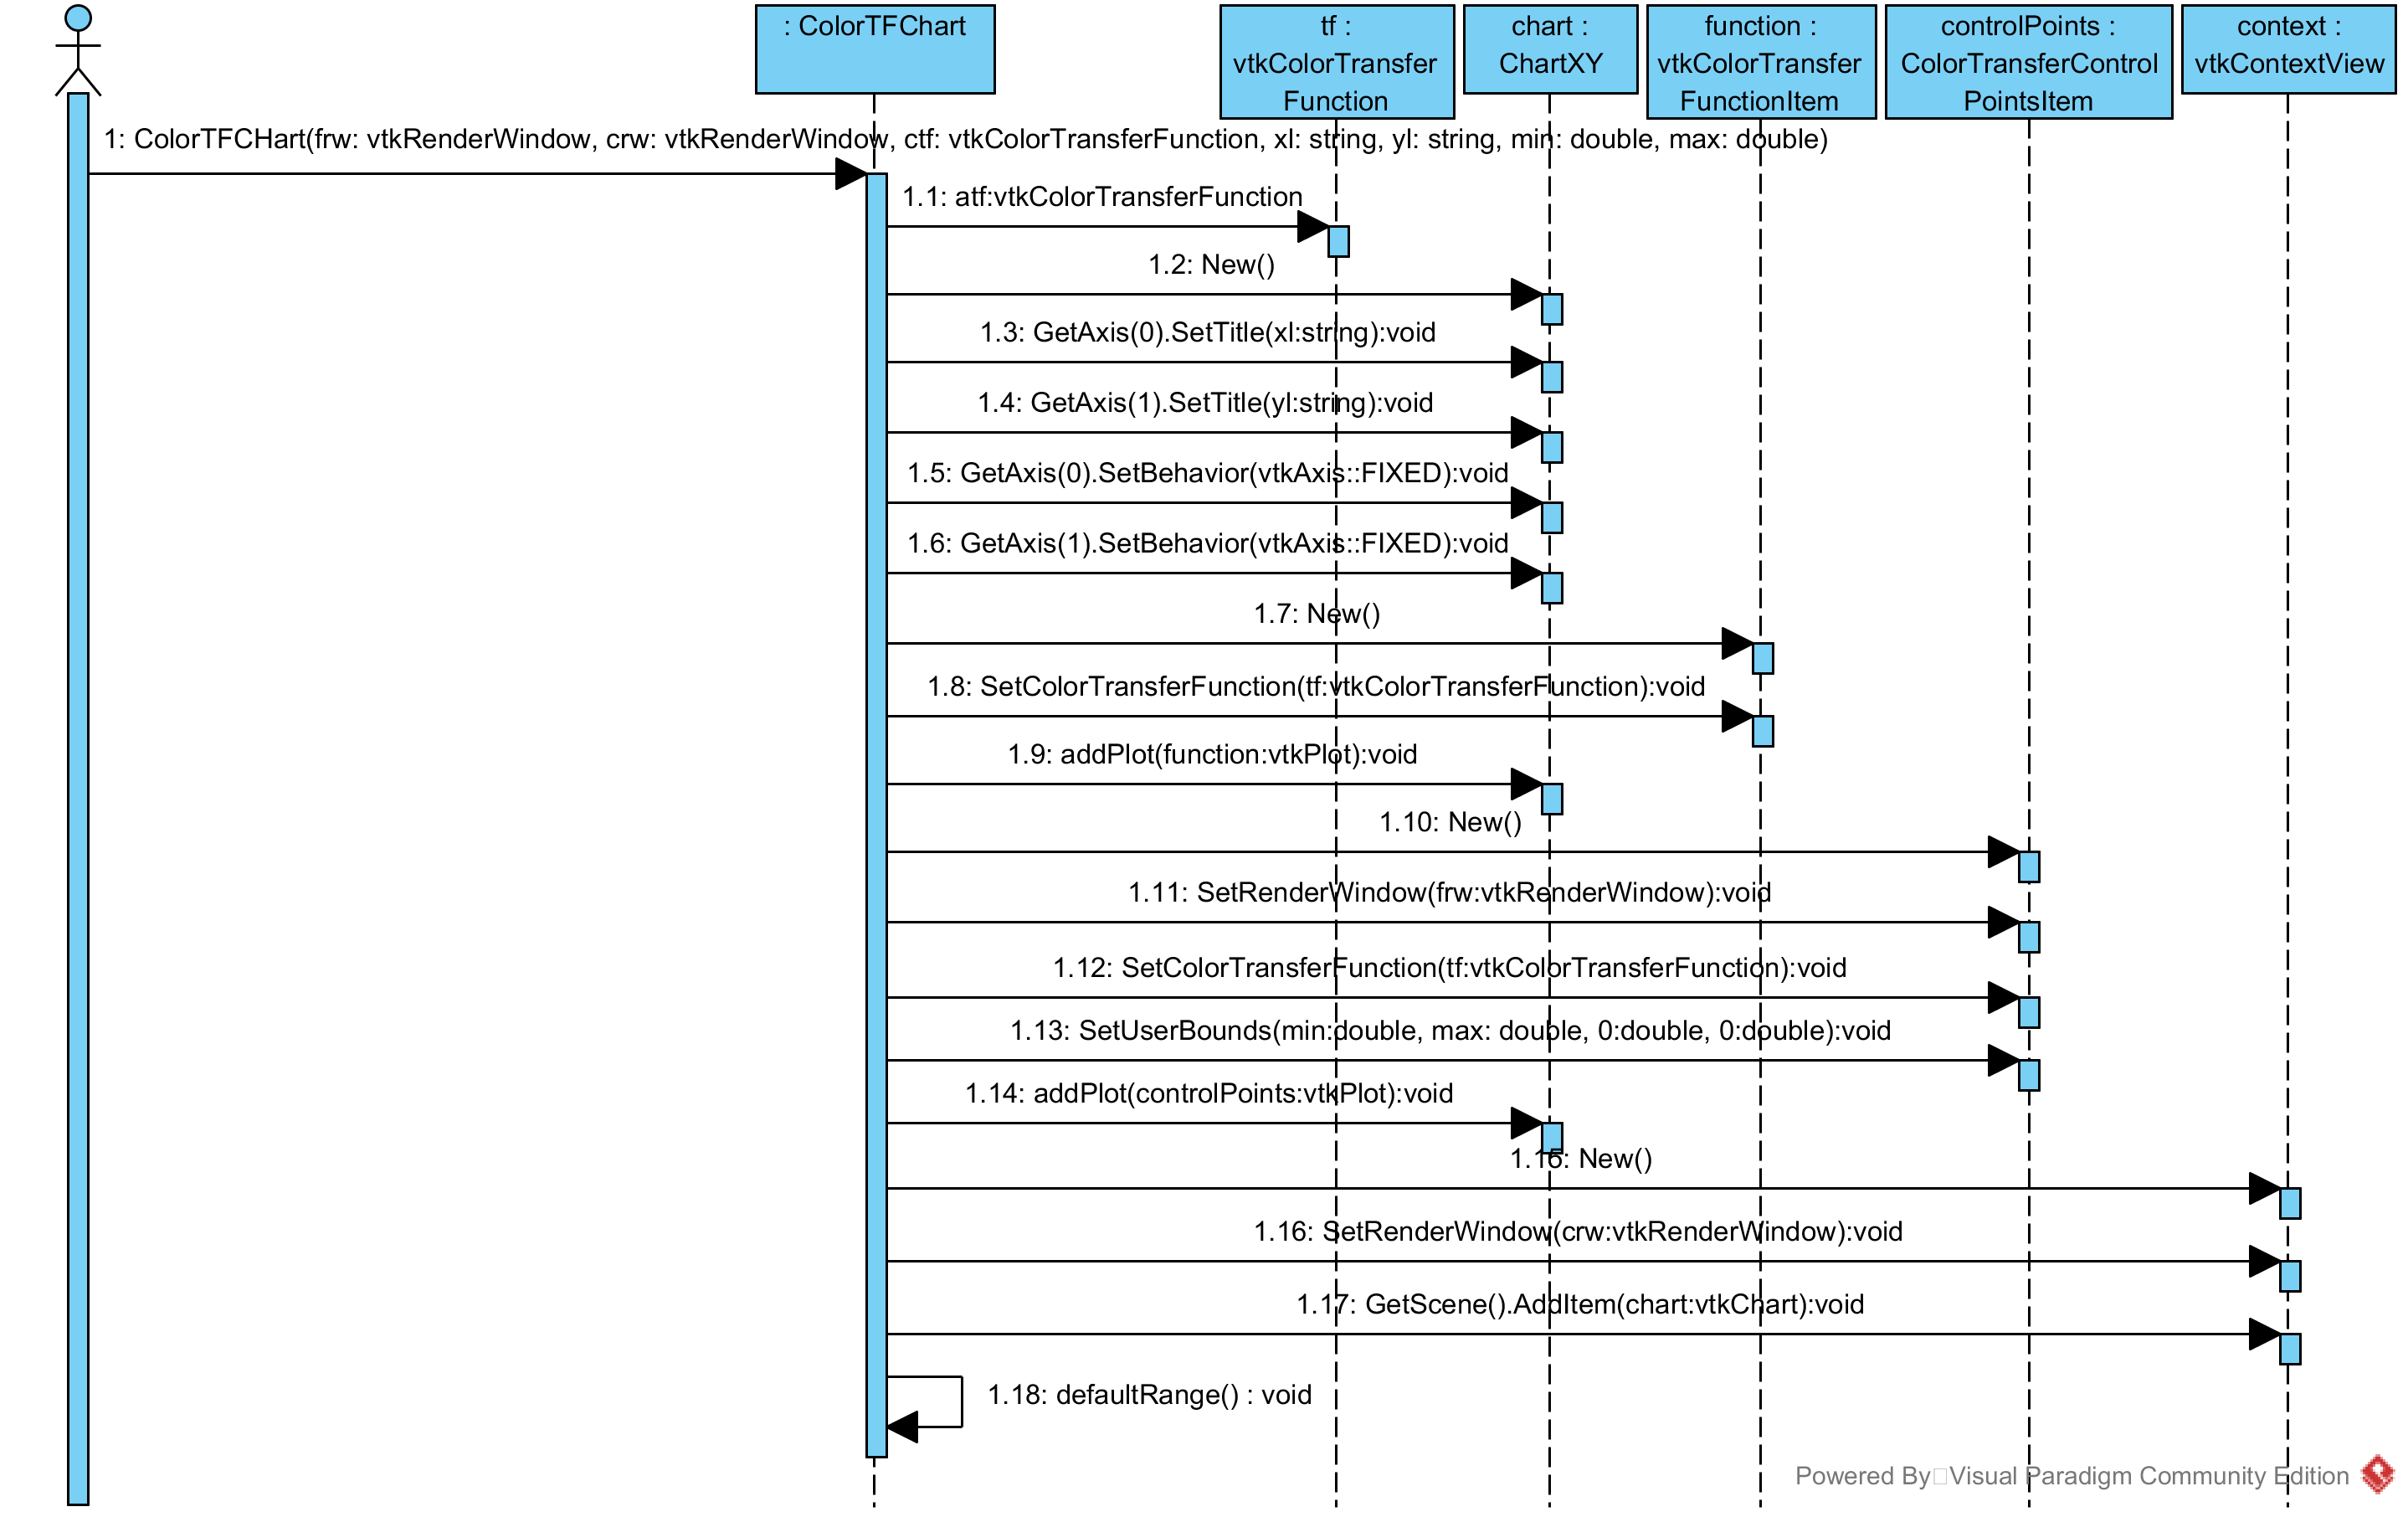
\includegraphics[angle=90,height=18cm]{imagenes/diagramas/secuencia/ColorTFChart_New}
	\caption{Diagrama de secuencia del constructor de \textit{ColorTFChart}}
	\label{fig:diagrama_secuencia_colortfchart_new}
\end{figure}

\subsection{ColorTransferControlPointsItem}

\begin{figure}[H]
	\centering
	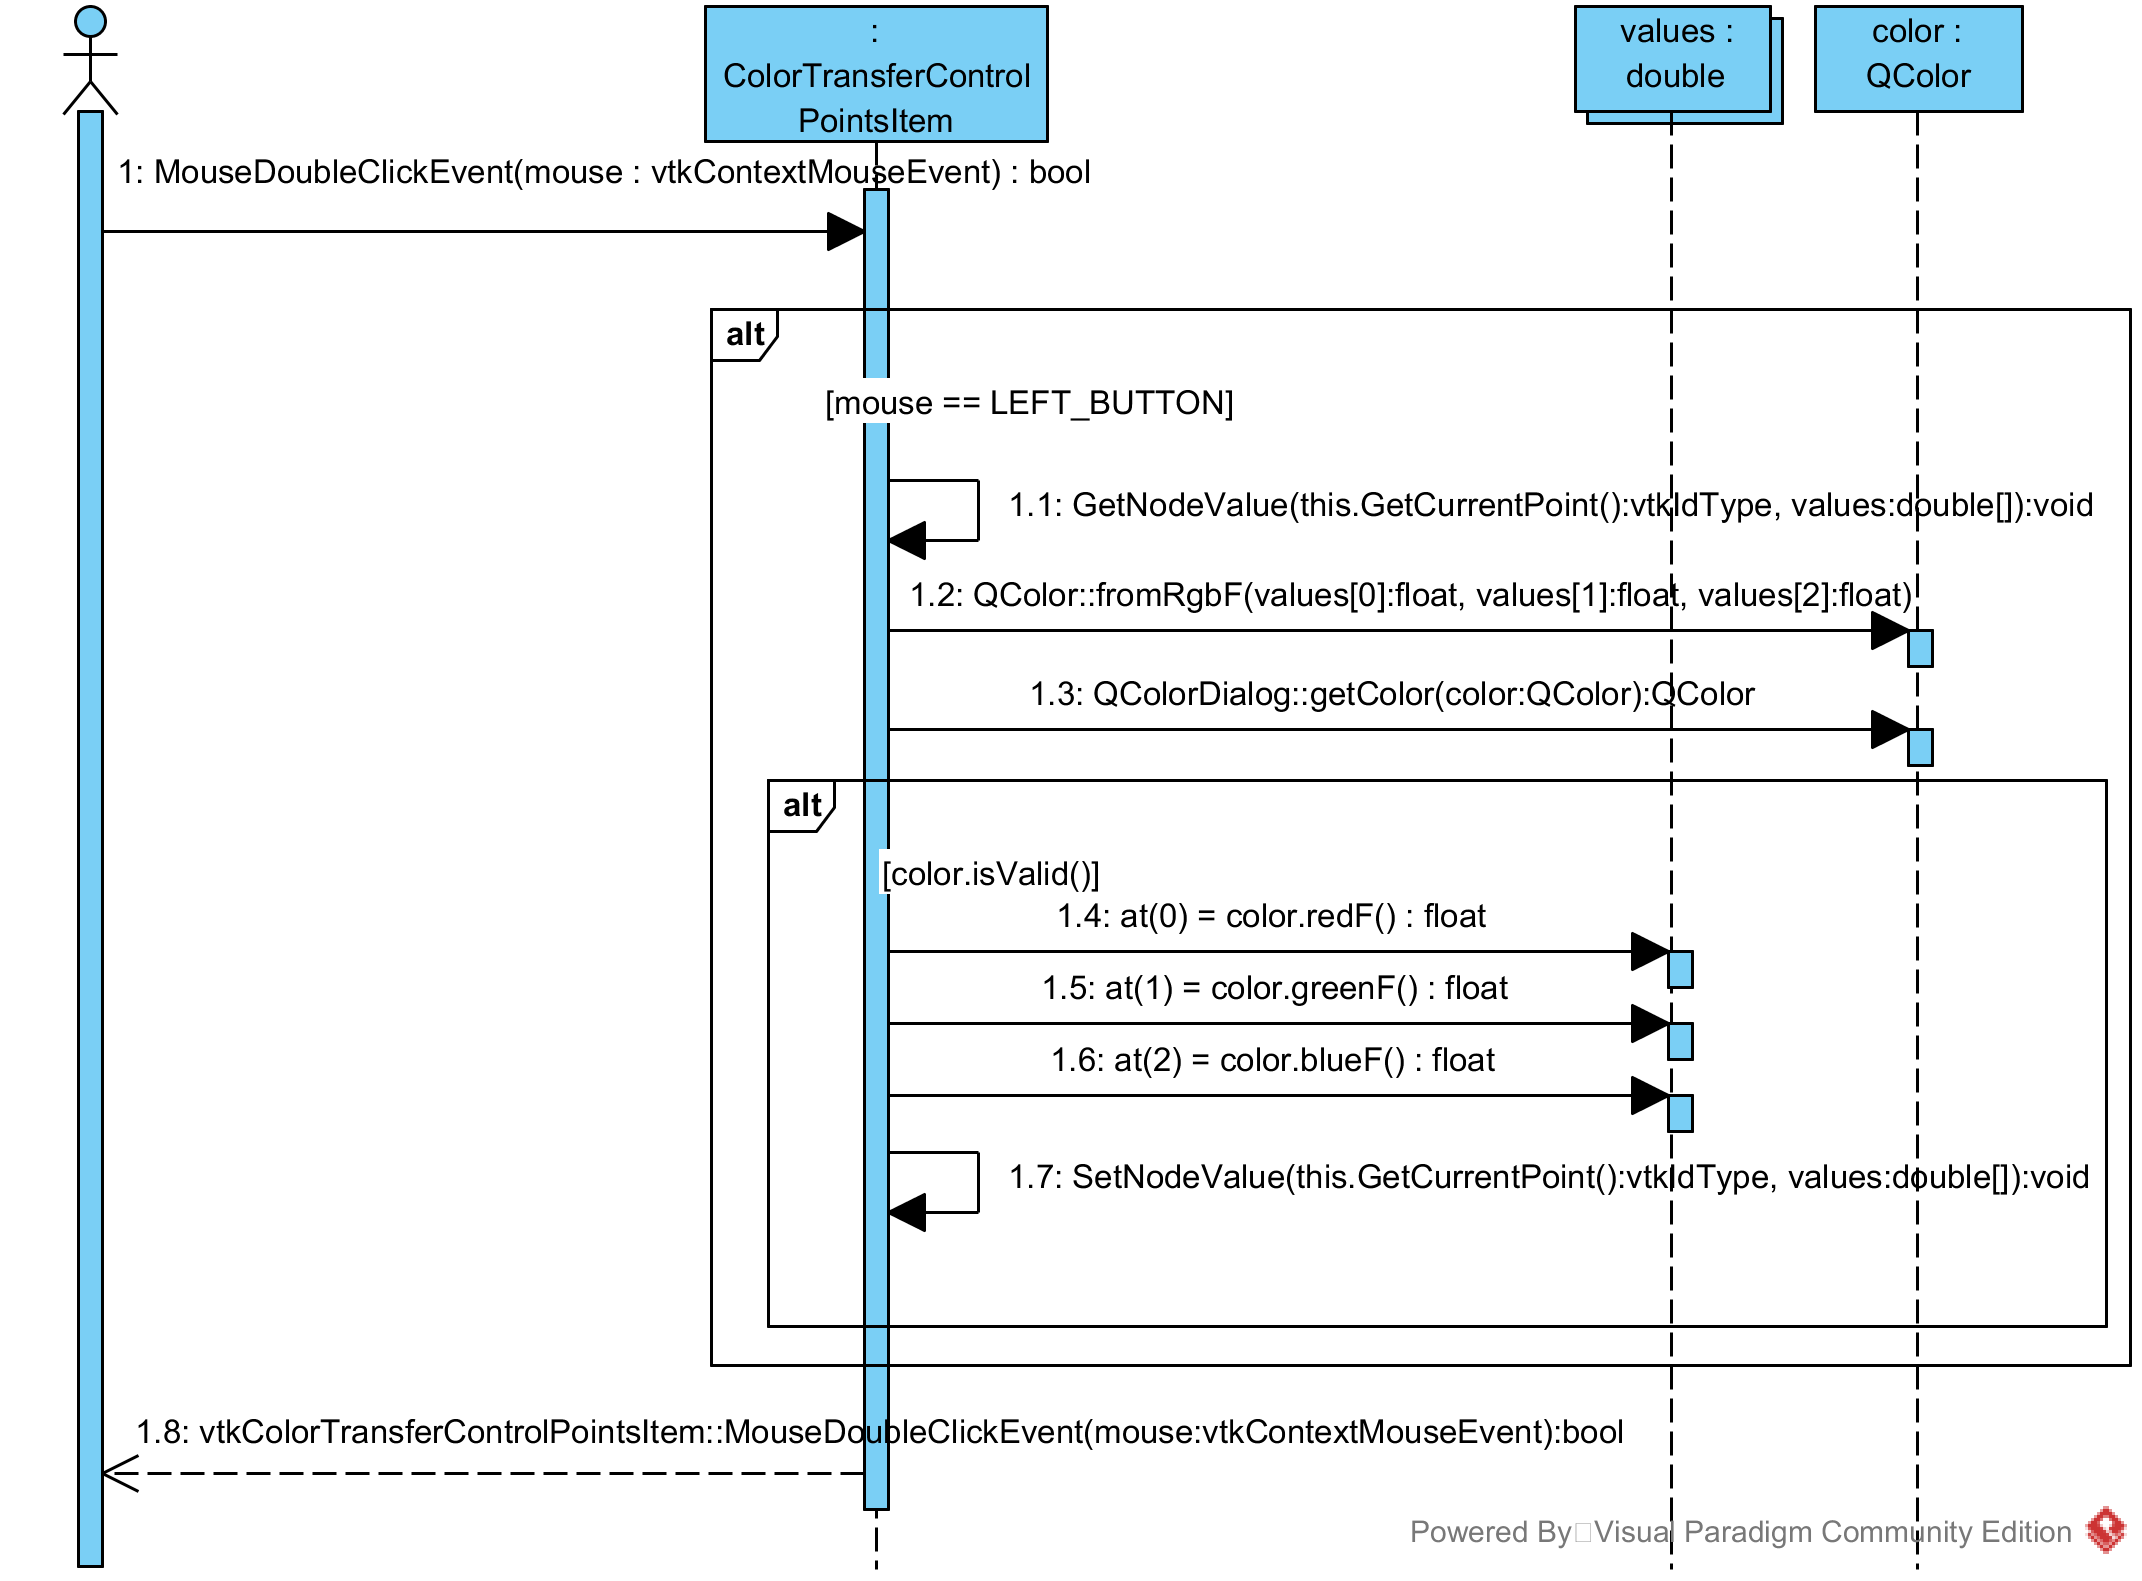
\includegraphics[angle=90,width=12cm]{imagenes/diagramas/secuencia/ColorTransferControlPointsItem_MouseDoubleClickEvent}
	\caption{Diagrama de secuencia del evento de doble click de \textit{ColorTransferControlPointsItem}}
	\label{fig:diagrama_secuencia_colortransfercontrolpointsitem_mousedoubleclickevent}
\end{figure}

\subsection{Figura}

\begin{figure}[H]
	\centering
	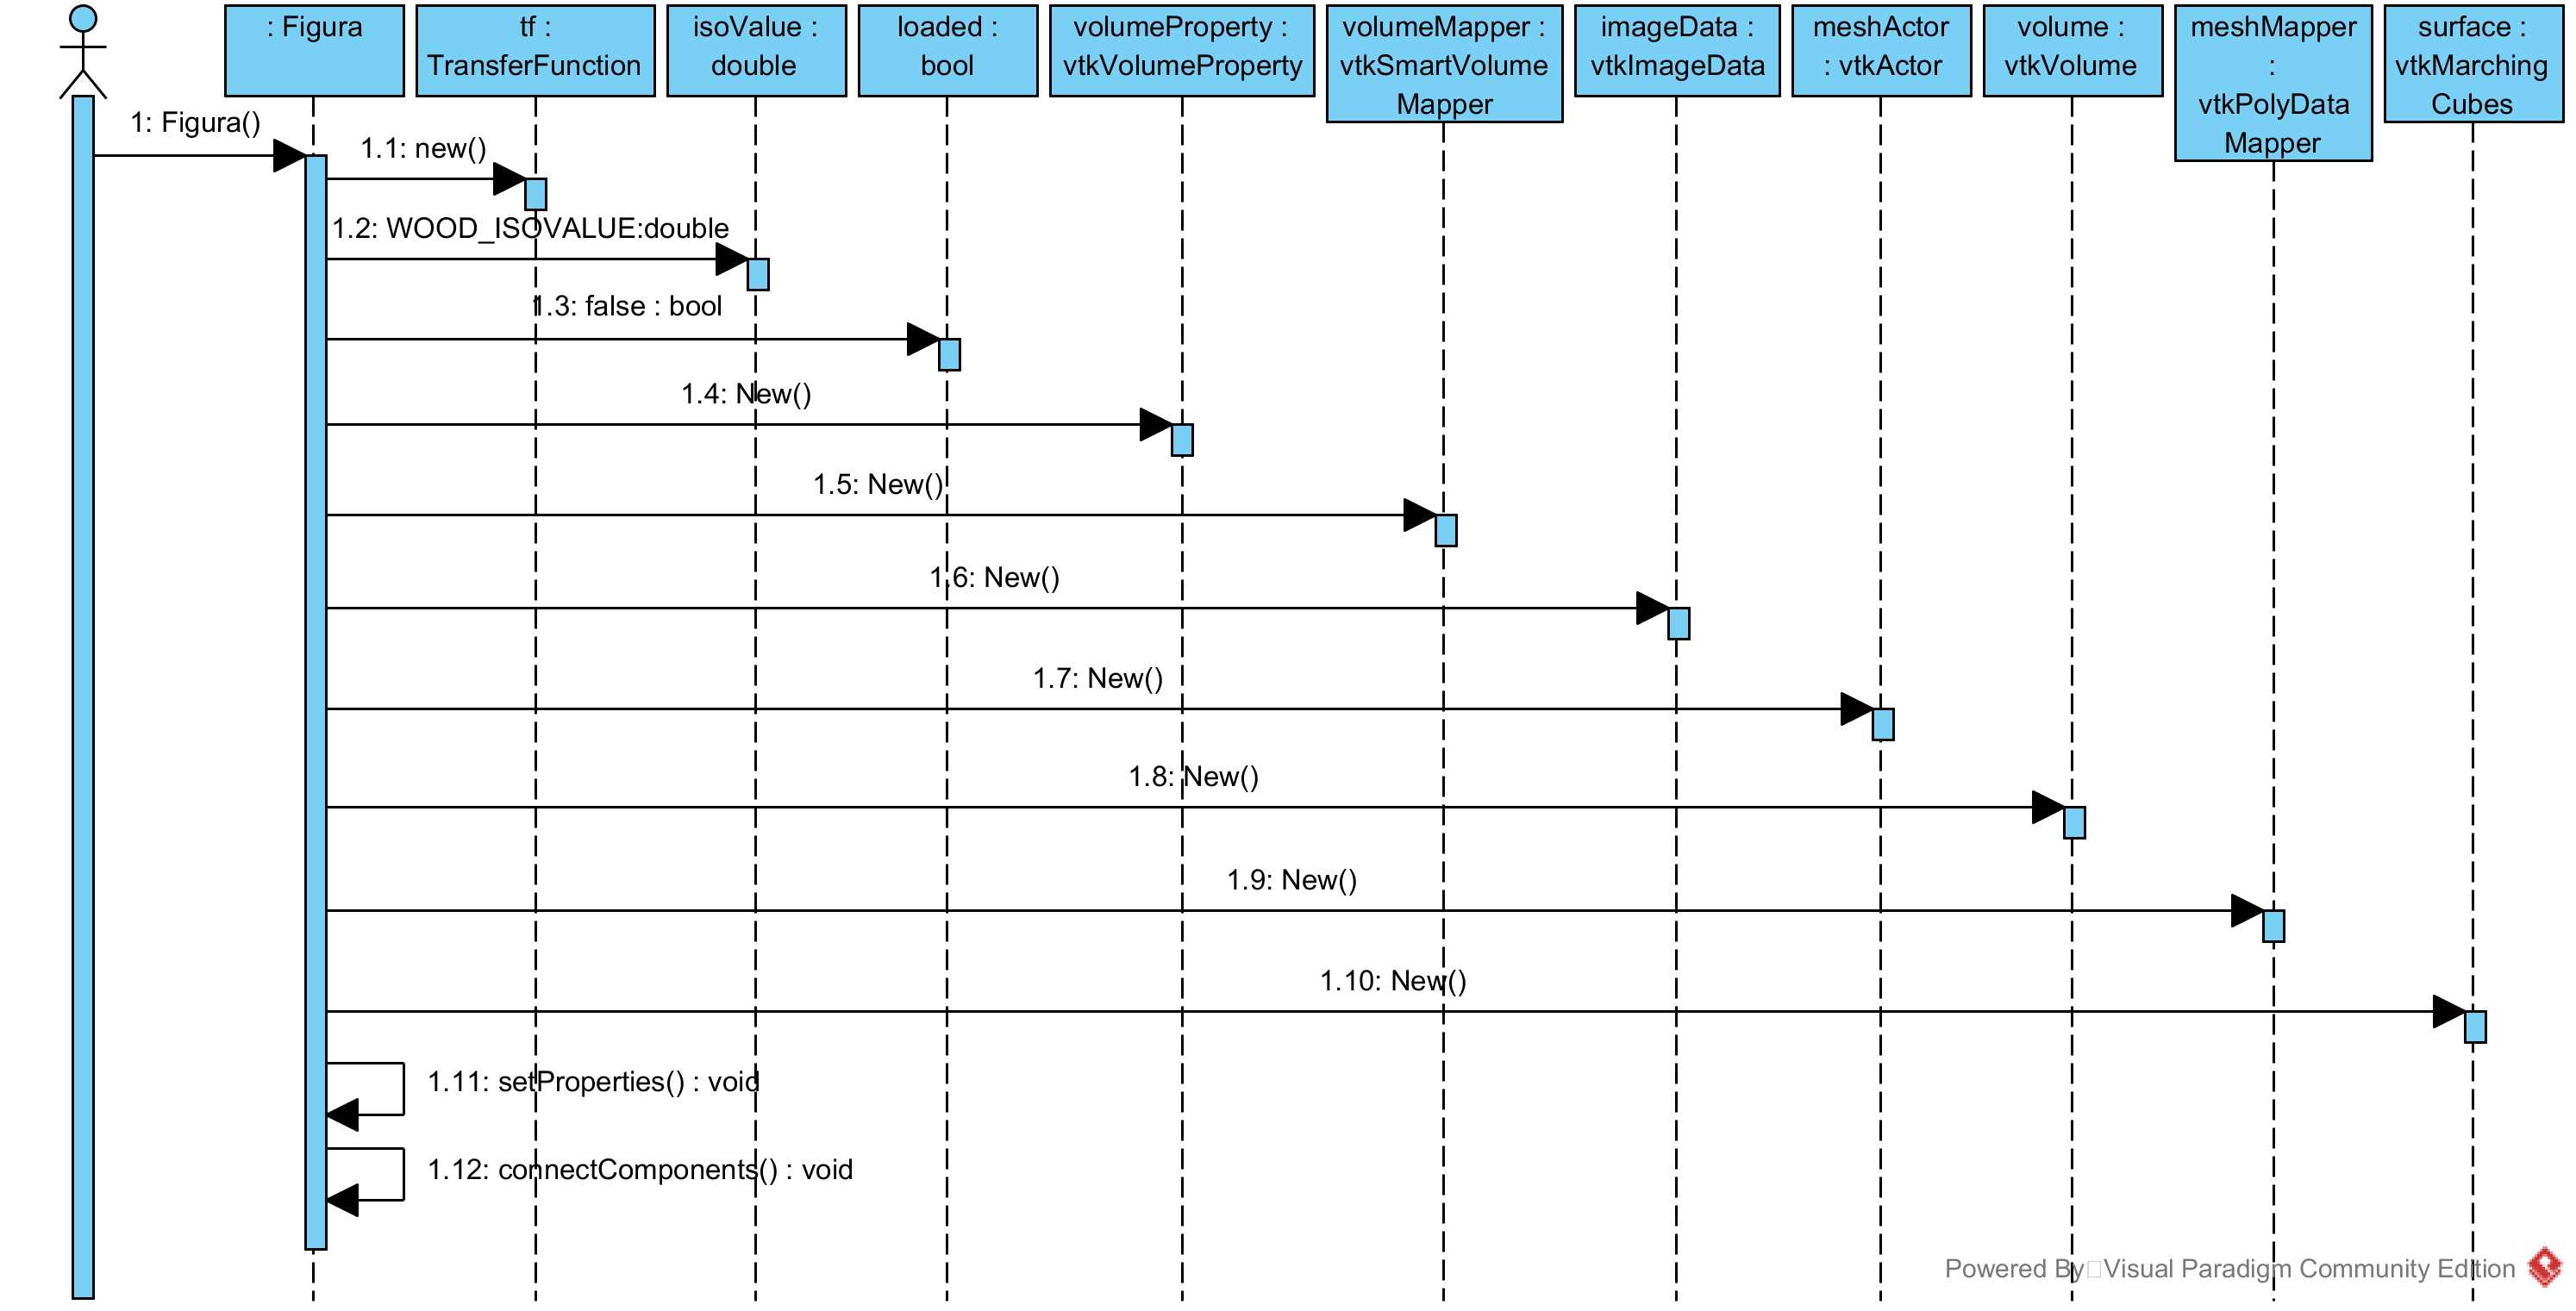
\includegraphics[angle=90,height=18cm]{imagenes/diagramas/secuencia/Figura_New}
	\caption{Diagrama de secuencia del constructor de \textit{Figura}}
	\label{fig:diagrama_secuencia_figura_new}
\end{figure}

\begin{figure}[H]
	\centering
	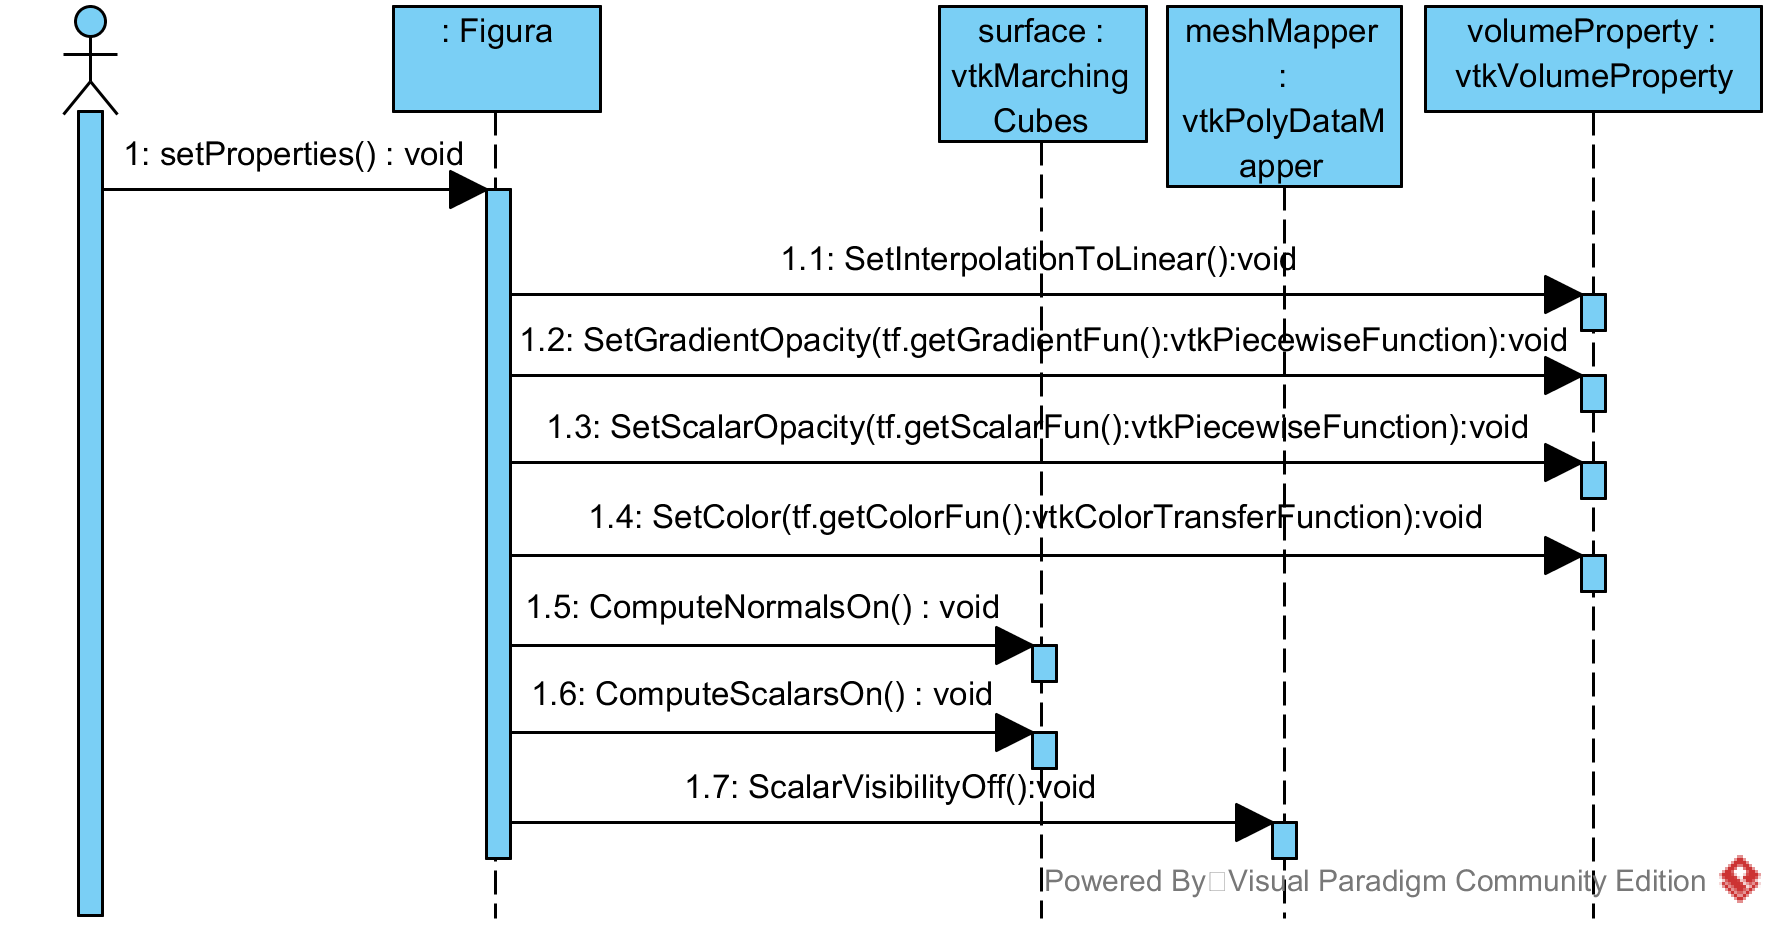
\includegraphics[width=12cm]{imagenes/diagramas/secuencia/Figura_SetProperties}
	\caption{Diagrama de secuencia del método \textit{setProperties} de \textit{Figura}}
	\label{fig:diagrama_secuencia_figura_setproperties}
\end{figure}

\begin{figure}[H]
	\centering
	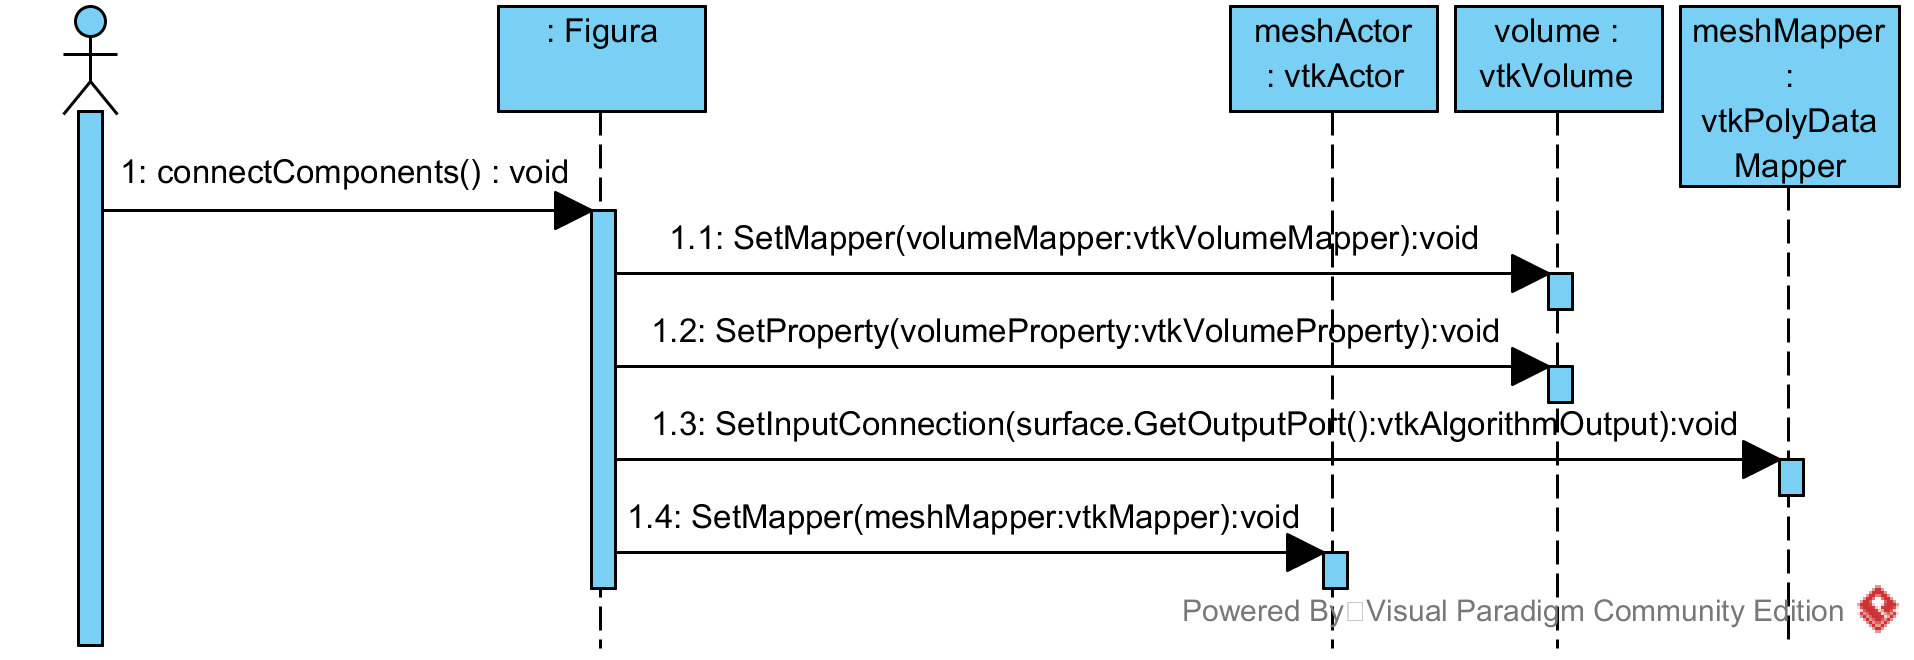
\includegraphics[width=12cm]{imagenes/diagramas/secuencia/Figura_ConnectComponents}
	\caption{Diagrama de secuencia del método \textit{connectComponents} de \textit{Figura}}
	\label{fig:diagrama_secuencia_figura_connectcomponents}
\end{figure}

\begin{figure}[H]
	\centering
	\includegraphics[angle=90,height=18cm]{imagenes/diagramas/secuencia/Figura_SetDicomFolder}
	\caption{Diagrama de secuencia del método \textit{setDICOMFolder} de \textit{Figura}}
	\label{fig:diagrama_secuencia_figura_setdicomfolder}
\end{figure}

\subsection{TransferFunction}

\begin{figure}[H]
	\centering
	\includegraphics[width=10cm]{imagenes/diagramas/secuencia/TransferFunction_ReadFromString}
	\caption{Diagrama de secuencia del método \textit{read} de \textit{TransferFunction}}
	\label{fig:diagrama_secuencia_transferfunction_read}
\end{figure}

\begin{figure}[H]
	\centering
	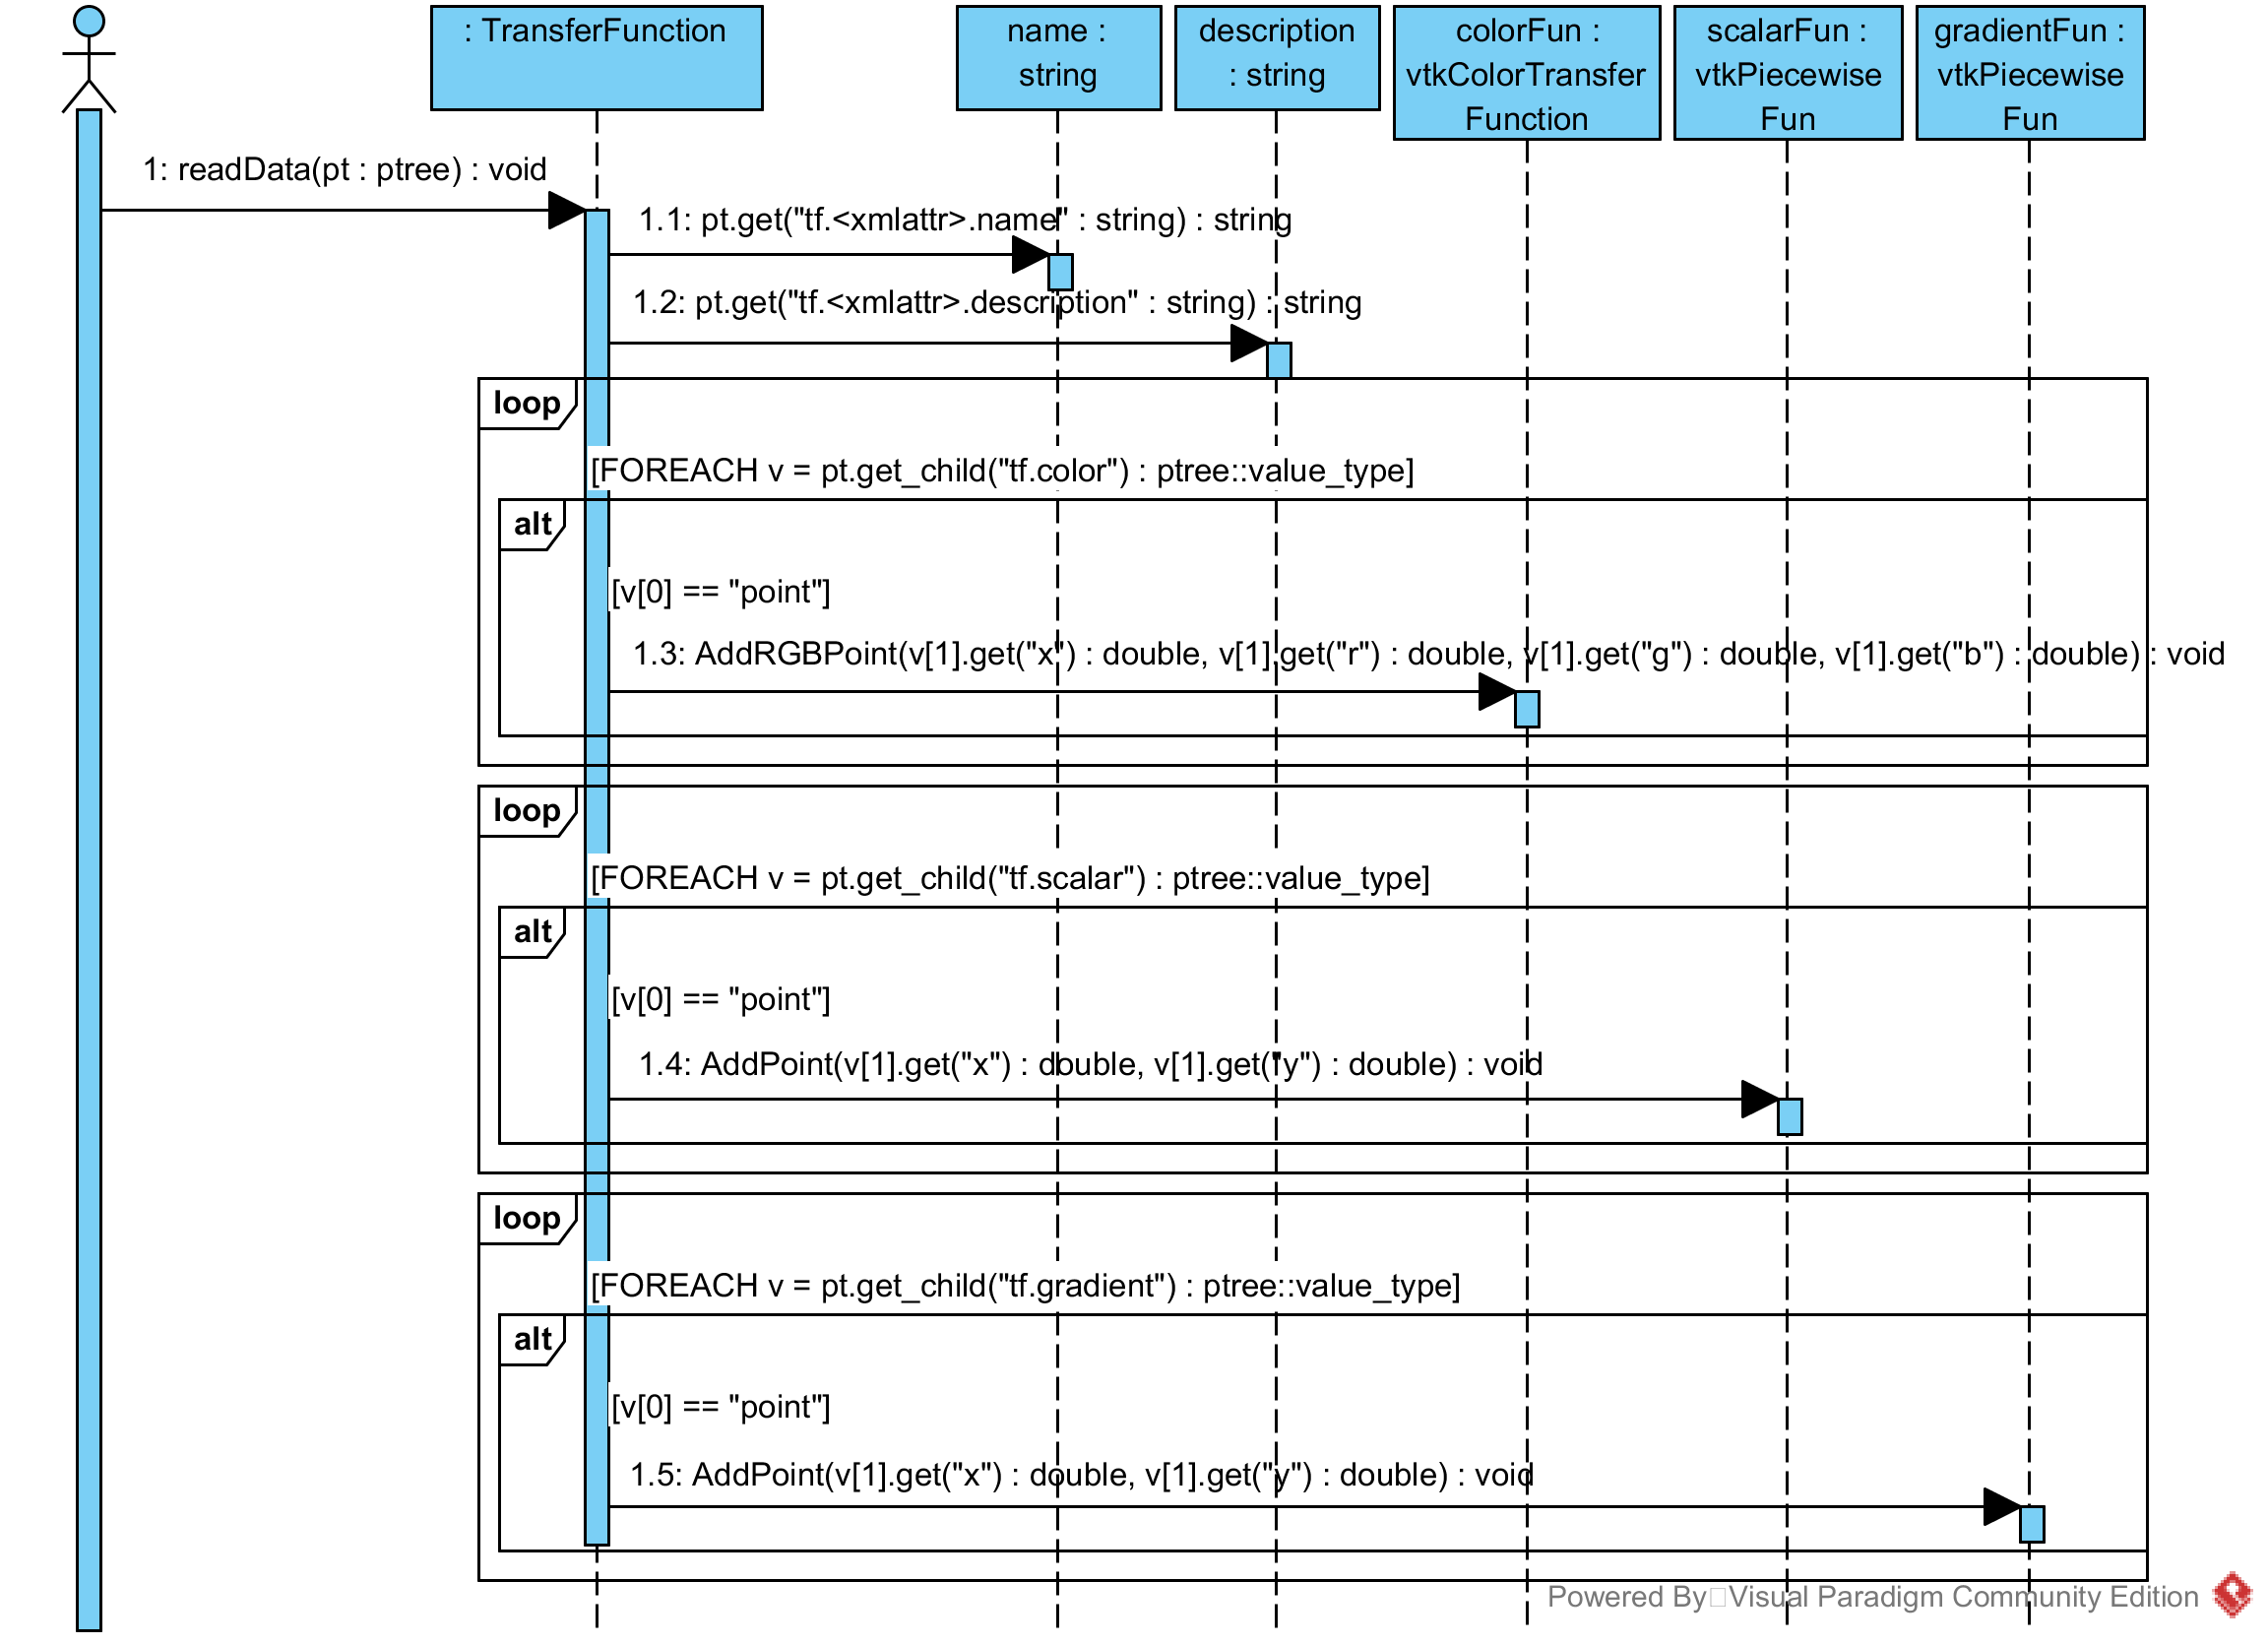
\includegraphics[width=12cm]{imagenes/diagramas/secuencia/TransferFunction_ReadData}
	\caption{Diagrama de secuencia del método \textit{readData} de \textit{TransferFunction}}
	\label{fig:diagrama_secuencia_transferfunction_readdata}
\end{figure}

\begin{figure}[H]
	\centering
	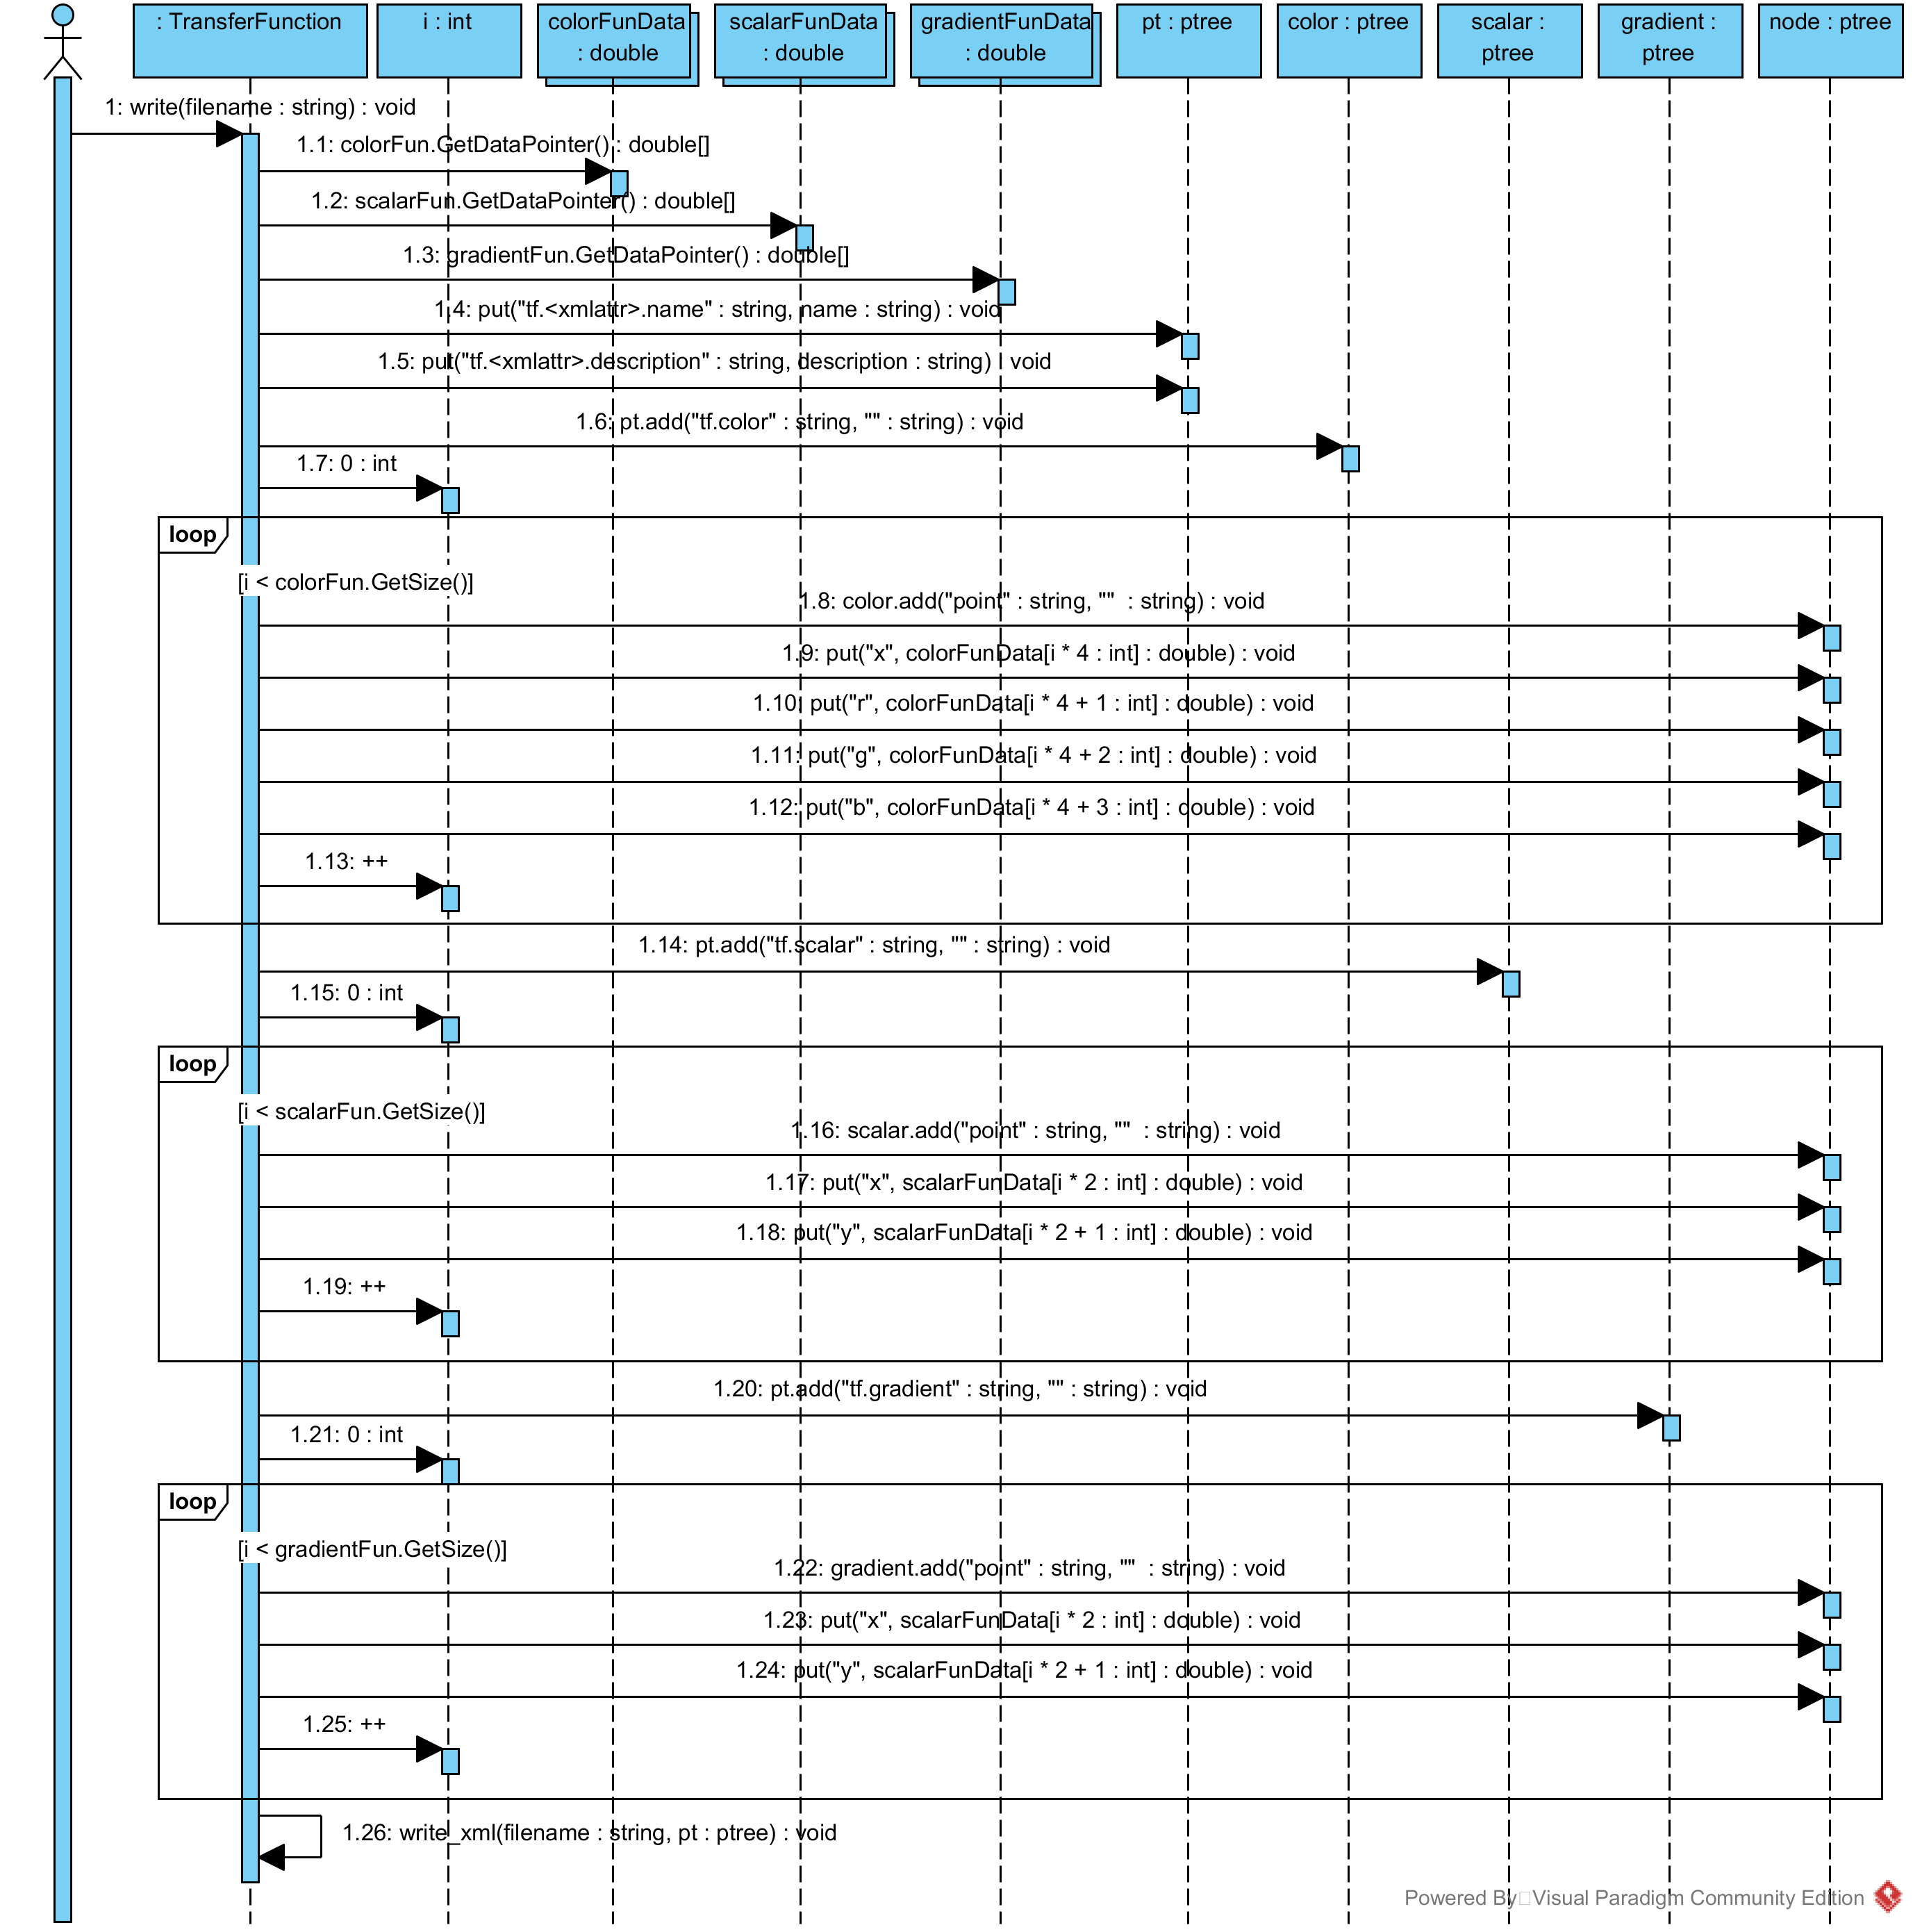
\includegraphics[width=12cm]{imagenes/diagramas/secuencia/TransferFunction_Write}
	\caption{Diagrama de secuencia del método \textit{write} de \textit{TransferFunction}}
	\label{fig:diagrama_secuencia_transferfunction_write}
\end{figure}

\subsection{MainWindow}

\begin{figure}[H]
	\centering
	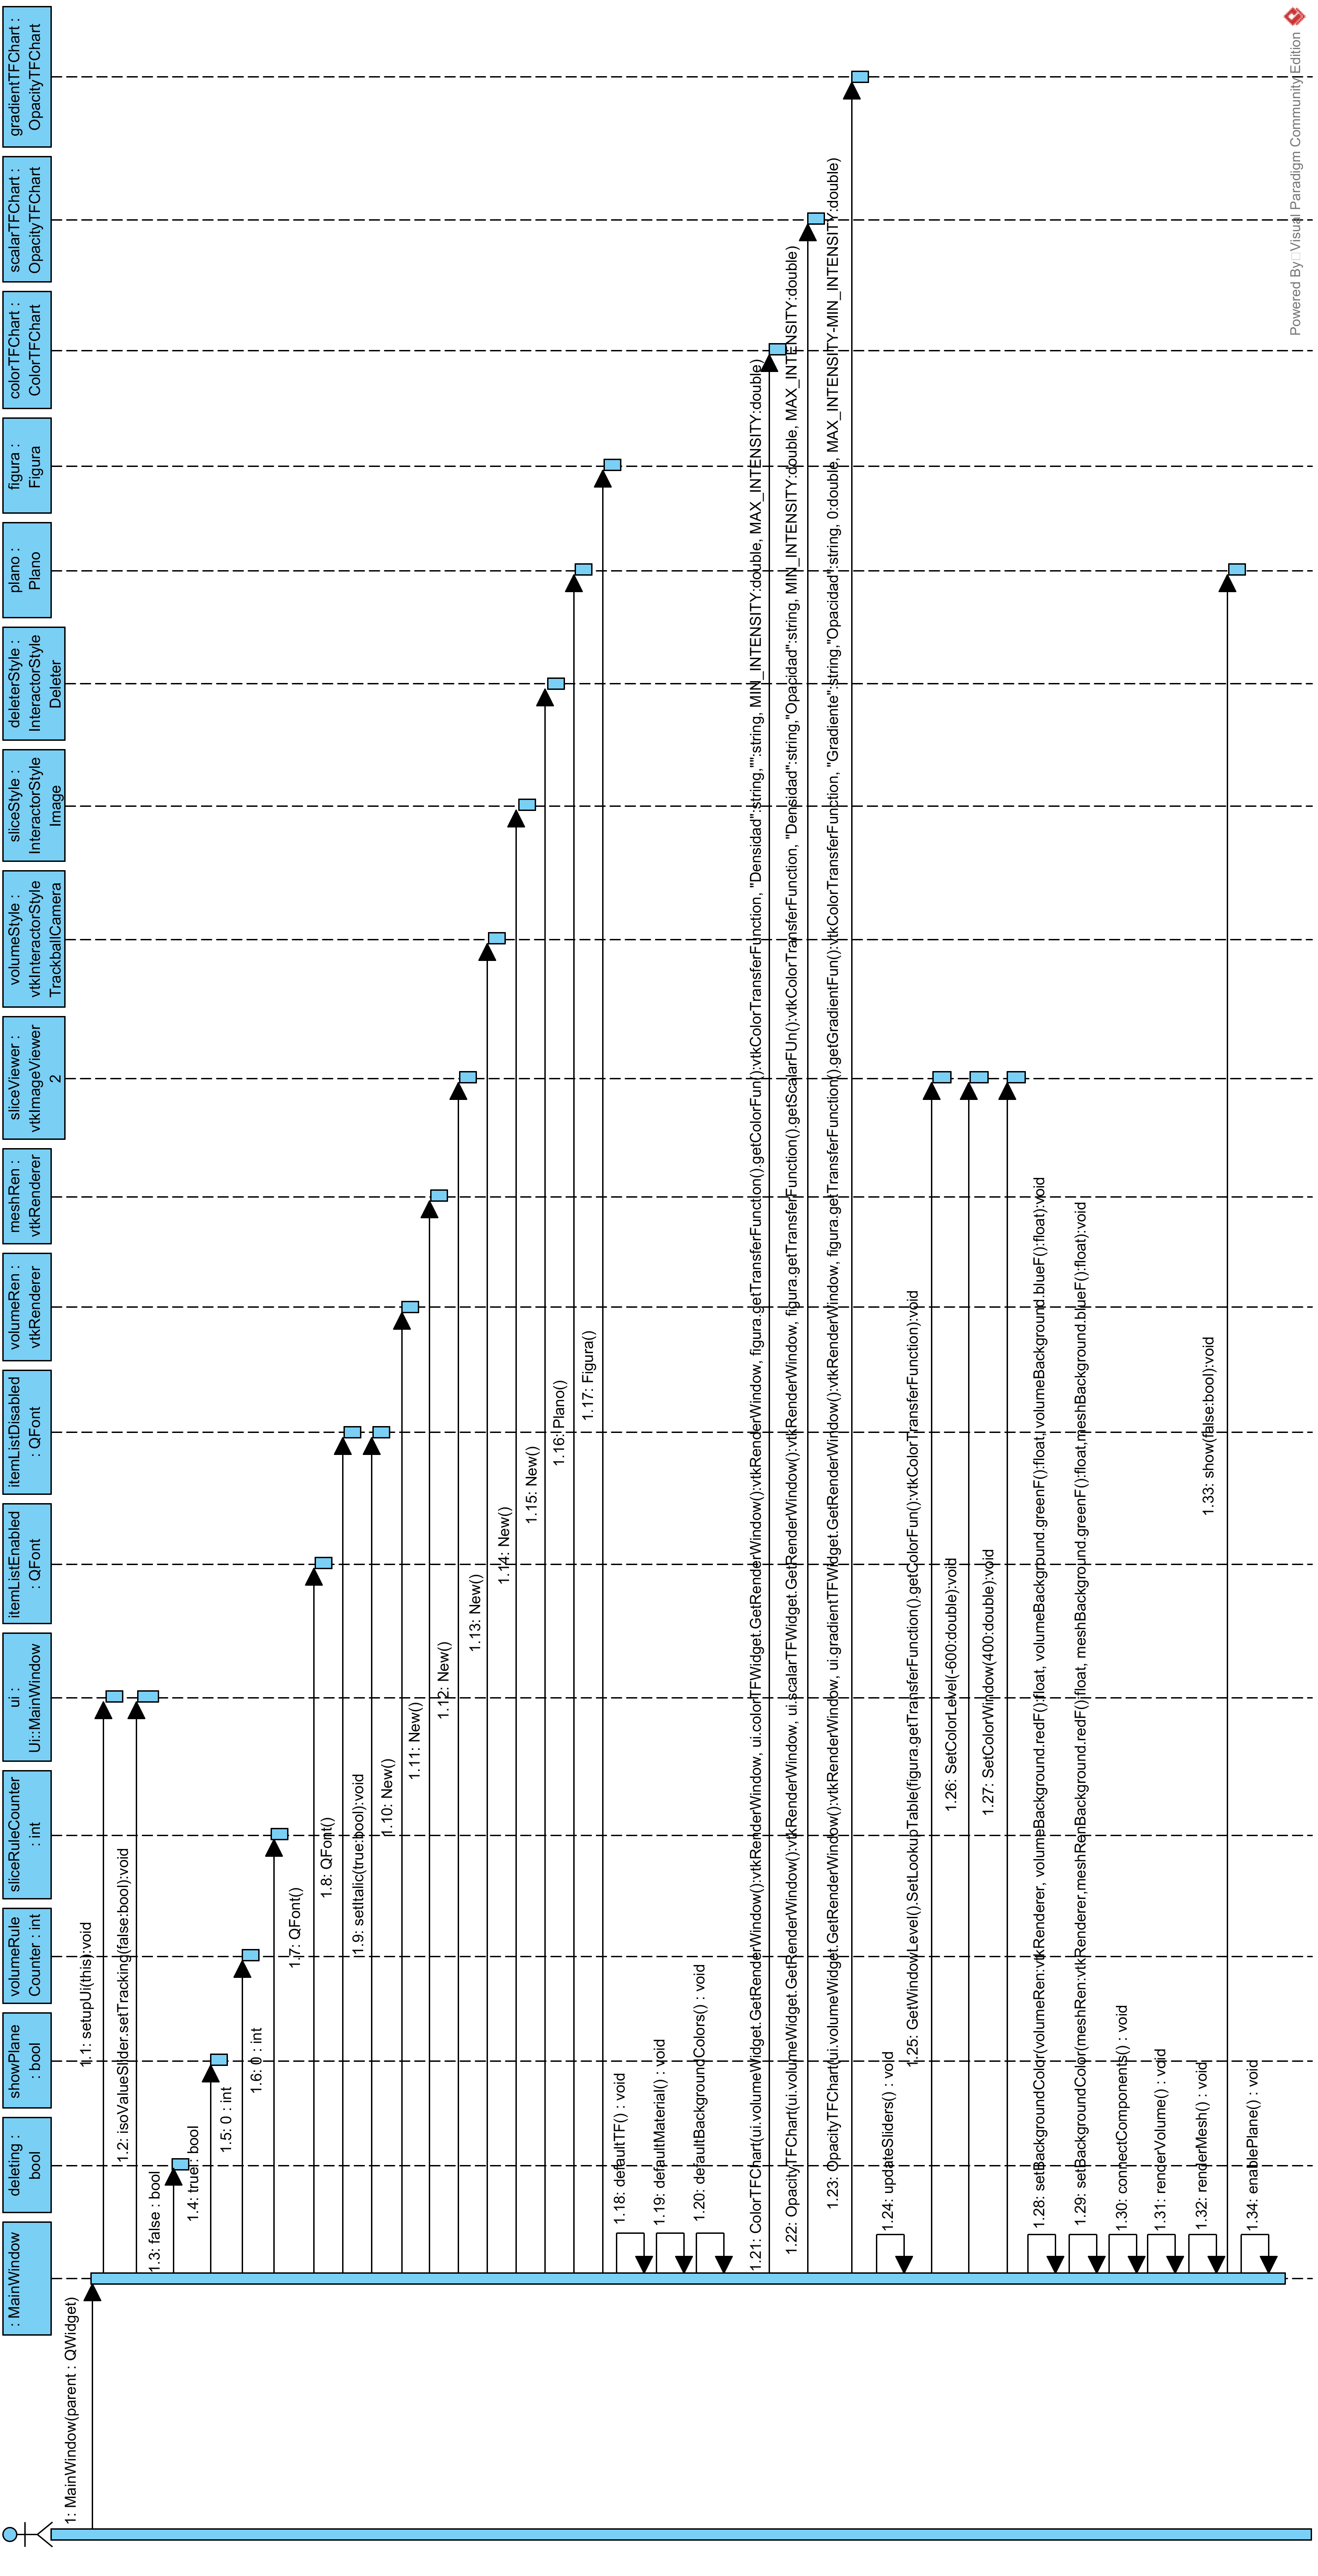
\includegraphics[angle=90,height=18cm]{imagenes/diagramas/secuencia/MainWindow_New}
	\caption{Diagrama de secuencia del constructor de \textit{MainWindow}}
	\label{fig:diagrama_secuencia_mainwindow_new}
\end{figure}

\begin{figure}[H]
	\centering
	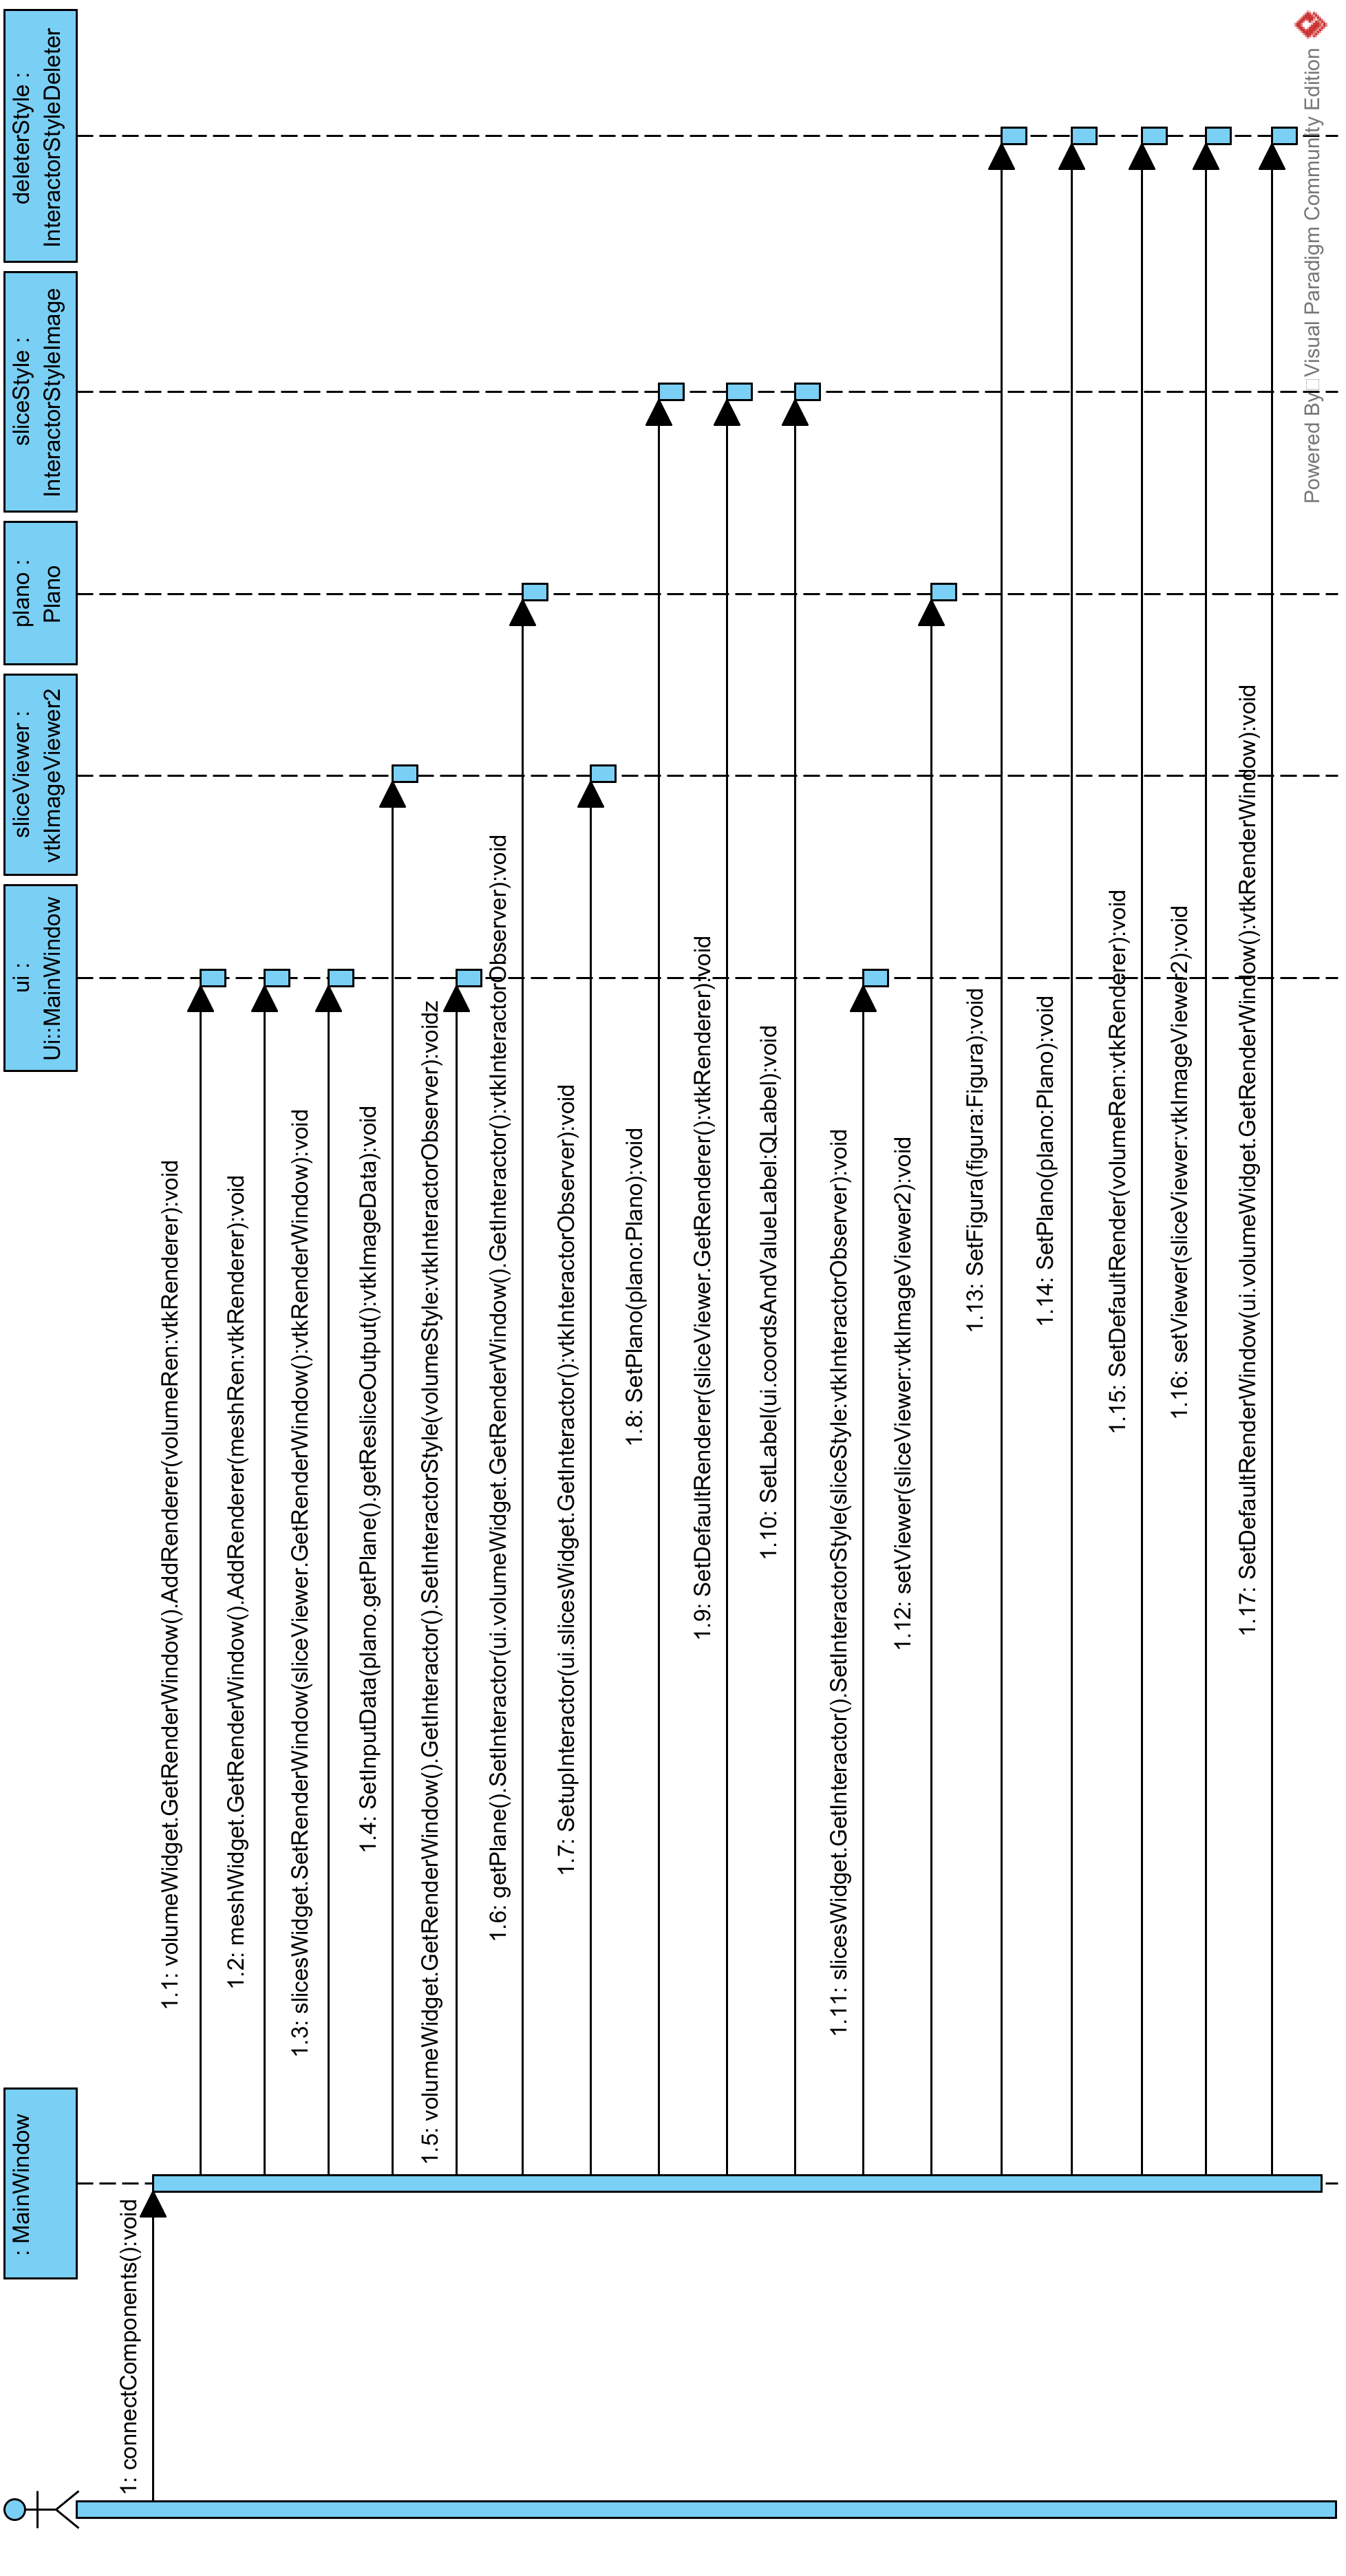
\includegraphics[angle=90,height=18cm]{imagenes/diagramas/secuencia/MainWindow_ConnectComponents}
	\caption{Diagrama de secuencia del método \textit{connectComponents} de \textit{MainWindow}}
	\label{fig:diagrama_secuencia_mainwindow_connectcomponents}
\end{figure}

\begin{figure}[H]
	\centering
	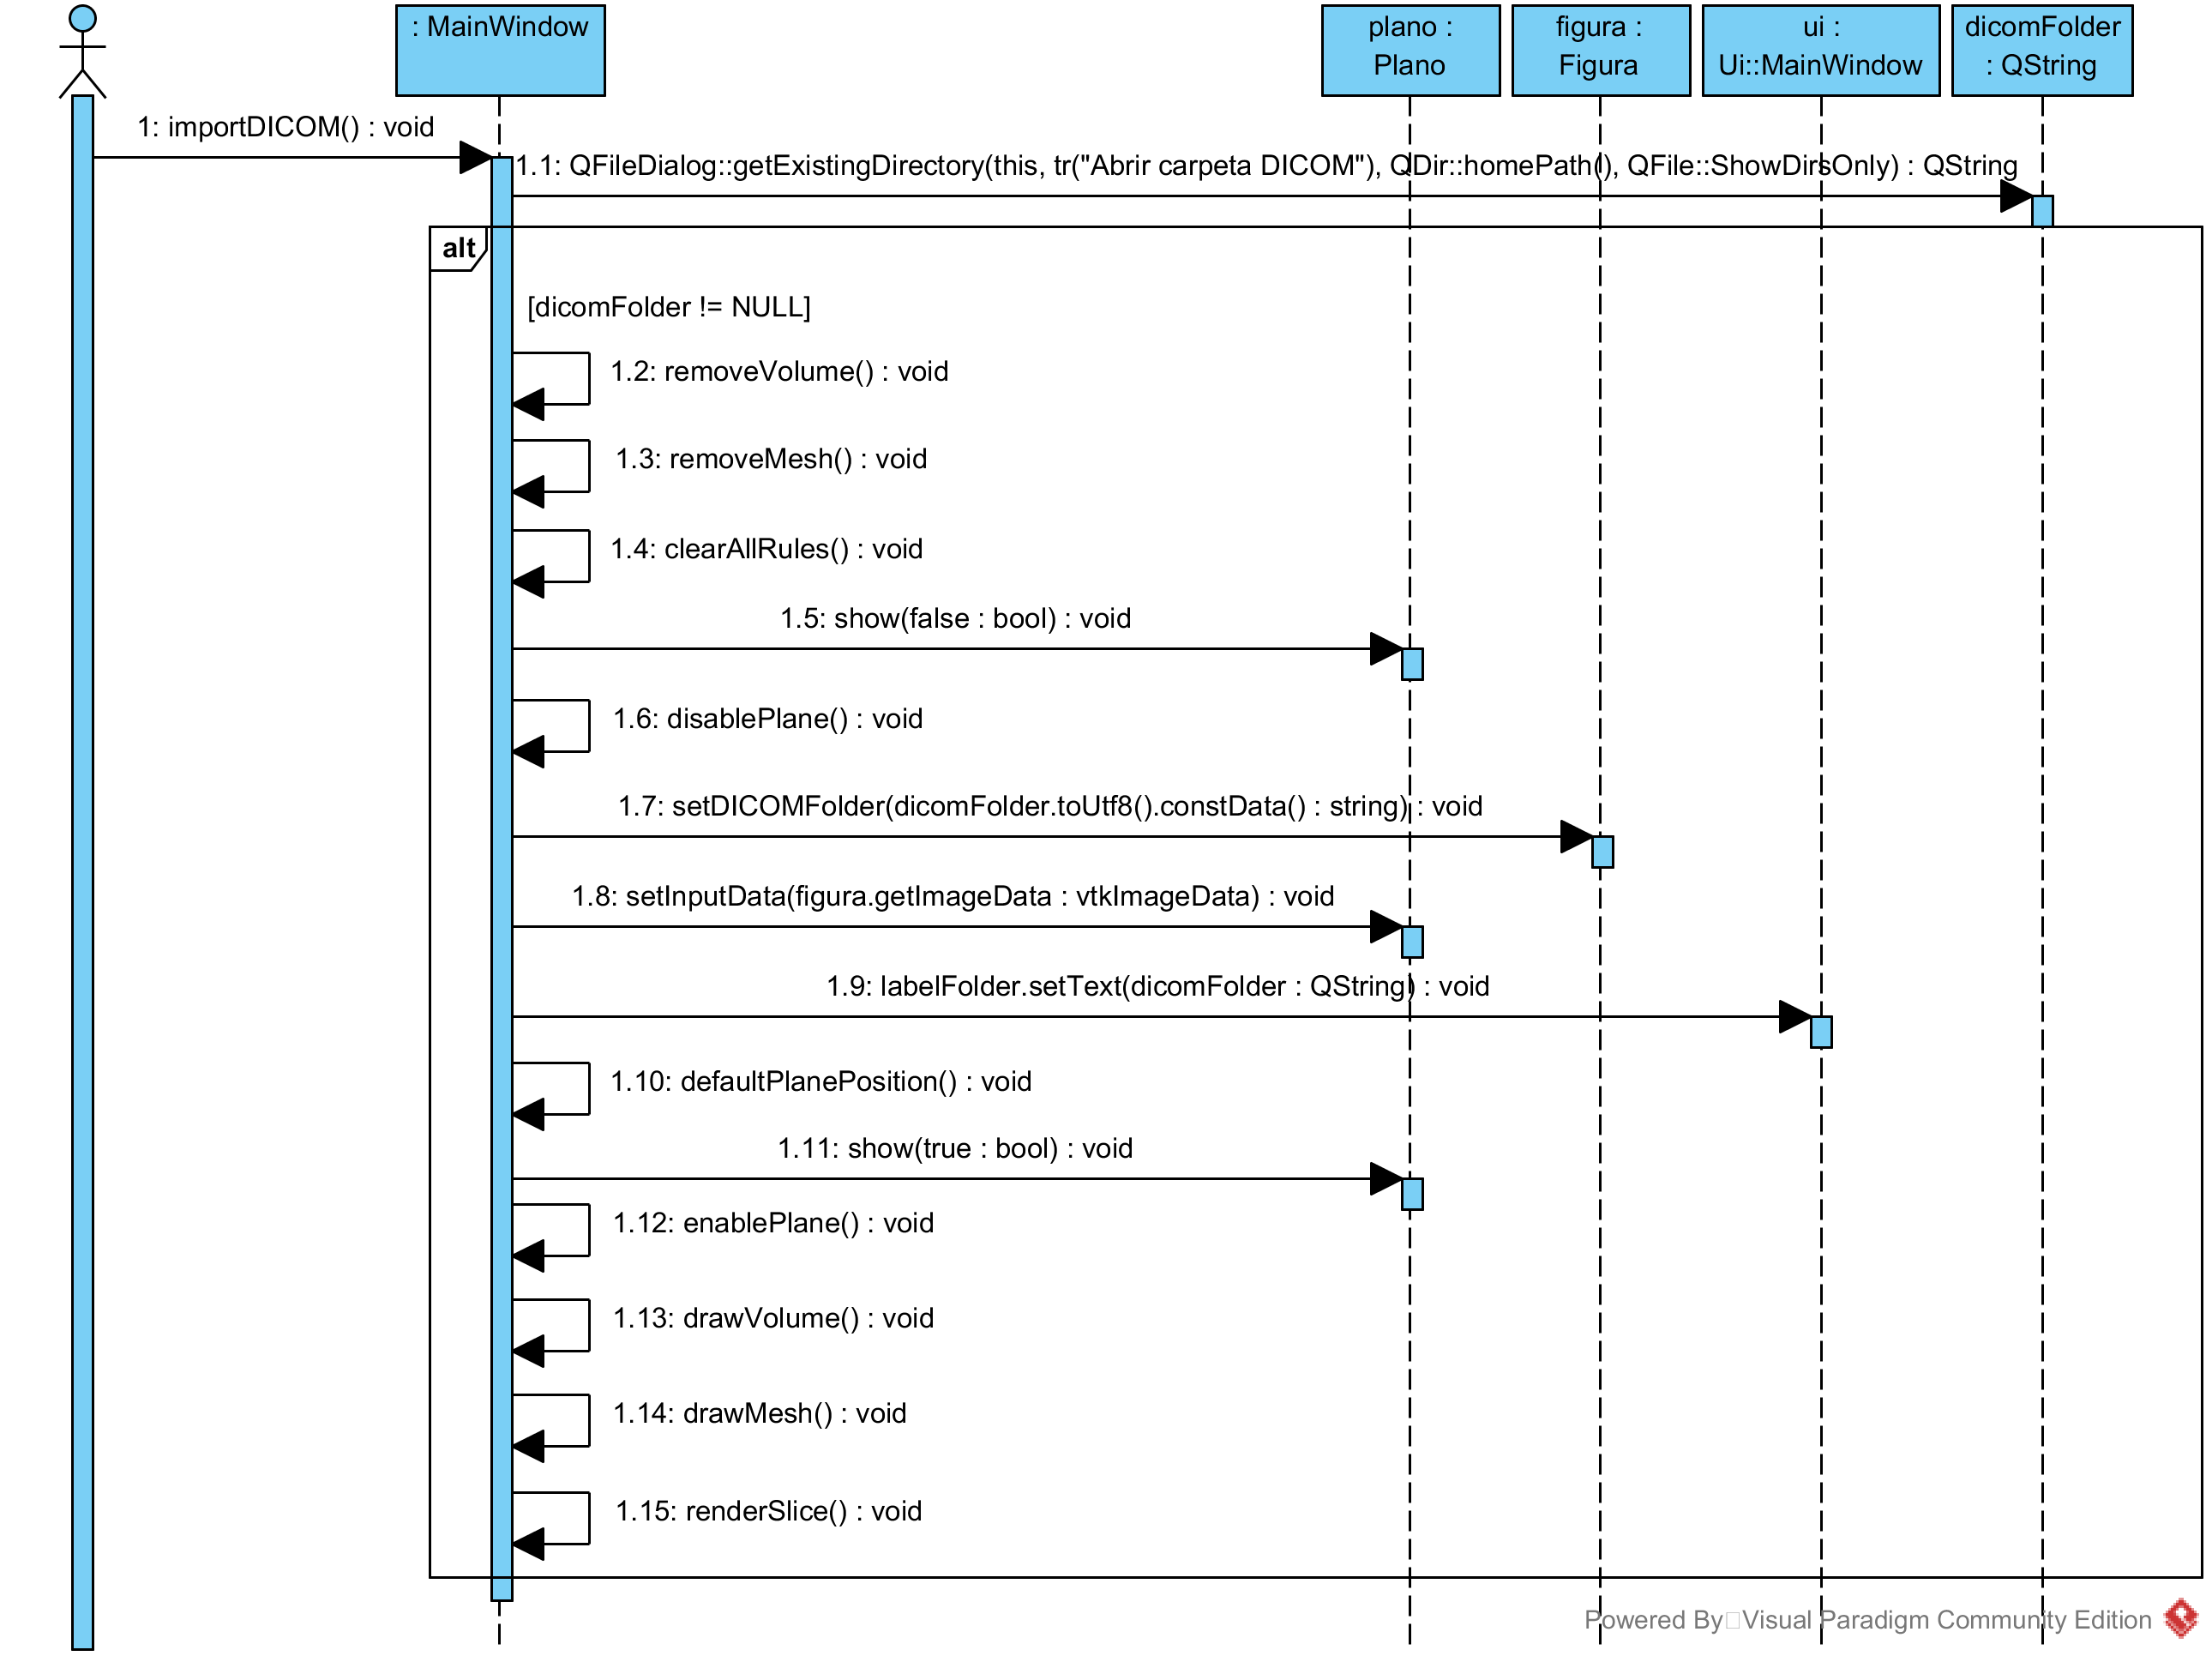
\includegraphics[angle=90,height=18cm]{imagenes/diagramas/secuencia/MainWindow_ImportDICOM}
	\caption{Diagrama de secuencia del método \textit{importDICOM} de \textit{MainWindow}}
	\label{fig:diagrama_secuencia_mainwindow_importdicom}
\end{figure}

\begin{figure}[H]
	\centering
	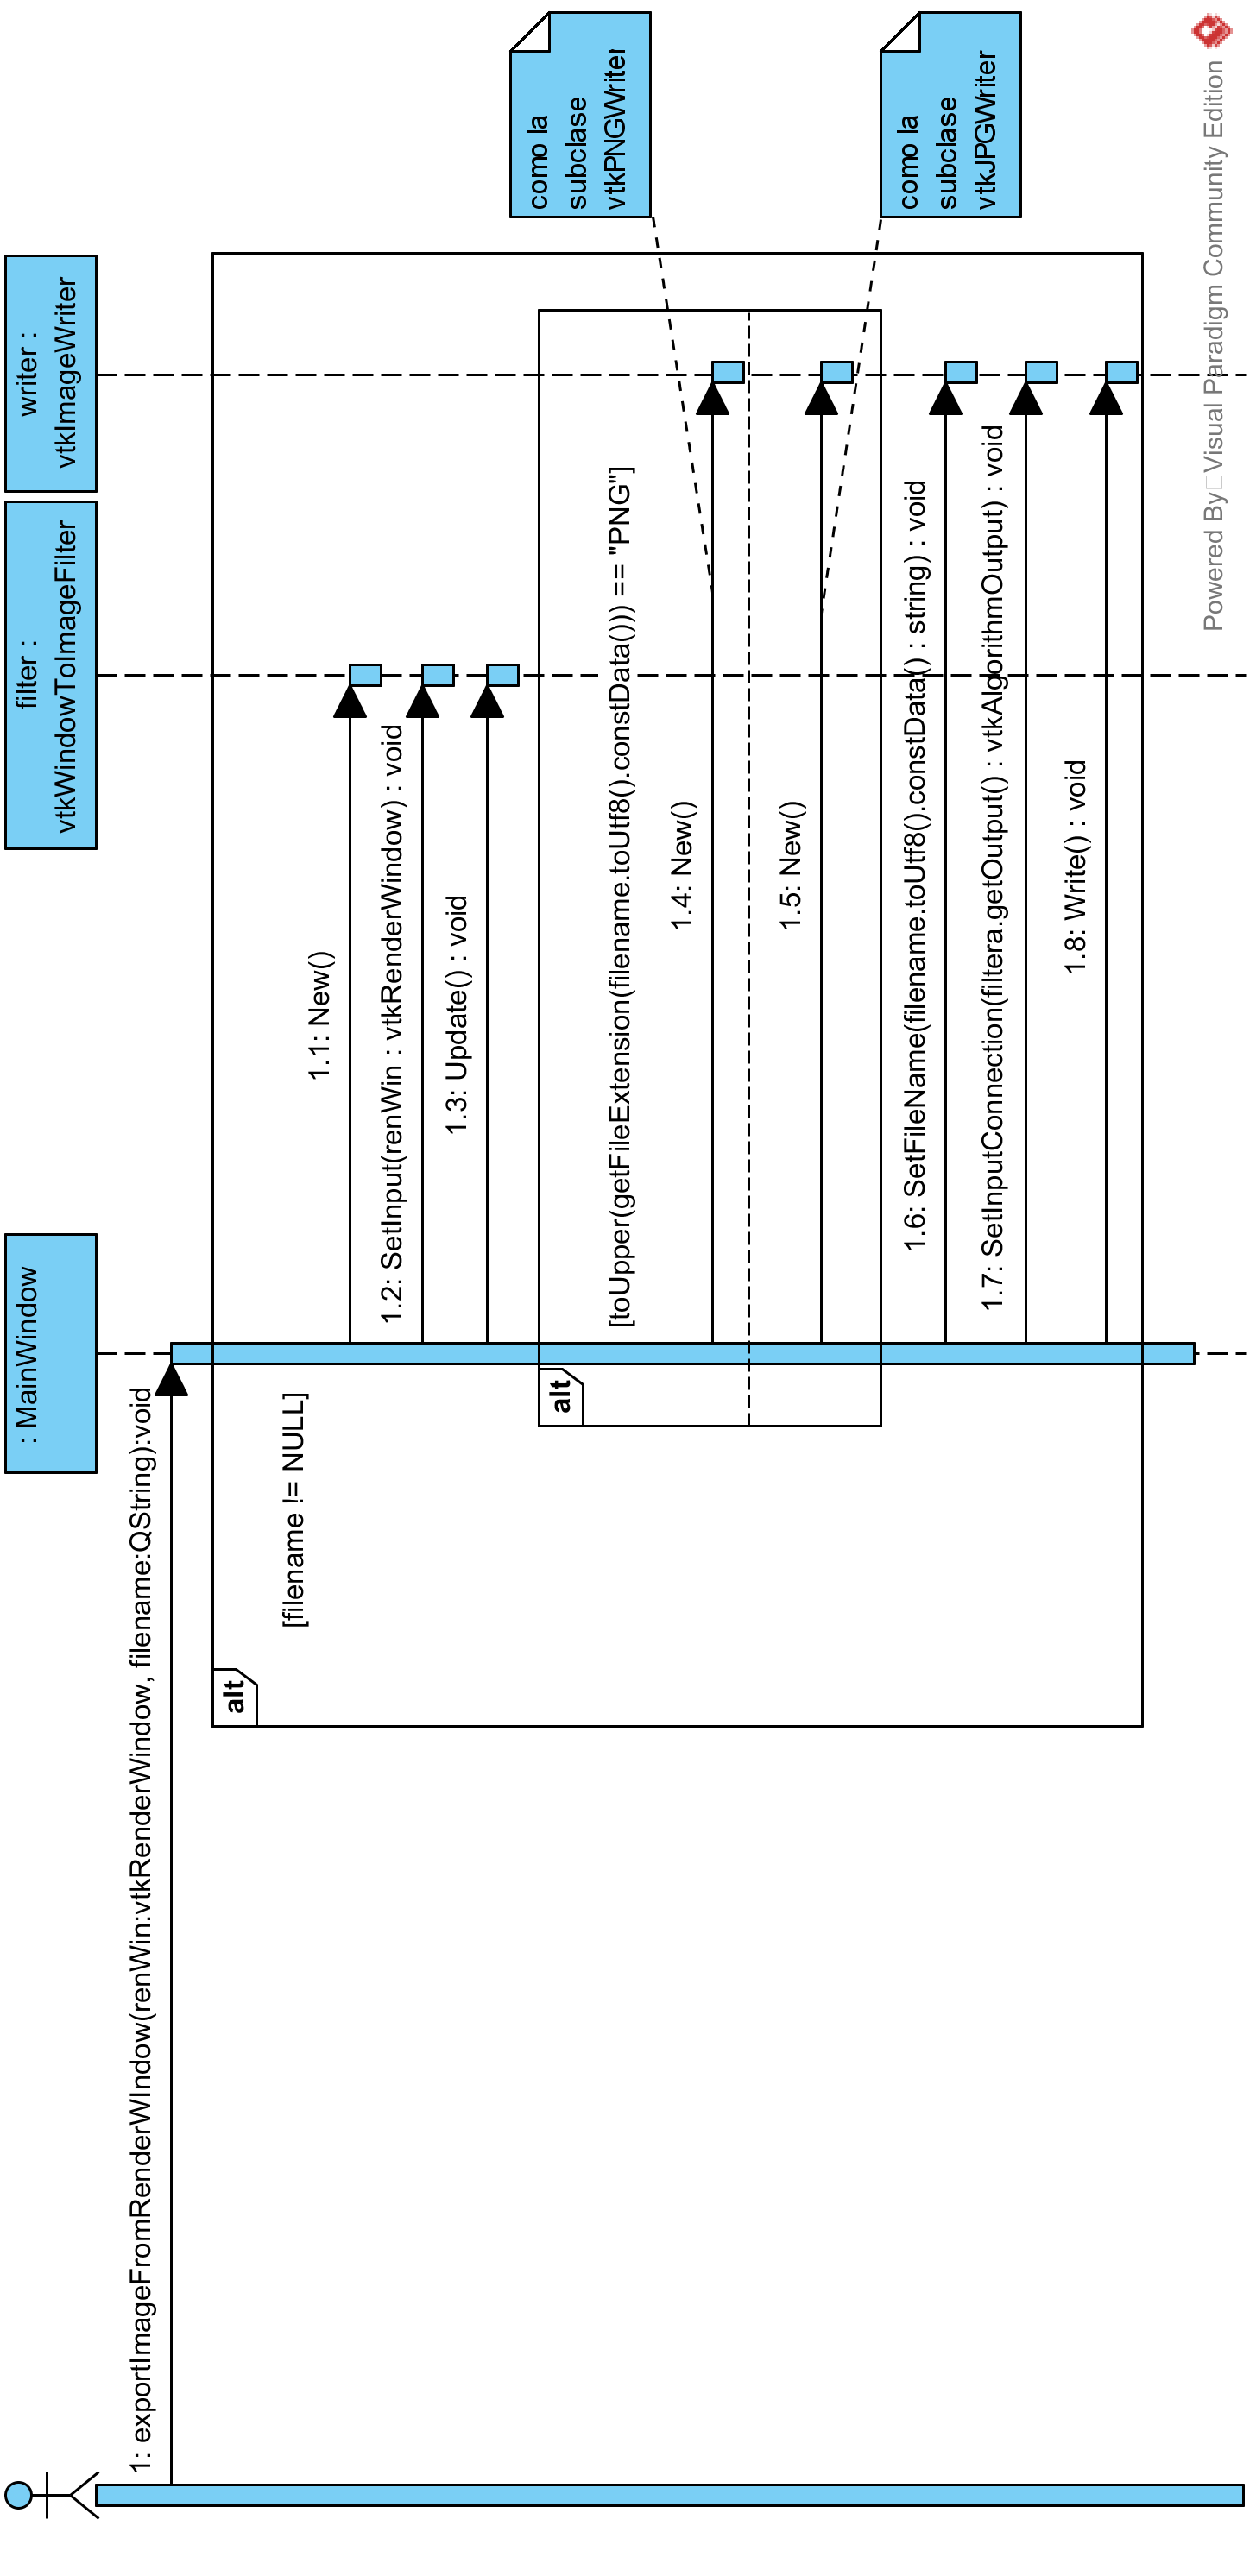
\includegraphics[angle=90,height=18cm]{imagenes/diagramas/secuencia/MainWindow_ExportImageFromRenderWindow}
	\caption{Diagrama de secuencia del método \textit{exportImageFromRenderWindow} de \textit{MainWindow}}
	\label{fig:diagrama_secuencia_mainwindow_exportimagefromrenderwindow}
\end{figure}

\begin{figure}[H]
	\centering
	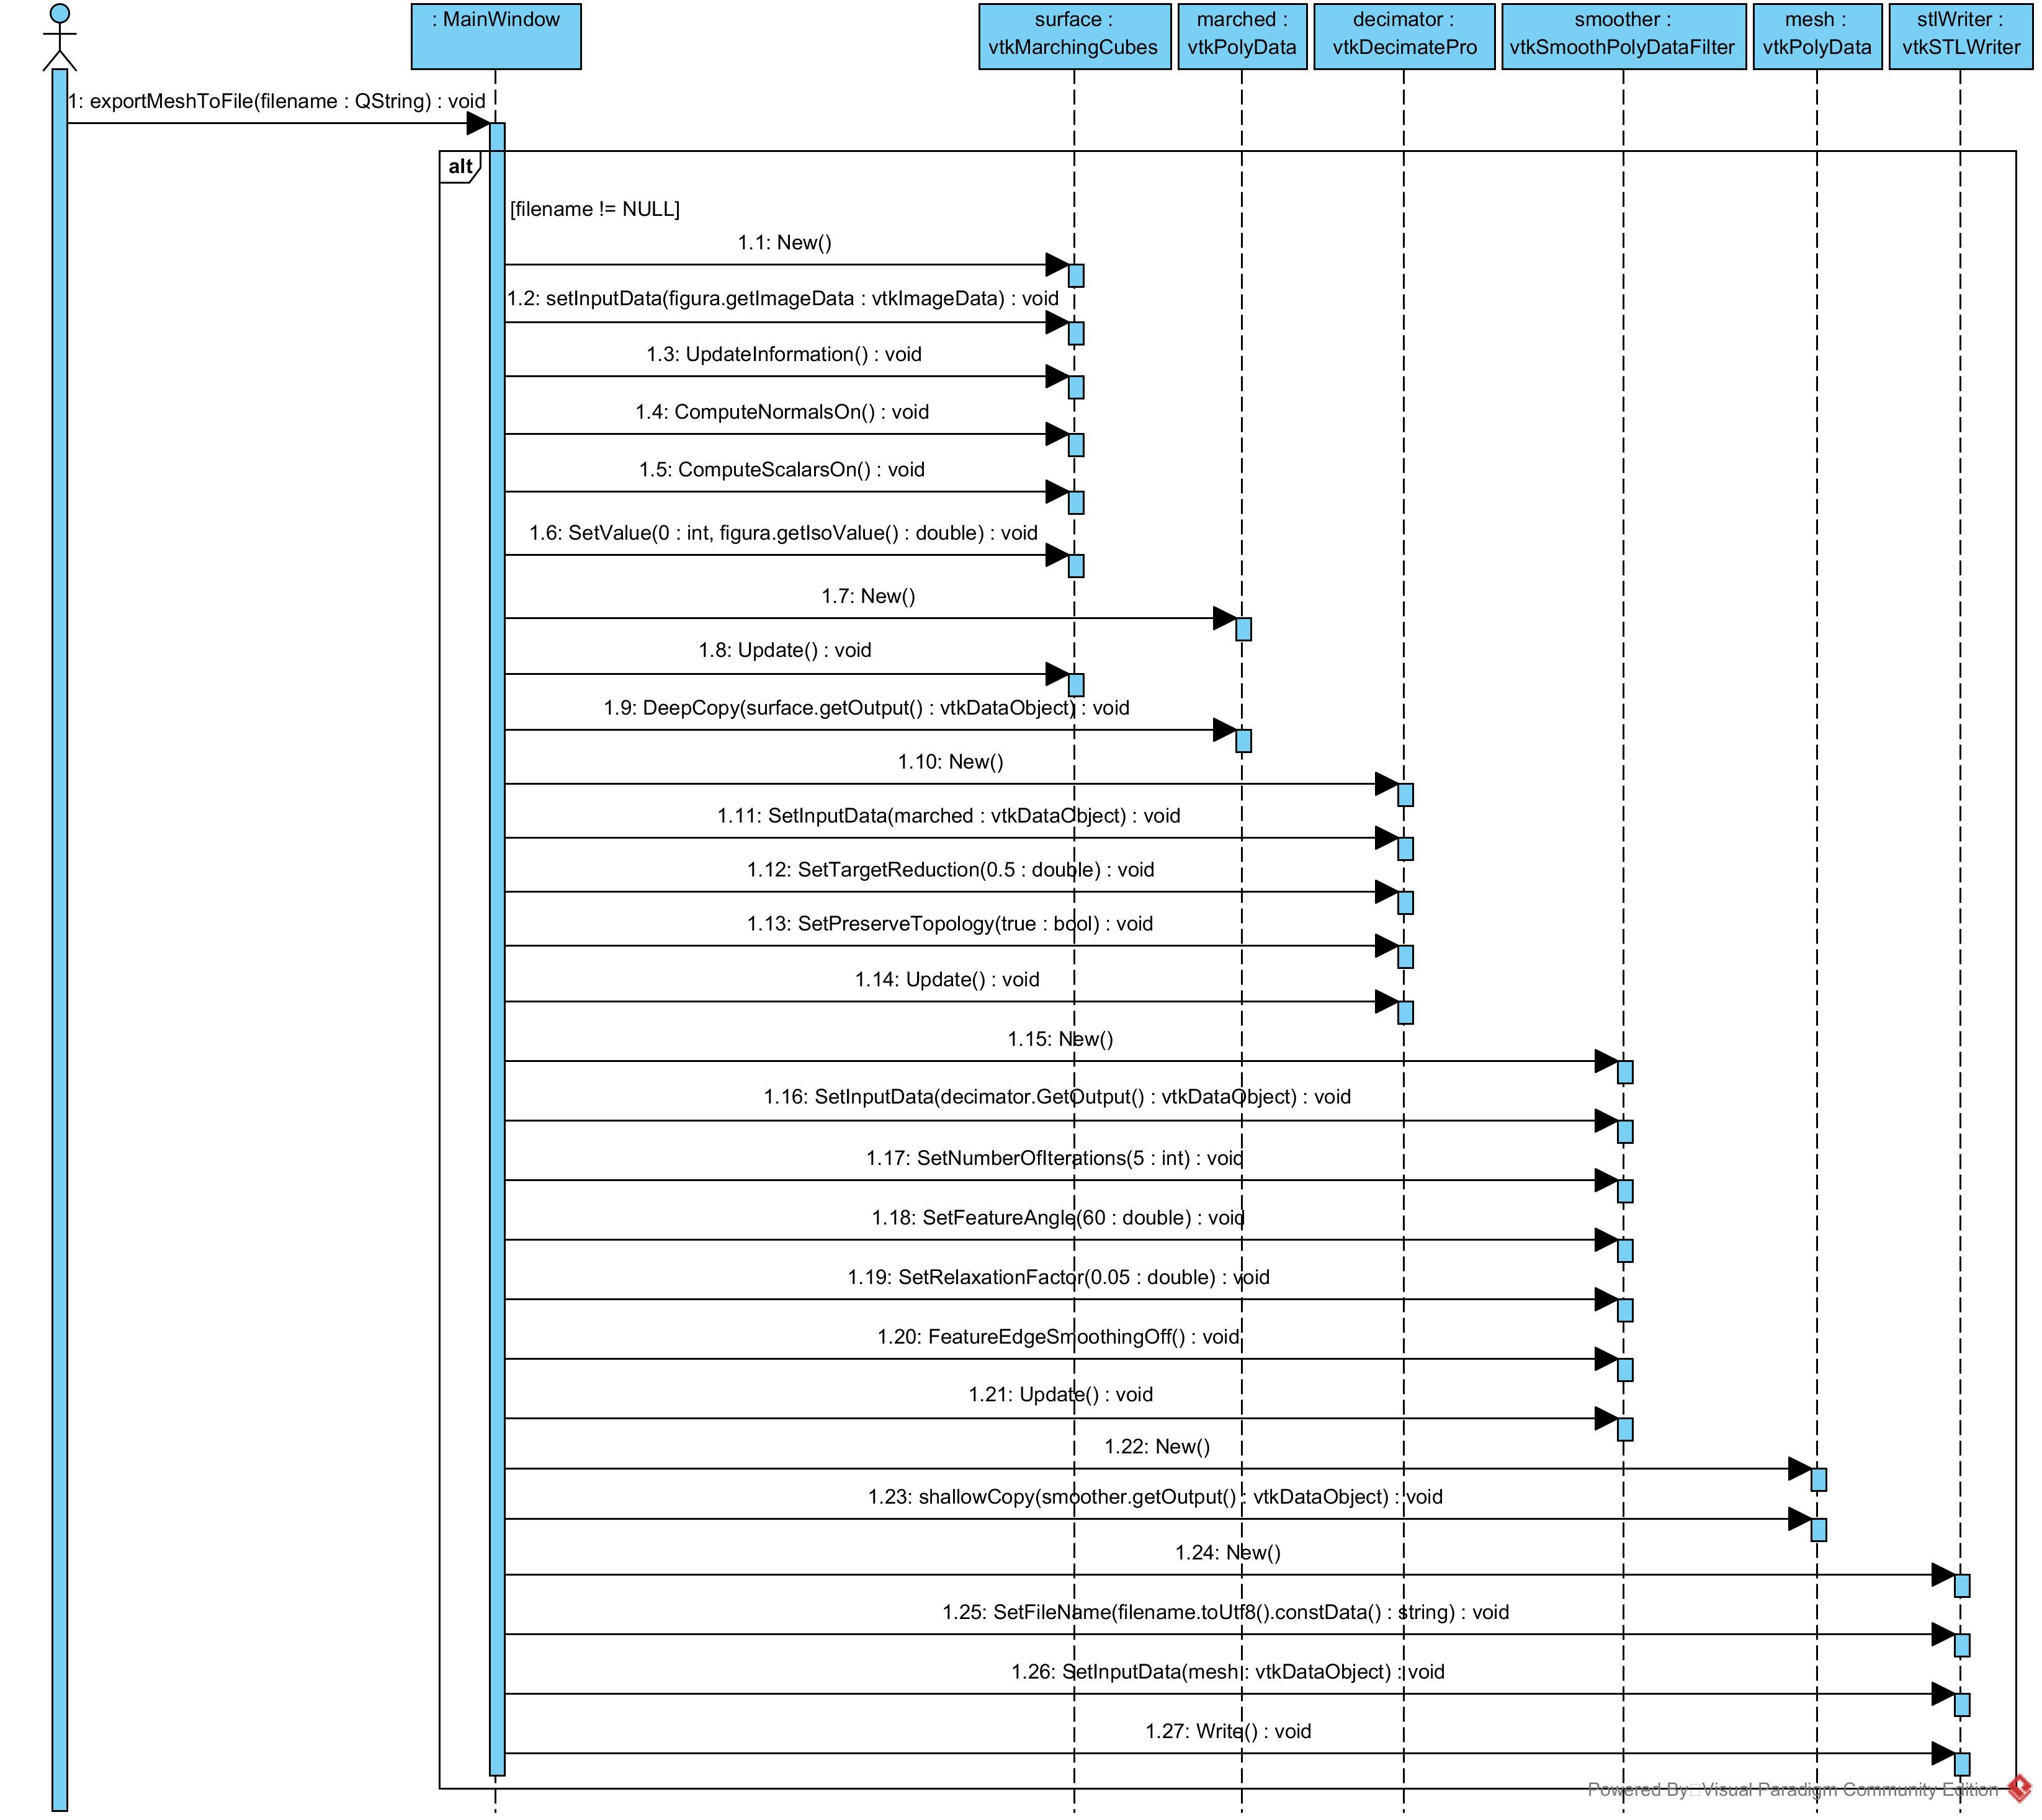
\includegraphics[angle=90,width=12cm]{imagenes/diagramas/secuencia/MainWindow_ExportMeshToFile}
	\caption{Diagrama de secuencia del método \textit{exportMeshToFile} de \textit{MainWindow}}
	\label{fig:diagrama_secuencia_mainwindow_exportmeshtofile}
\end{figure}

\begin{figure}[H]
	\centering
	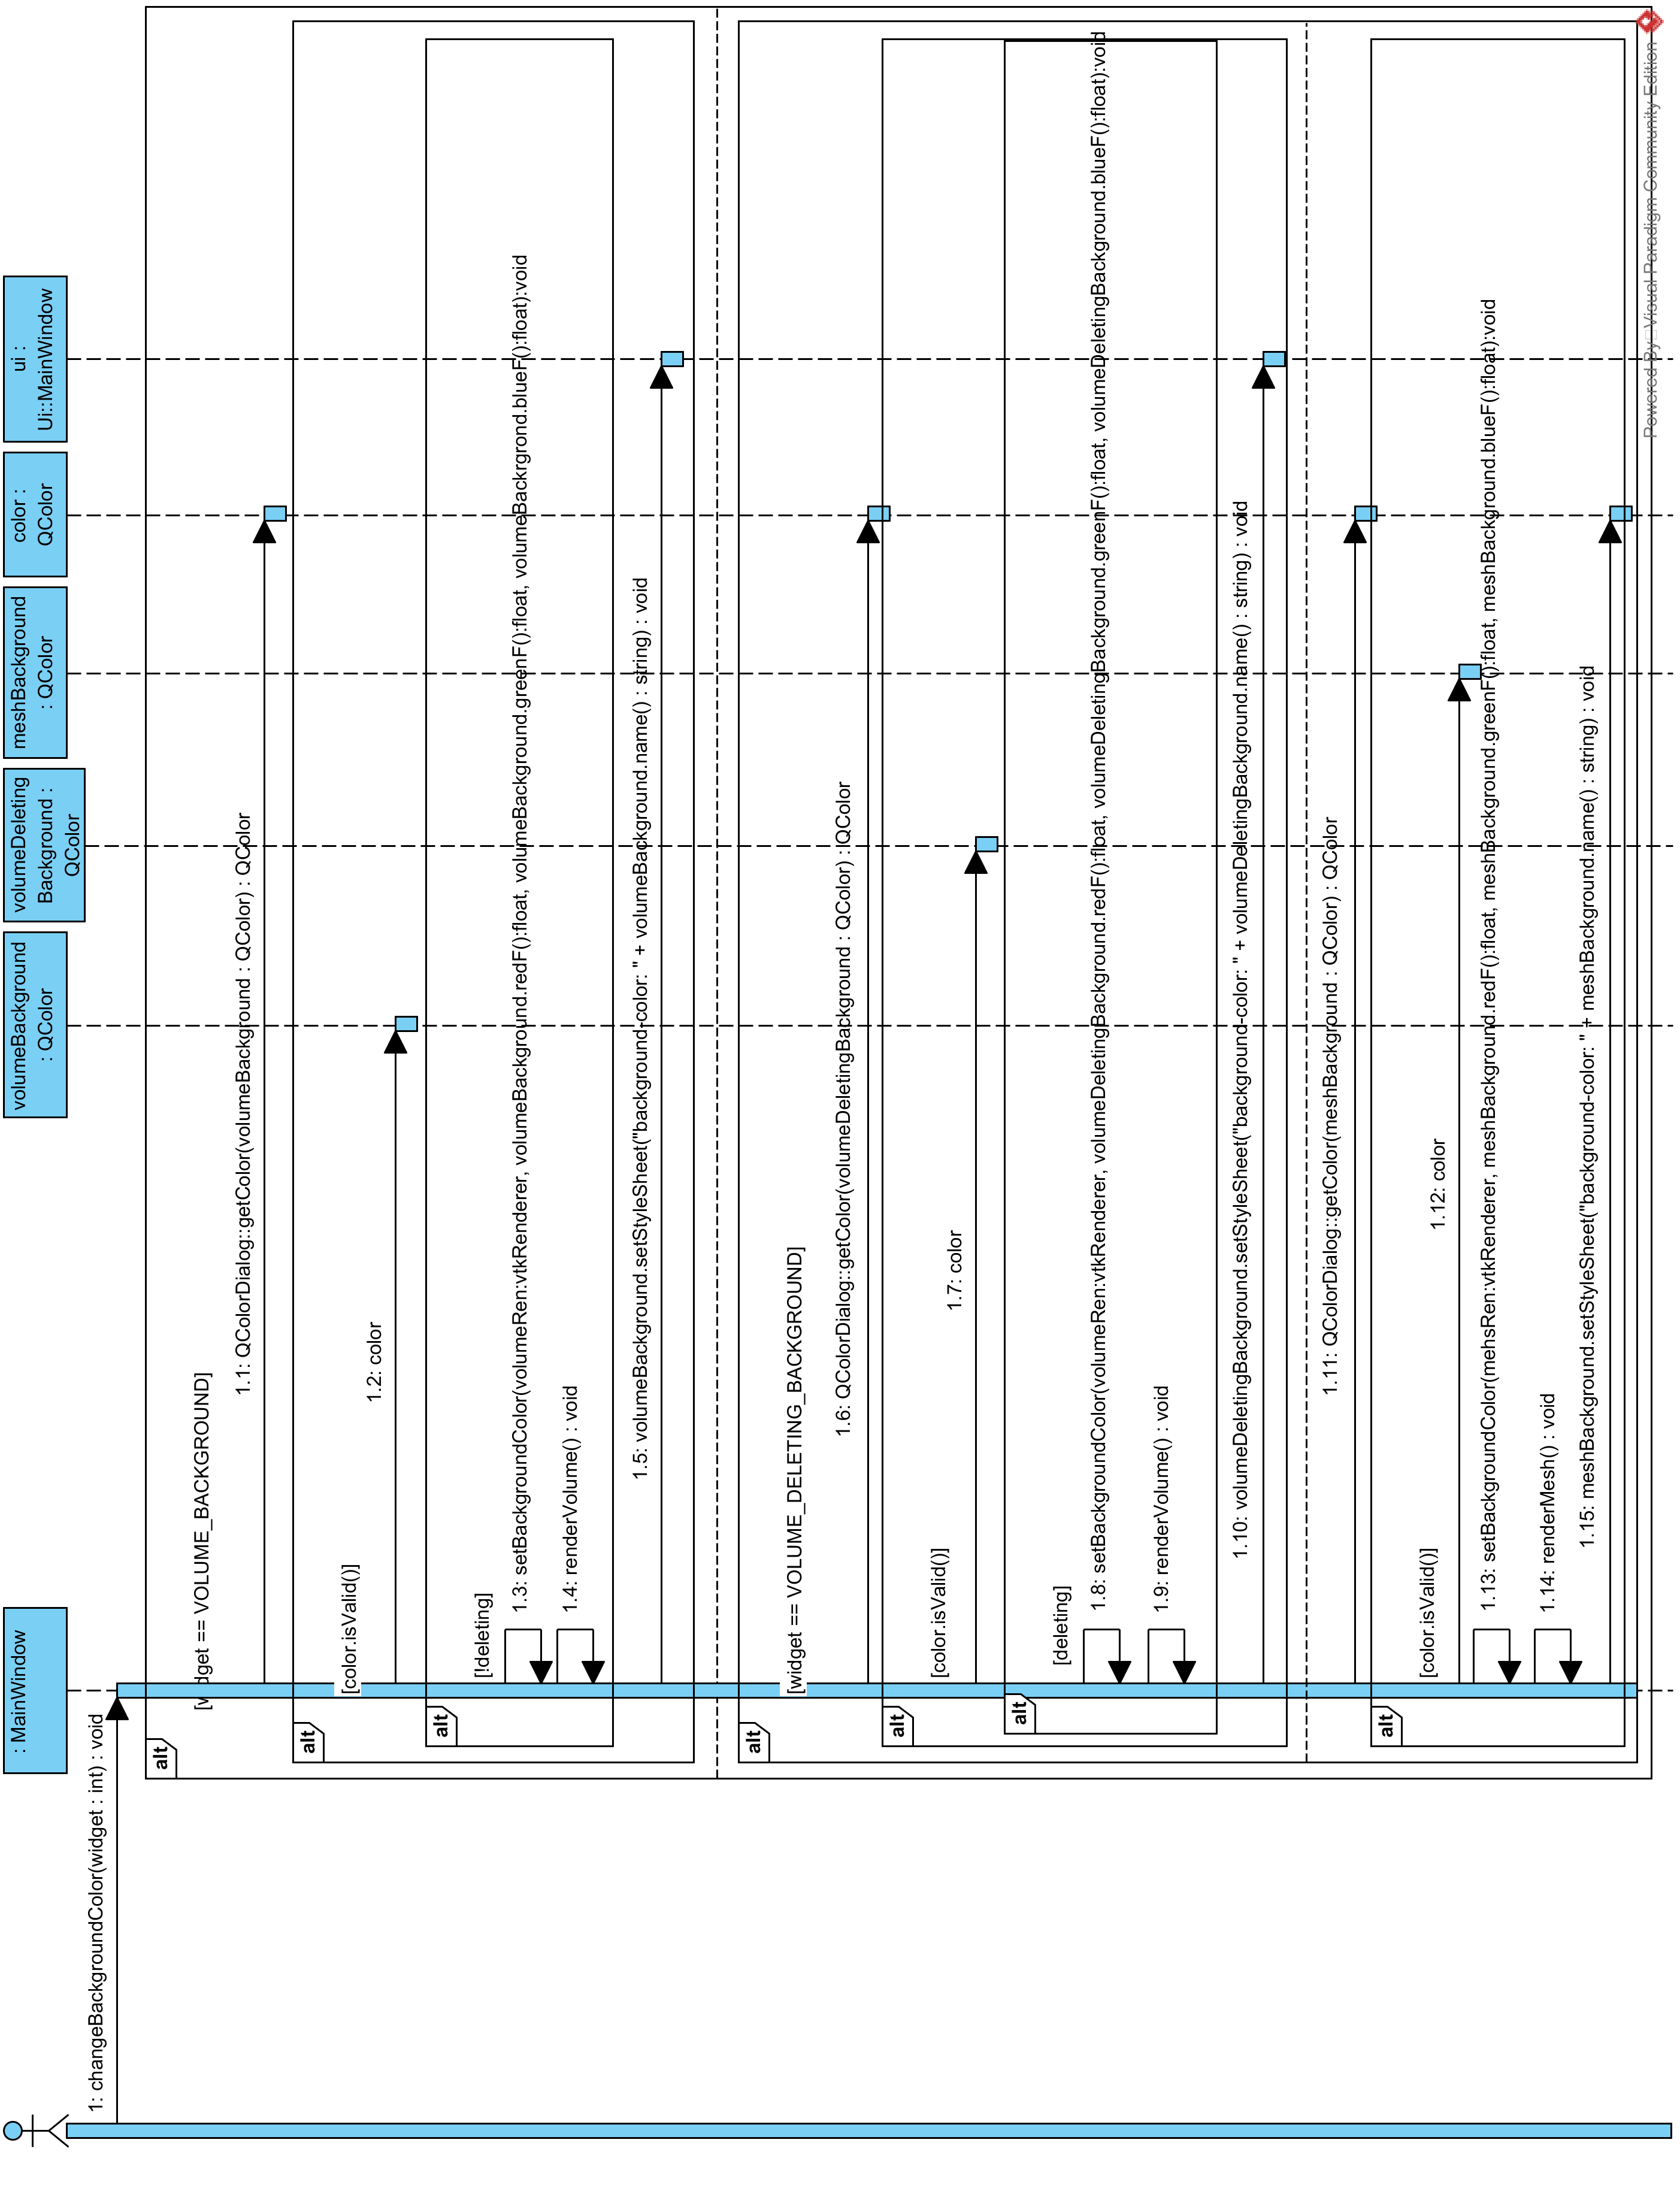
\includegraphics[angle=90,width=12cm]{imagenes/diagramas/secuencia/MainWindow_ChangeBackgroundColor}
	\caption{Diagrama de secuencia del método \textit{changeBackgroundColor} de \textit{MainWindow}}
	\label{fig:diagrama_secuencia_mainwindow_changeBackgroundColor}
\end{figure}

\begin{figure}[H]
	\centering
	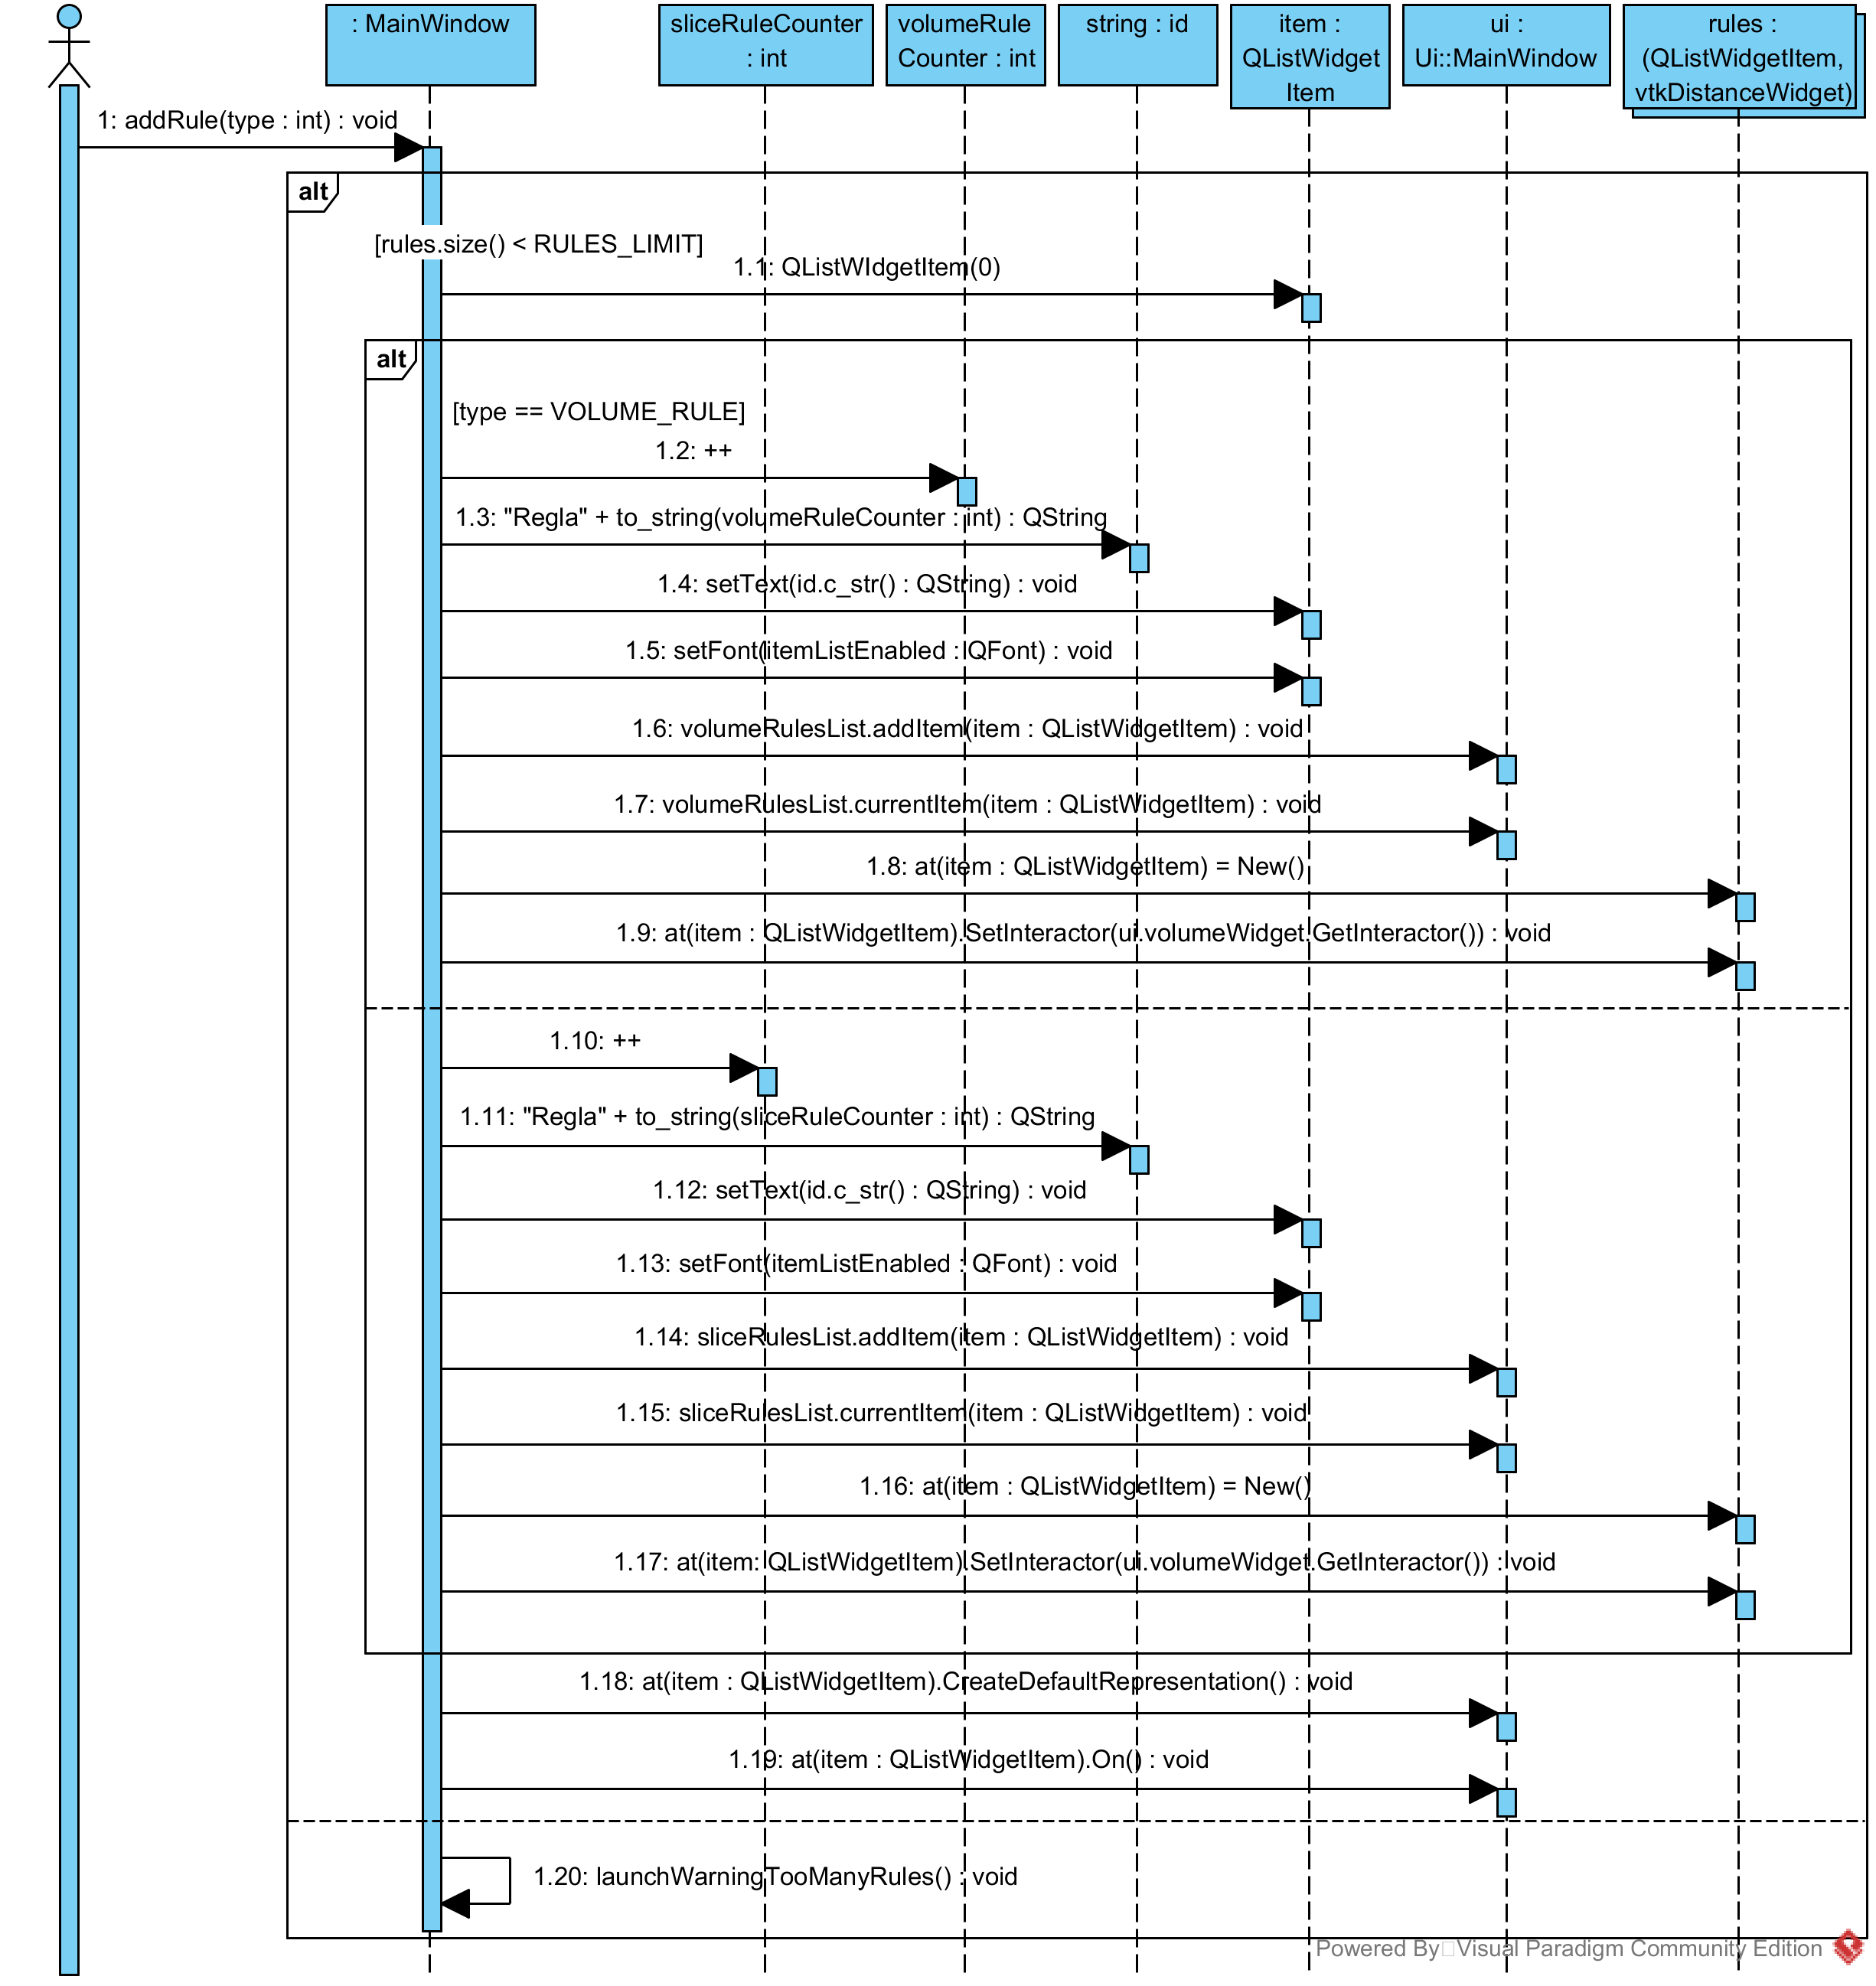
\includegraphics[width=12cm]{imagenes/diagramas/secuencia/MainWindow_AddRule}
	\caption{Diagrama de secuencia del método \textit{addRule} de \textit{MainWindow}}
	\label{fig:diagrama_secuencia_mainwindow_addrule}
\end{figure}

\begin{figure}[H]
	\centering
	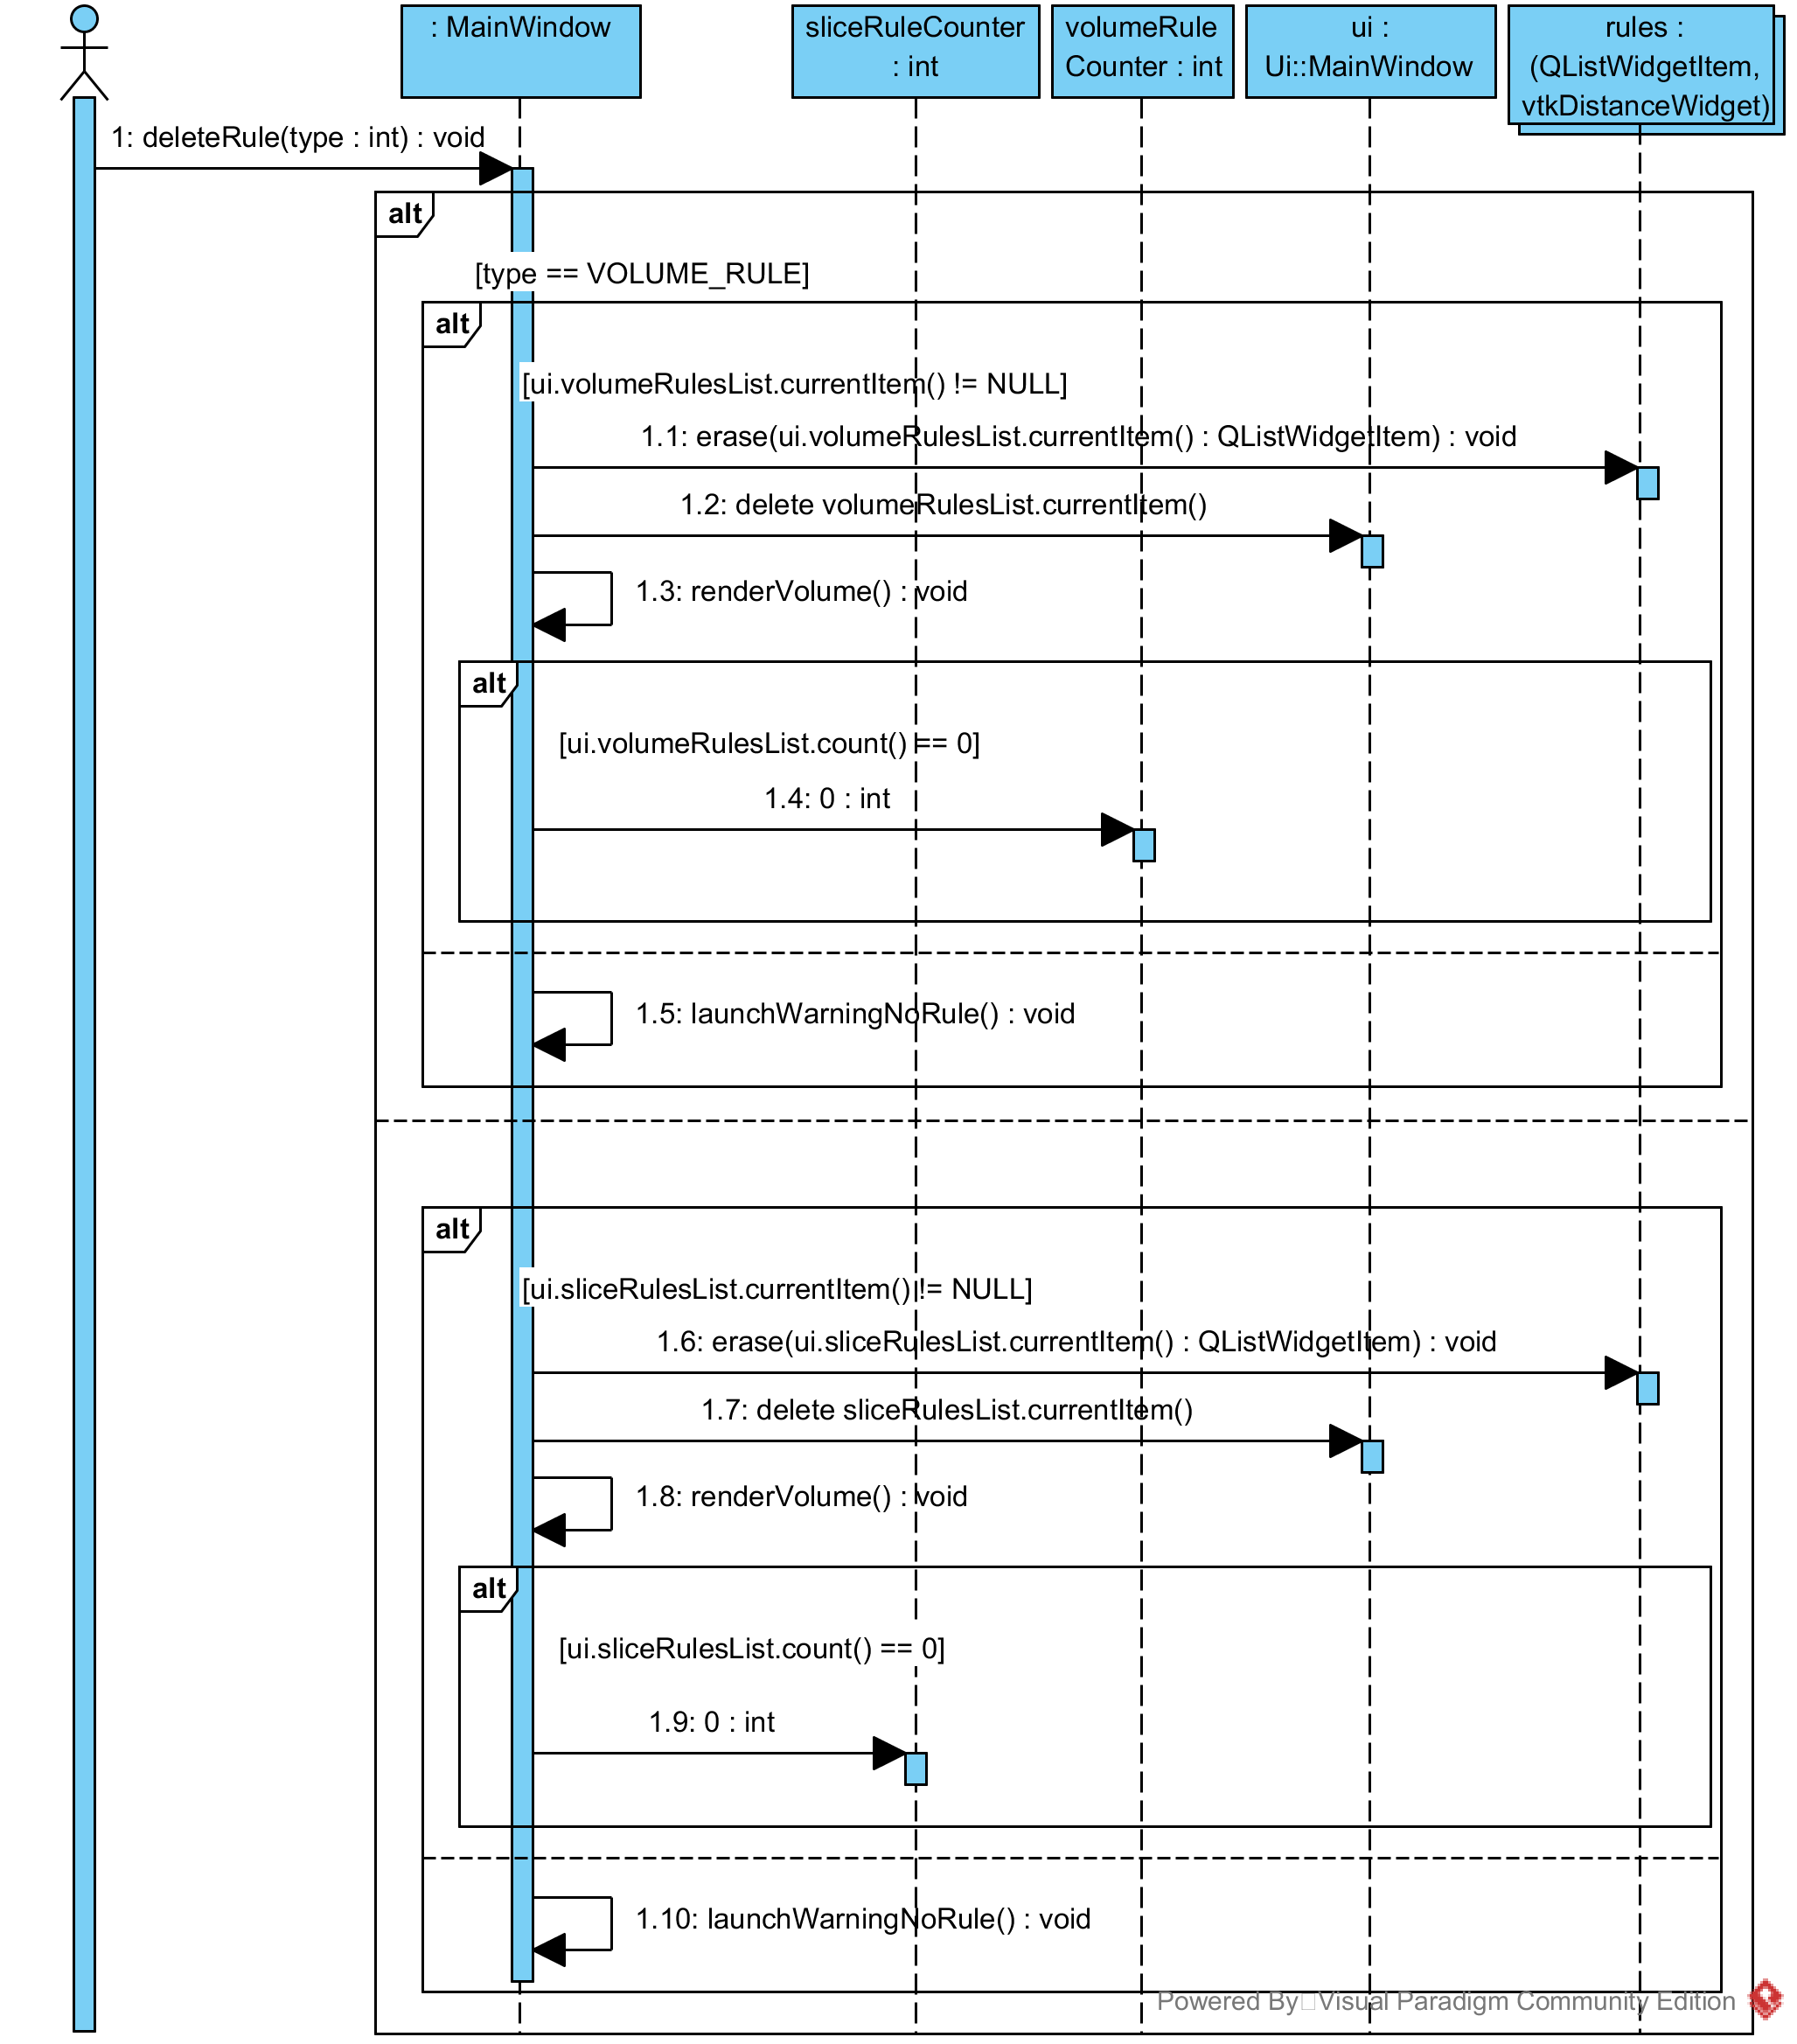
\includegraphics[width=12cm]{imagenes/diagramas/secuencia/MainWindow_DeleteRule}
	\caption{Diagrama de secuencia del método \textit{deleteRule} de \textit{MainWindow}}
	\label{fig:diagrama_secuencia_mainwindow_deleterule}
\end{figure}

\begin{figure}[H]
	\centering
	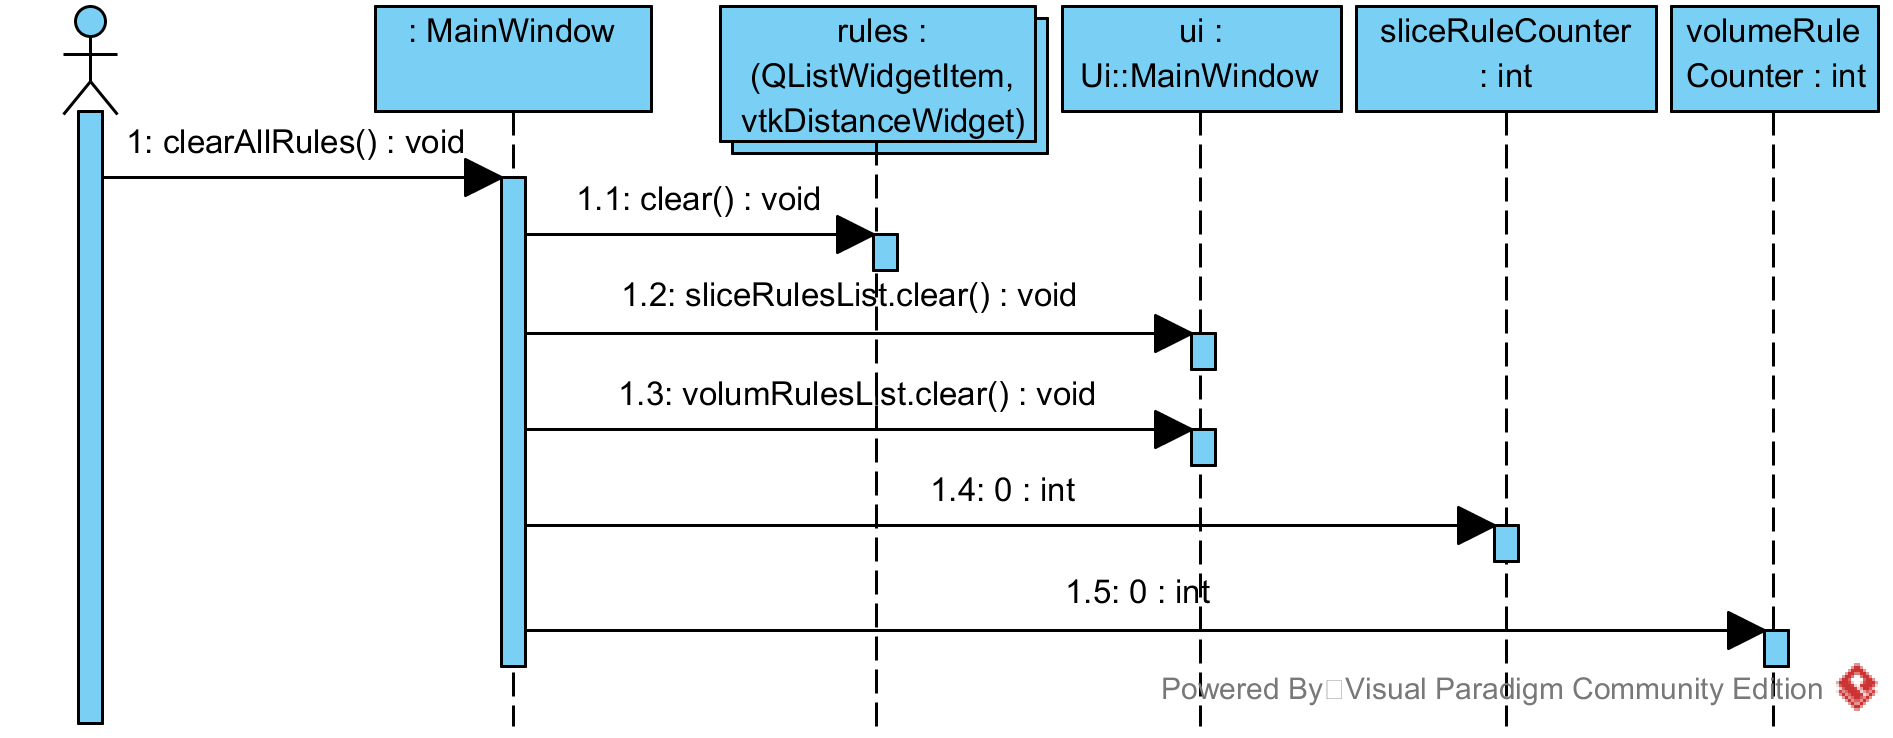
\includegraphics[width=12cm]{imagenes/diagramas/secuencia/MainWindow_ClearAllRules}
	\caption{Diagrama de secuencia del método \textit{clearAllRules} de \textit{MainWindow}}
	\label{fig:diagrama_secuencia_mainwindow_clearallrules}
\end{figure}

\subsection{InteractorStyleDeleter}

\begin{figure}[H]
	\centering
	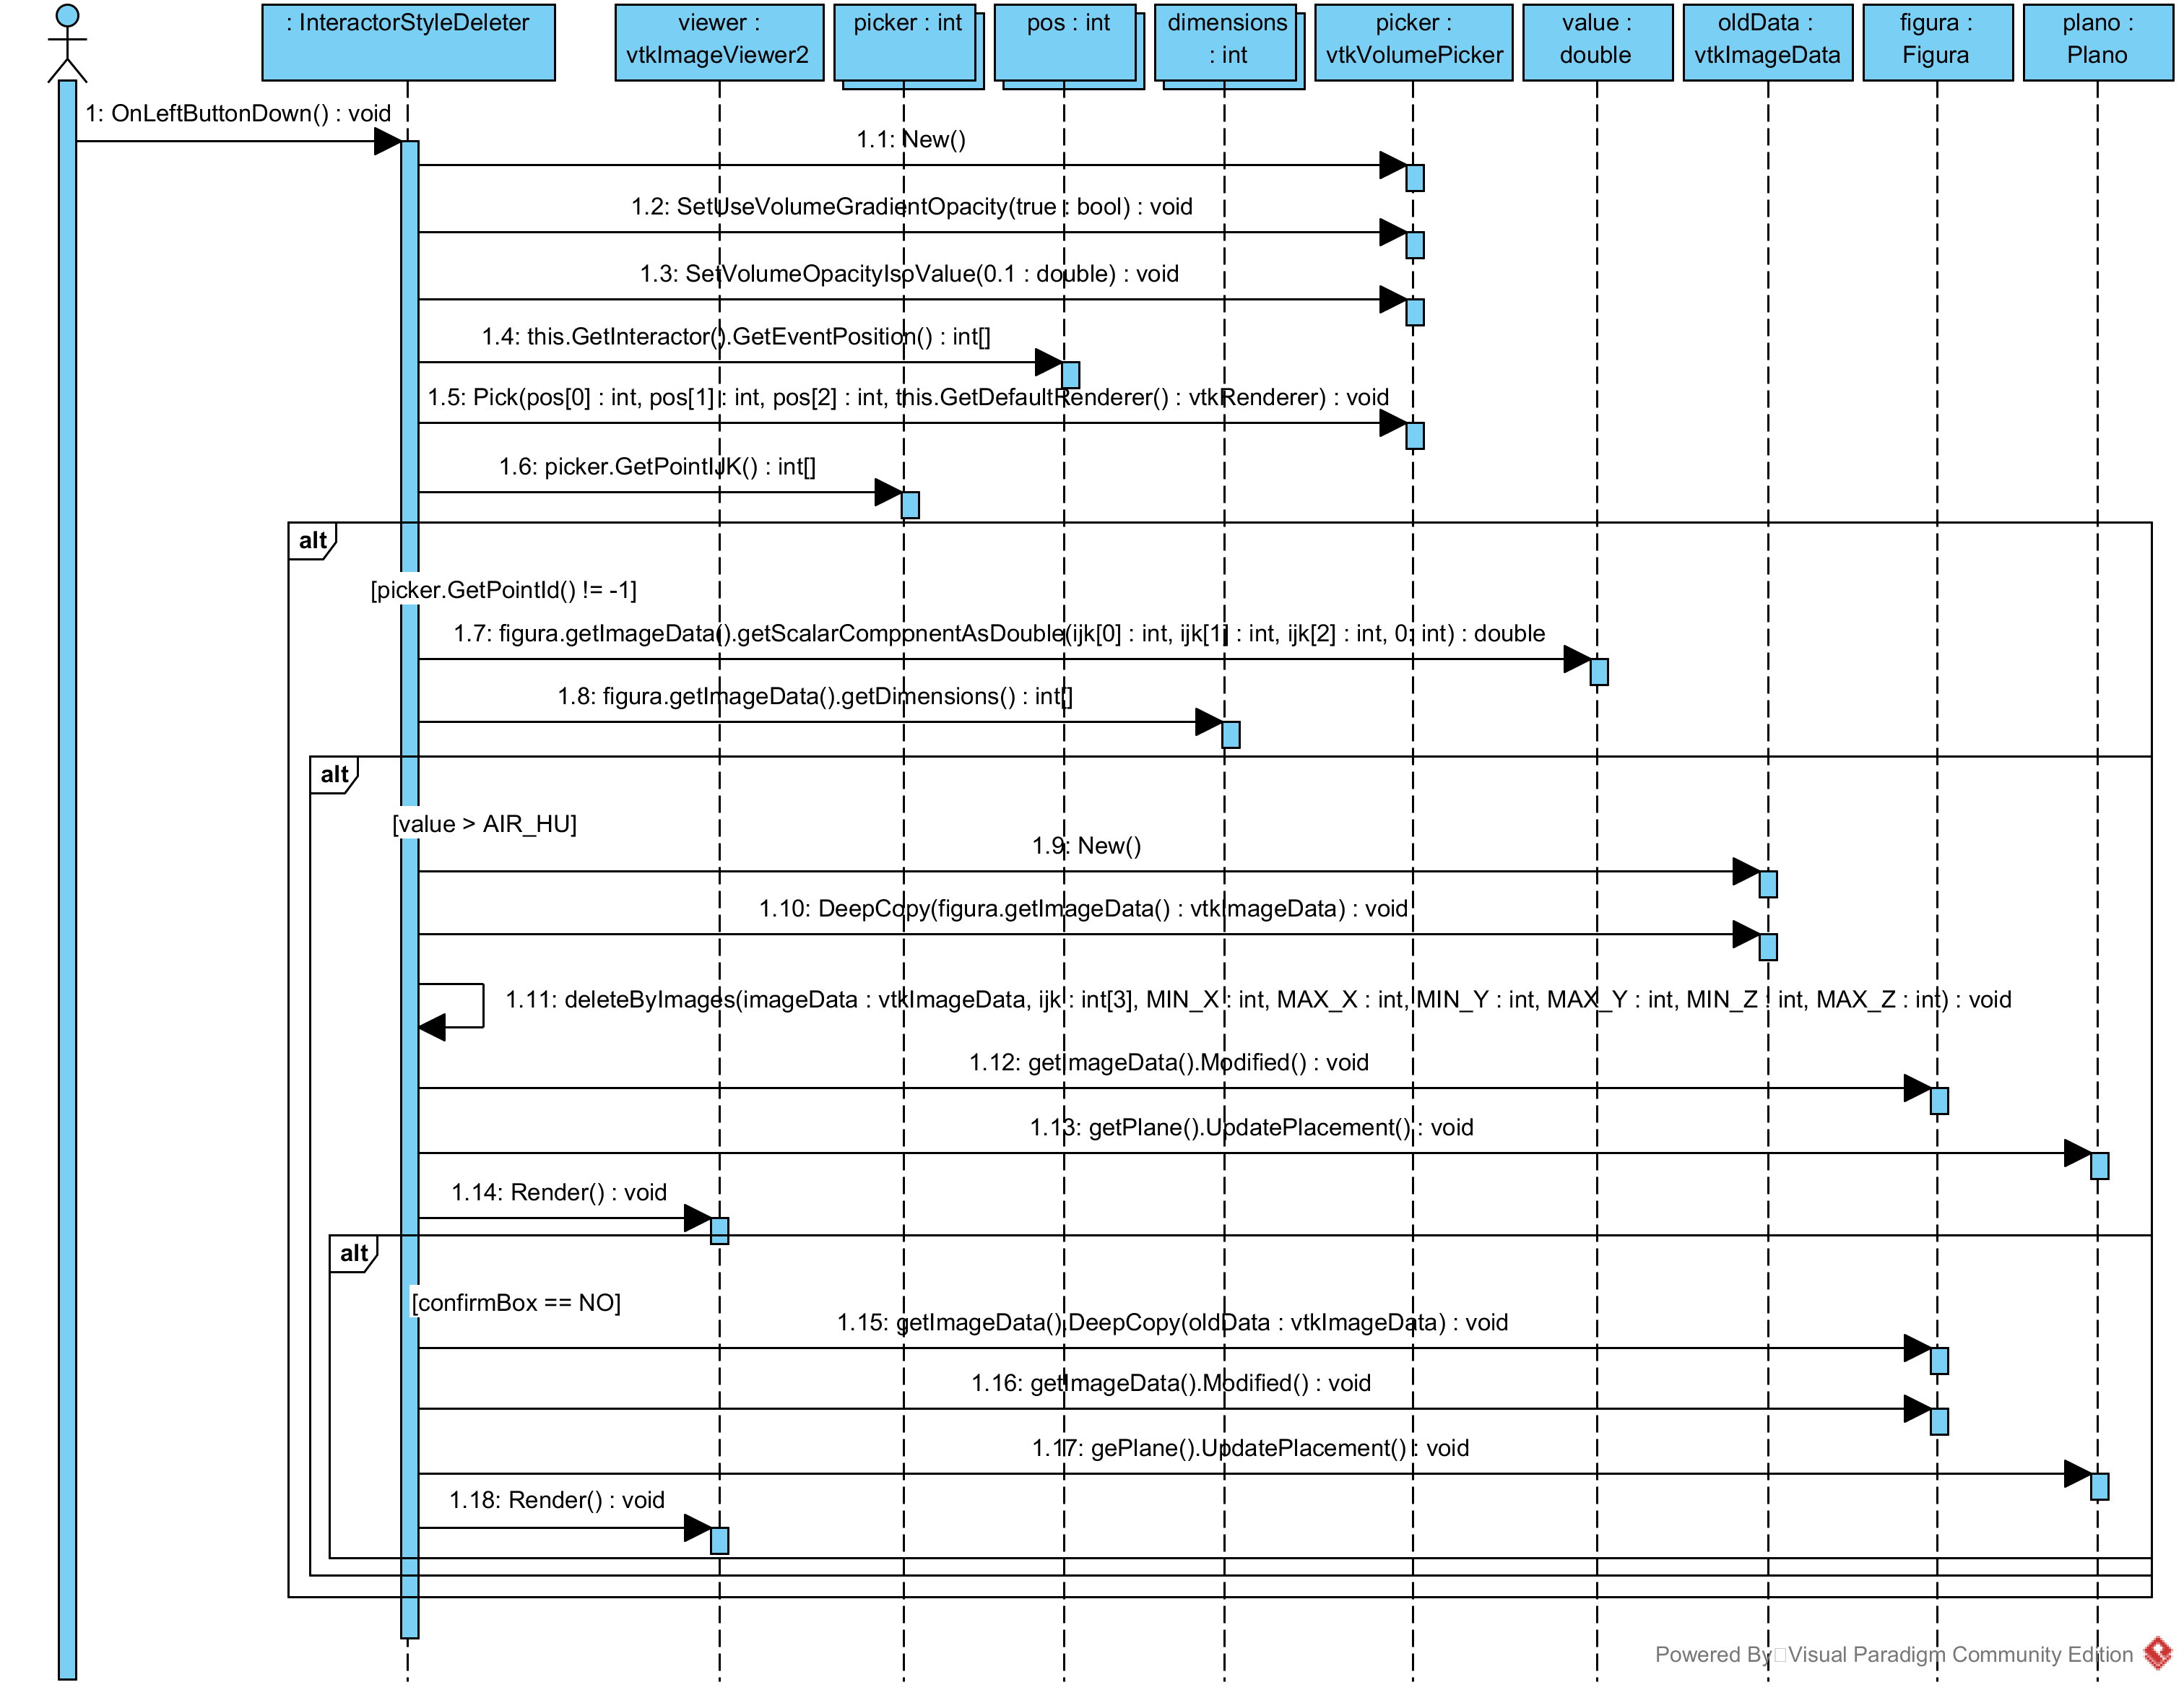
\includegraphics[angle=90,width=12cm]{imagenes/diagramas/secuencia/InteractorStyleDeleter_OnLeftButtonDown}
	\caption{Diagrama de secuencia del método \textit{OnLeftButtonDown} de \textit{InteractorStyleDeleter}}
	\label{fig:diagrama_secuencia_interactorstyledeleter_onfeftbuttondown}
\end{figure}

\begin{figure}[H]
	\centering
	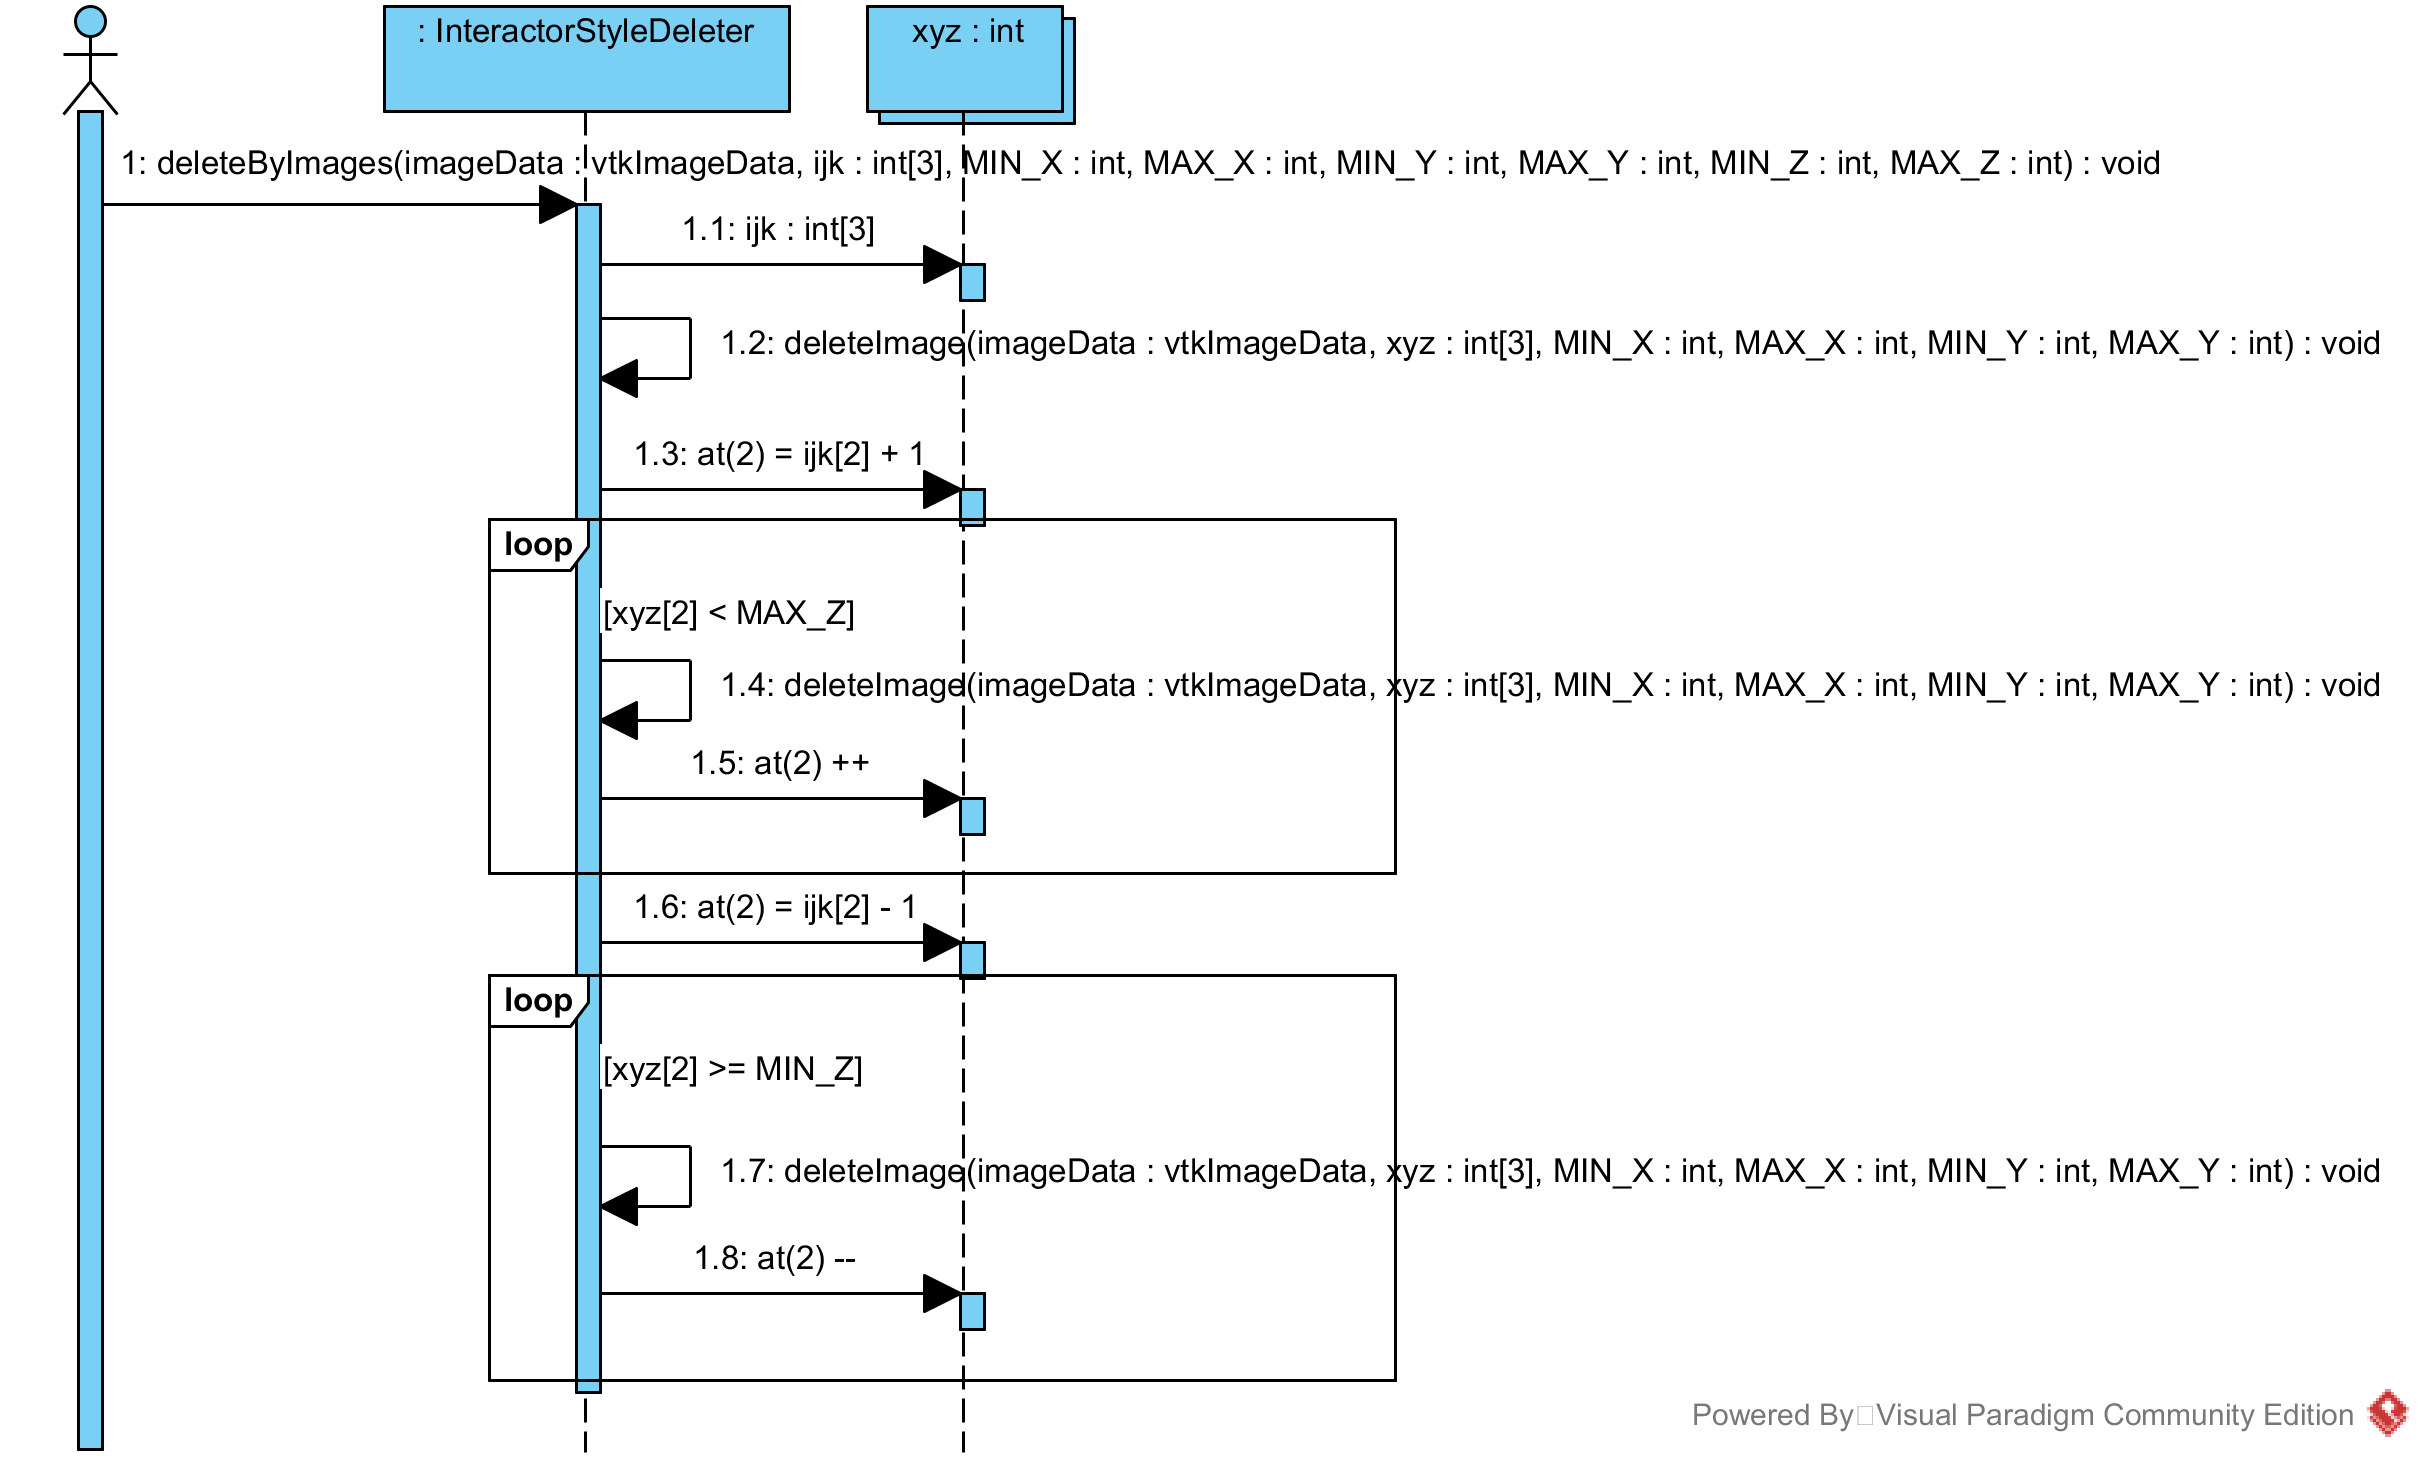
\includegraphics[angle=90,height=18cm]{imagenes/diagramas/secuencia/InteractorStyleDeleter_DeleteByImages}
	\caption{Diagrama de secuencia del método \textit{deleteByImages} de \textit{InteractorStyleDeleter}}
	\label{fig:diagrama_secuencia_interactorstyledeleter_deletebyimages}
\end{figure}

\begin{figure}[H]
	\centering
	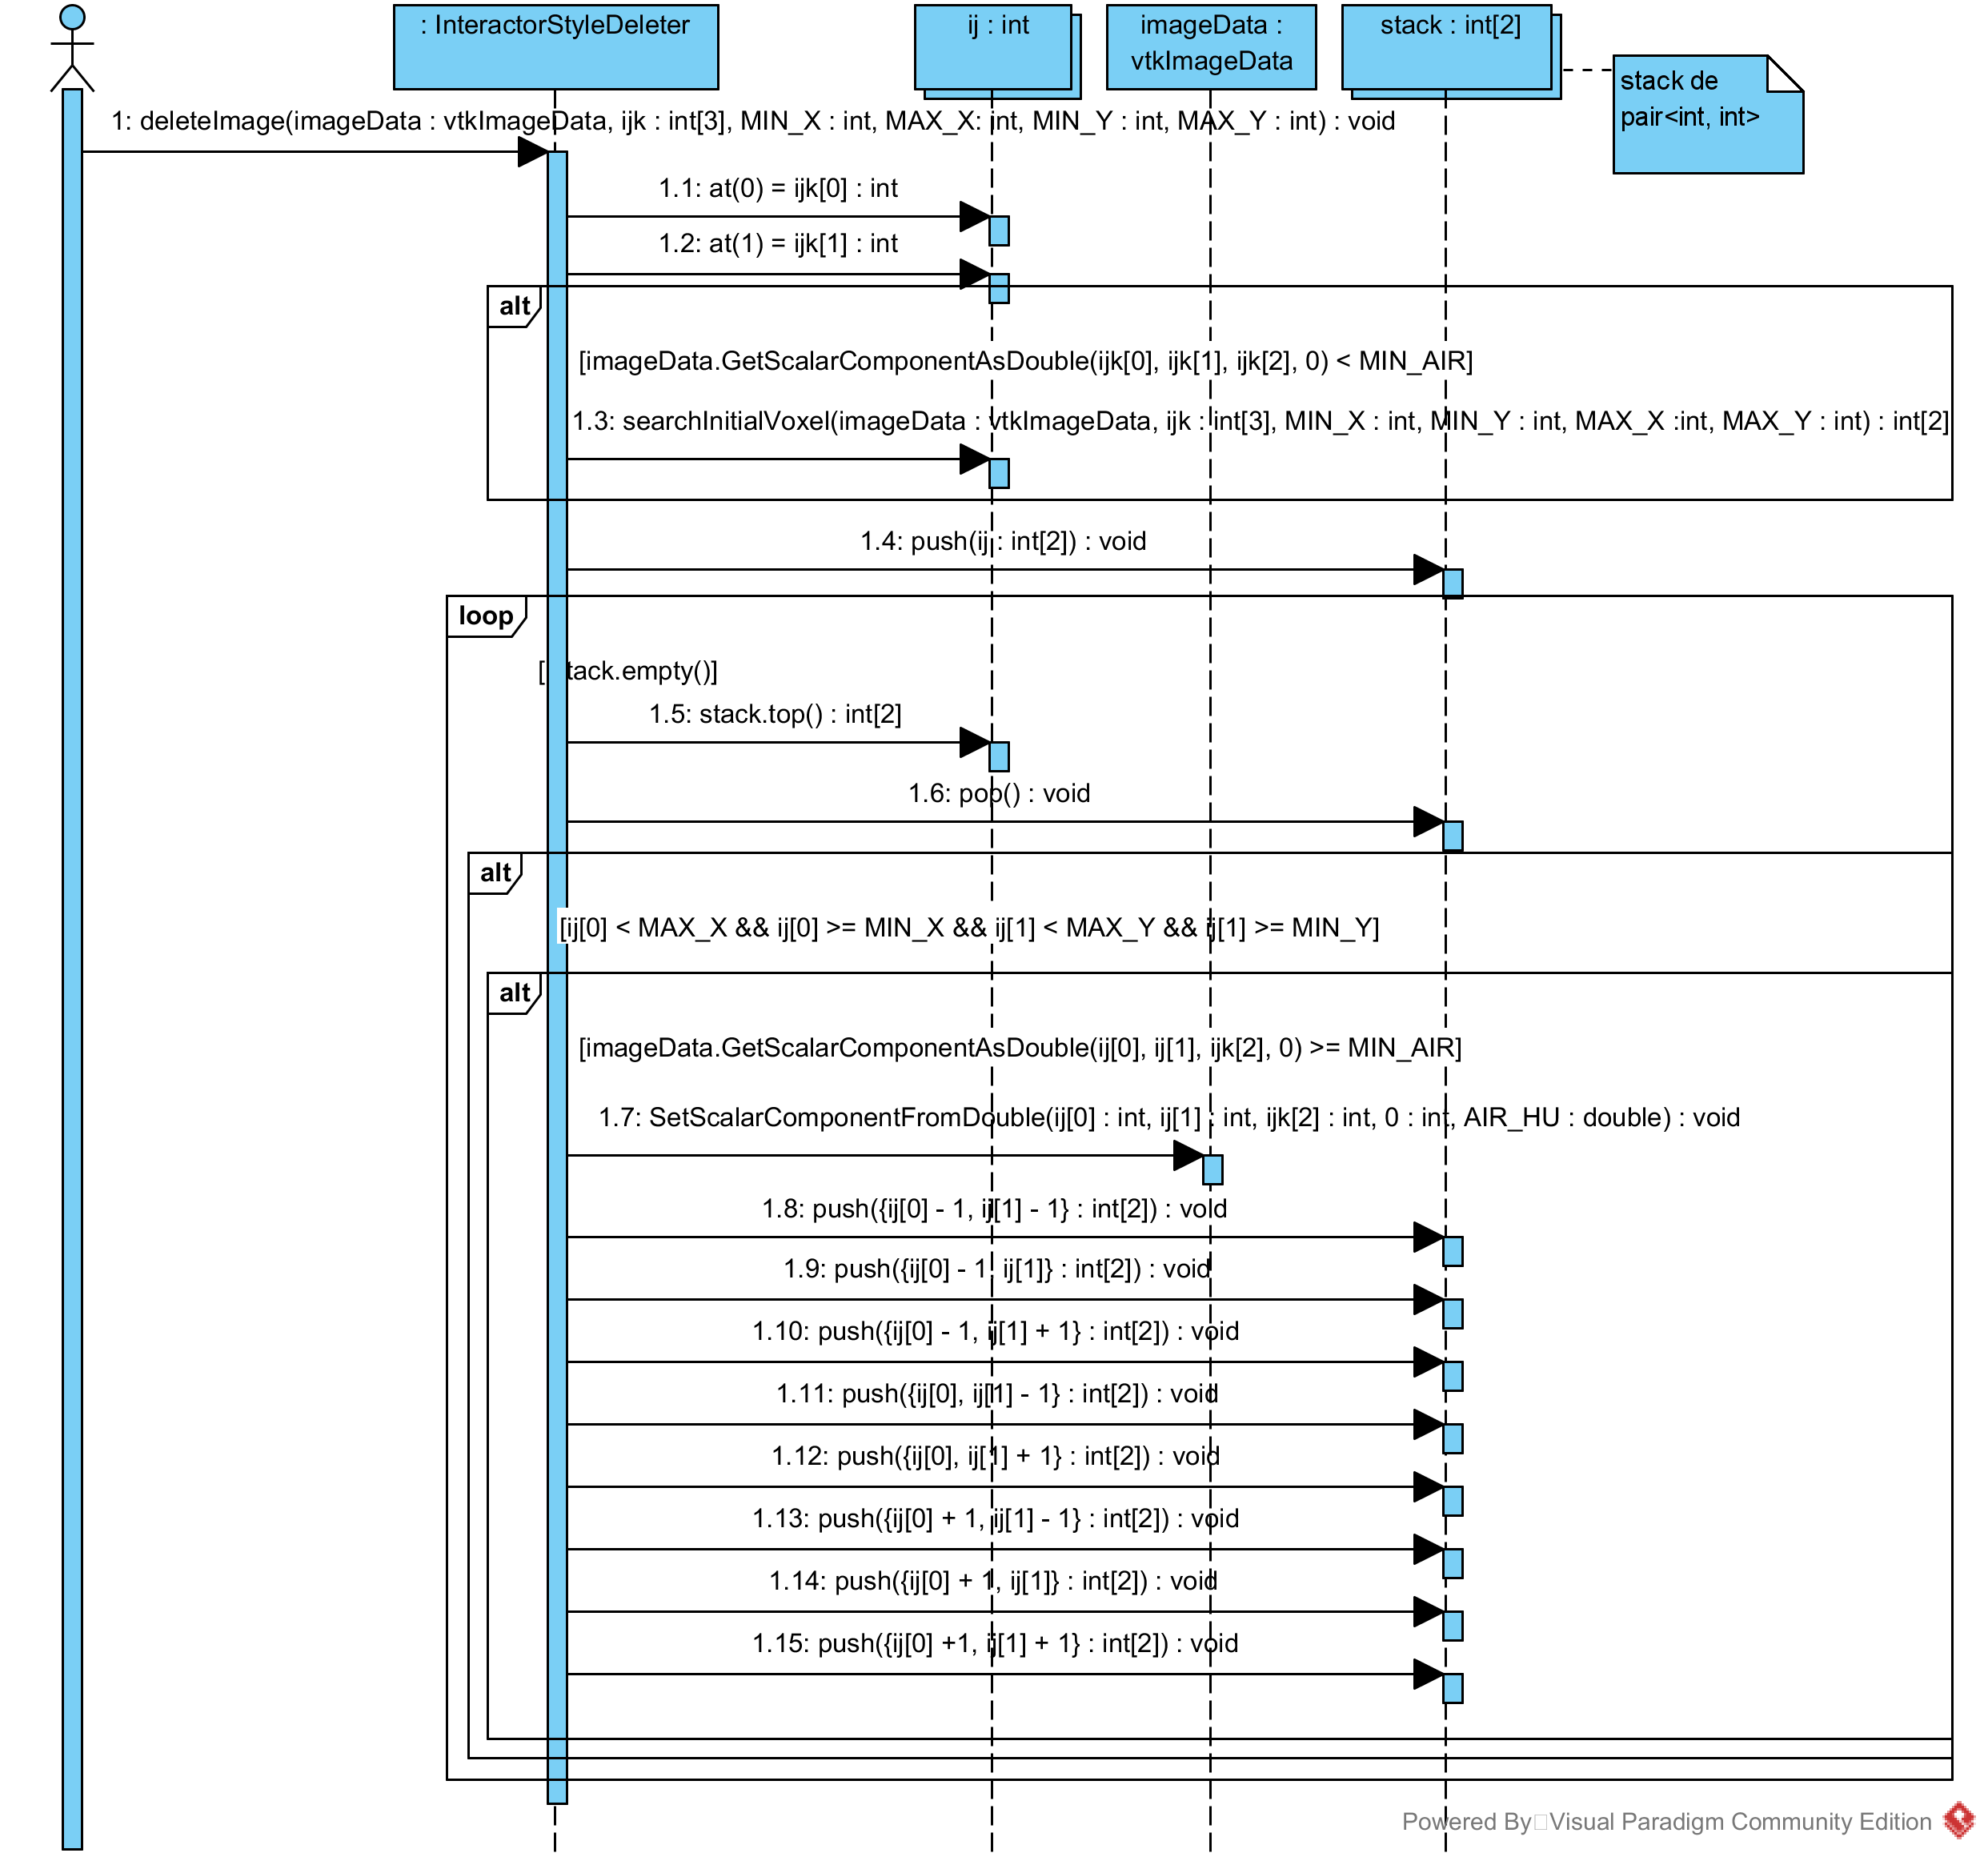
\includegraphics[width=12cm]{imagenes/diagramas/secuencia/InteractorStyleDeleter_DeleteImage}
	\caption{Diagrama de secuencia del método \textit{deleteImage} de \textit{InteractorStyleDeleter}}
	\label{fig:diagrama_secuencia_interactorstyledeleter_deleteimage}
\end{figure}

\begin{figure}[H]
	\centering
	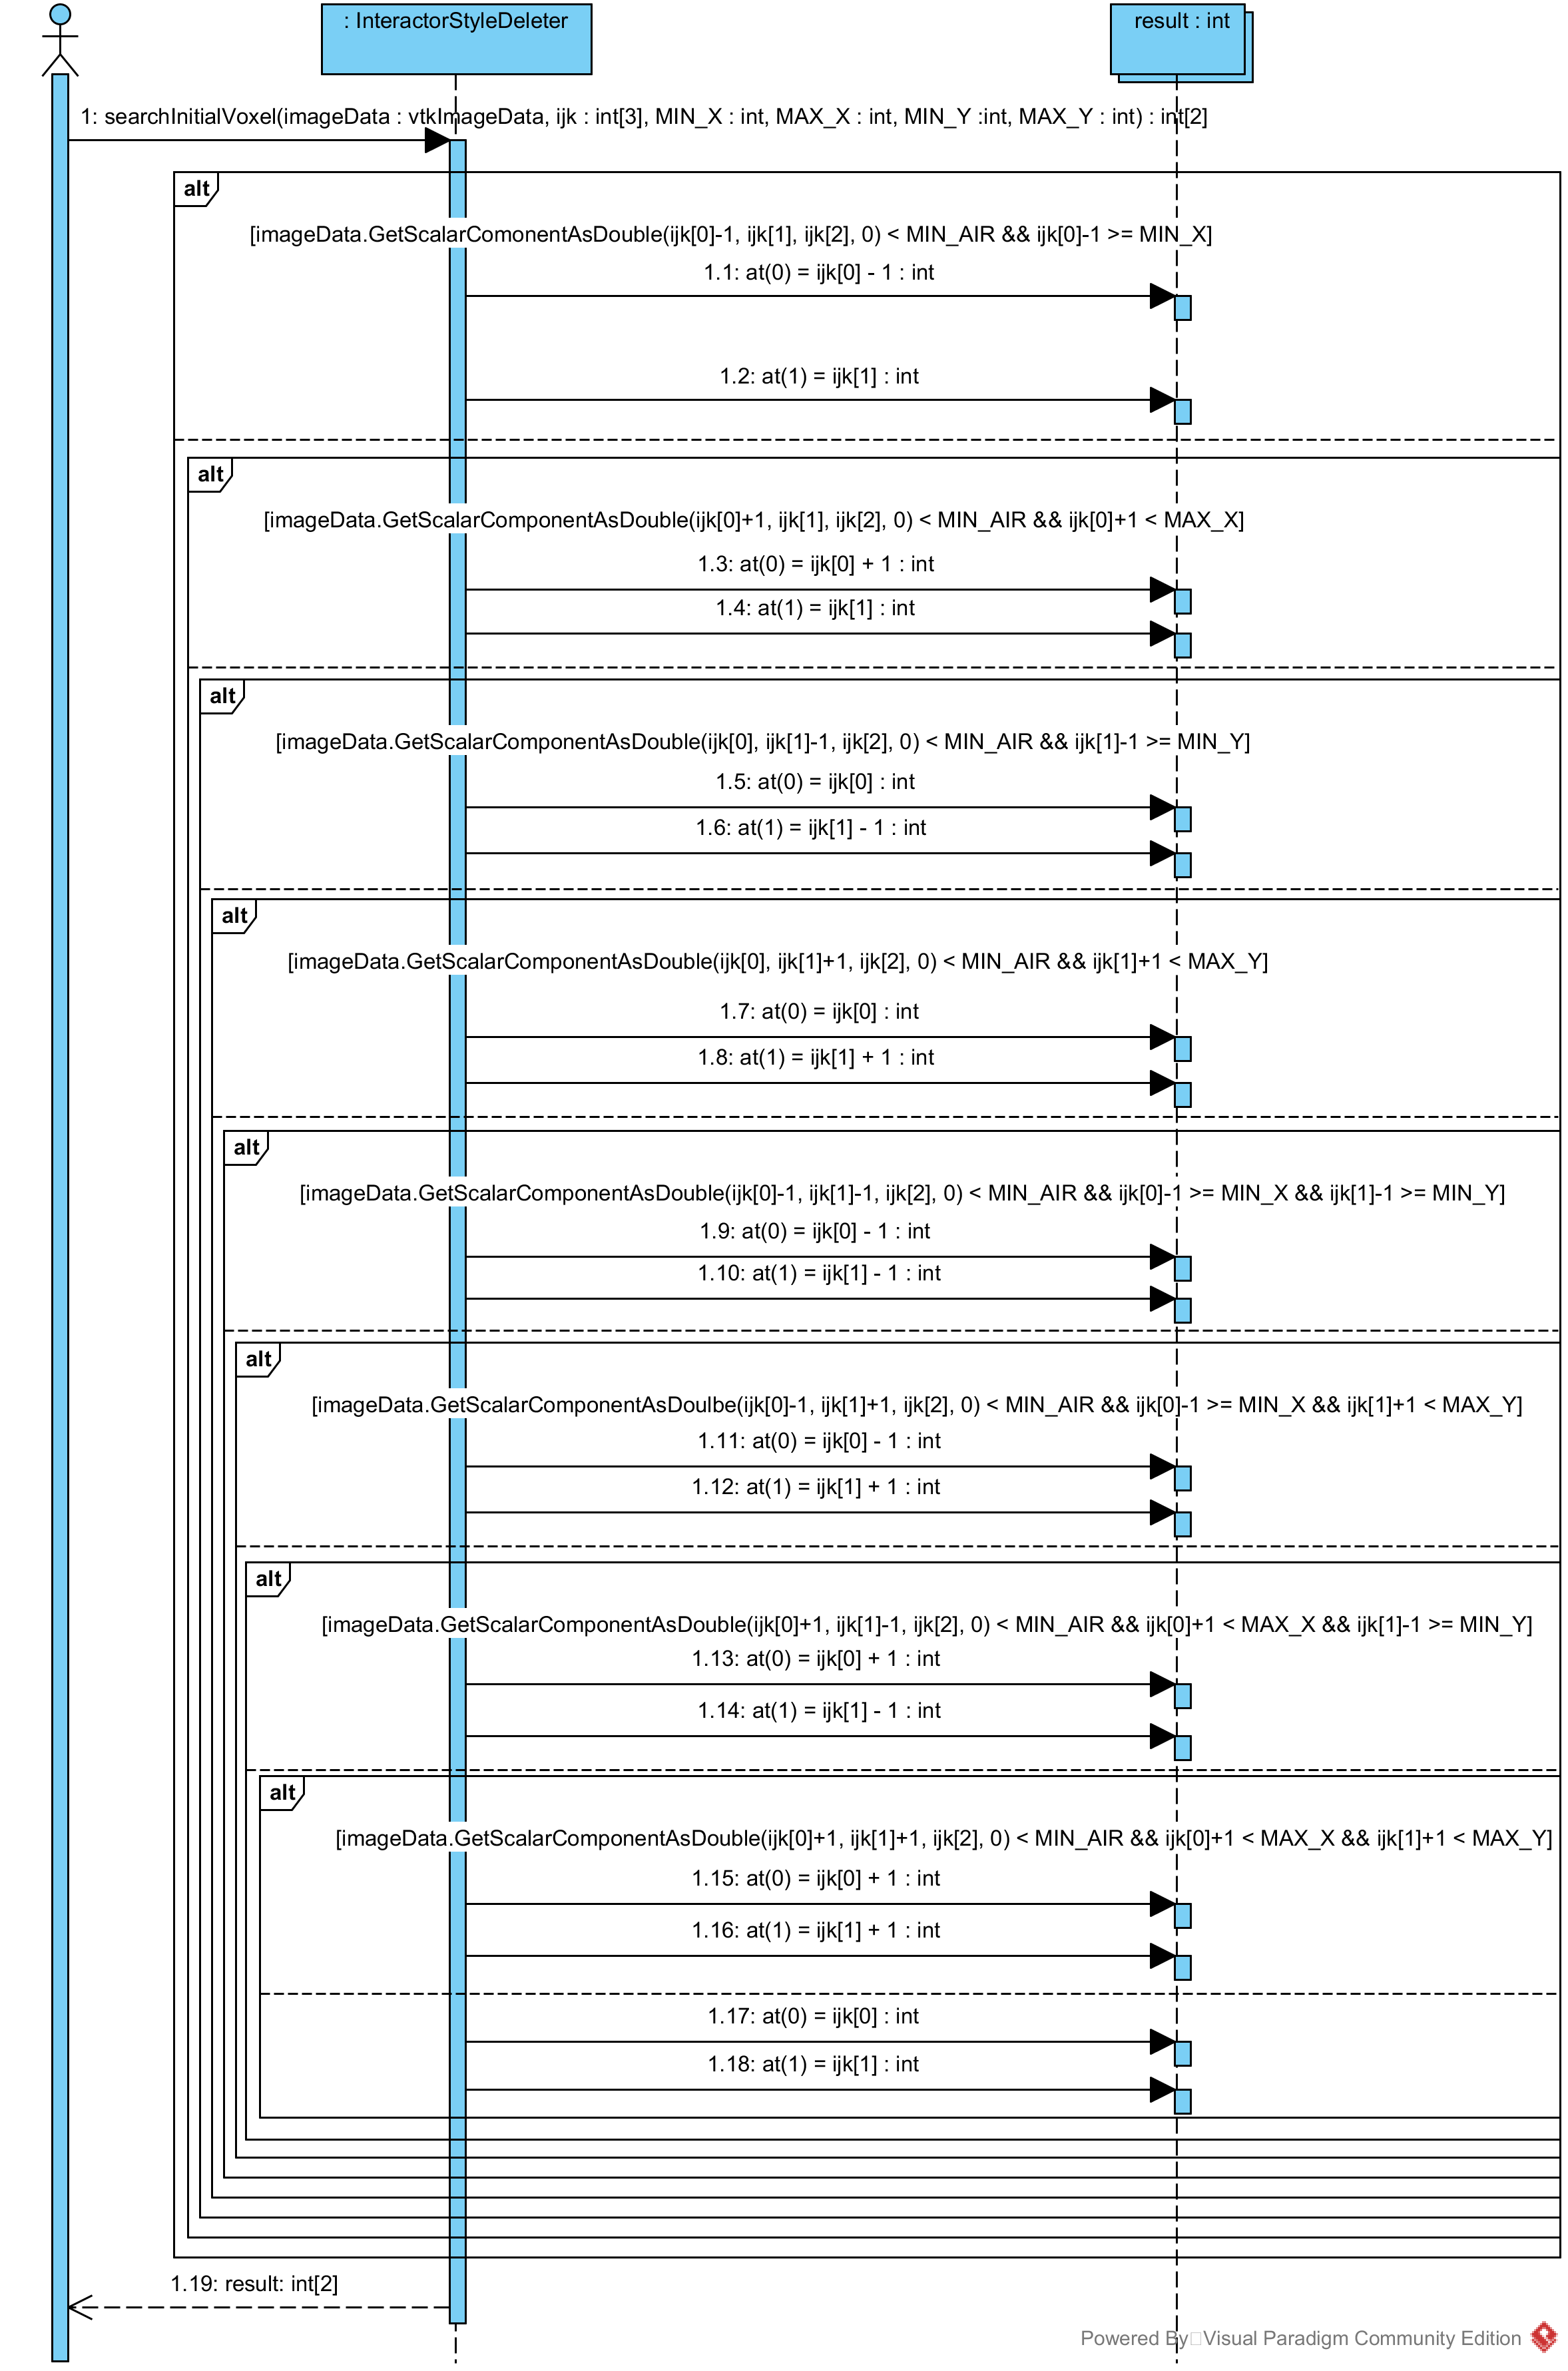
\includegraphics[width=12cm]{imagenes/diagramas/secuencia/InteractorStyleDeleter_SearchInitialVoxel}
	\caption{Diagrama de secuencia del método \textit{searchInitialVoxel} de \textit{InteractorStyleDeleter}}
	\label{fig:diagrama_secuencia_interactorstyledeleter_searchinitialvoxel}
\end{figure}

\subsection{InteractorStyleImage}

\begin{figure}[H]
	\centering
	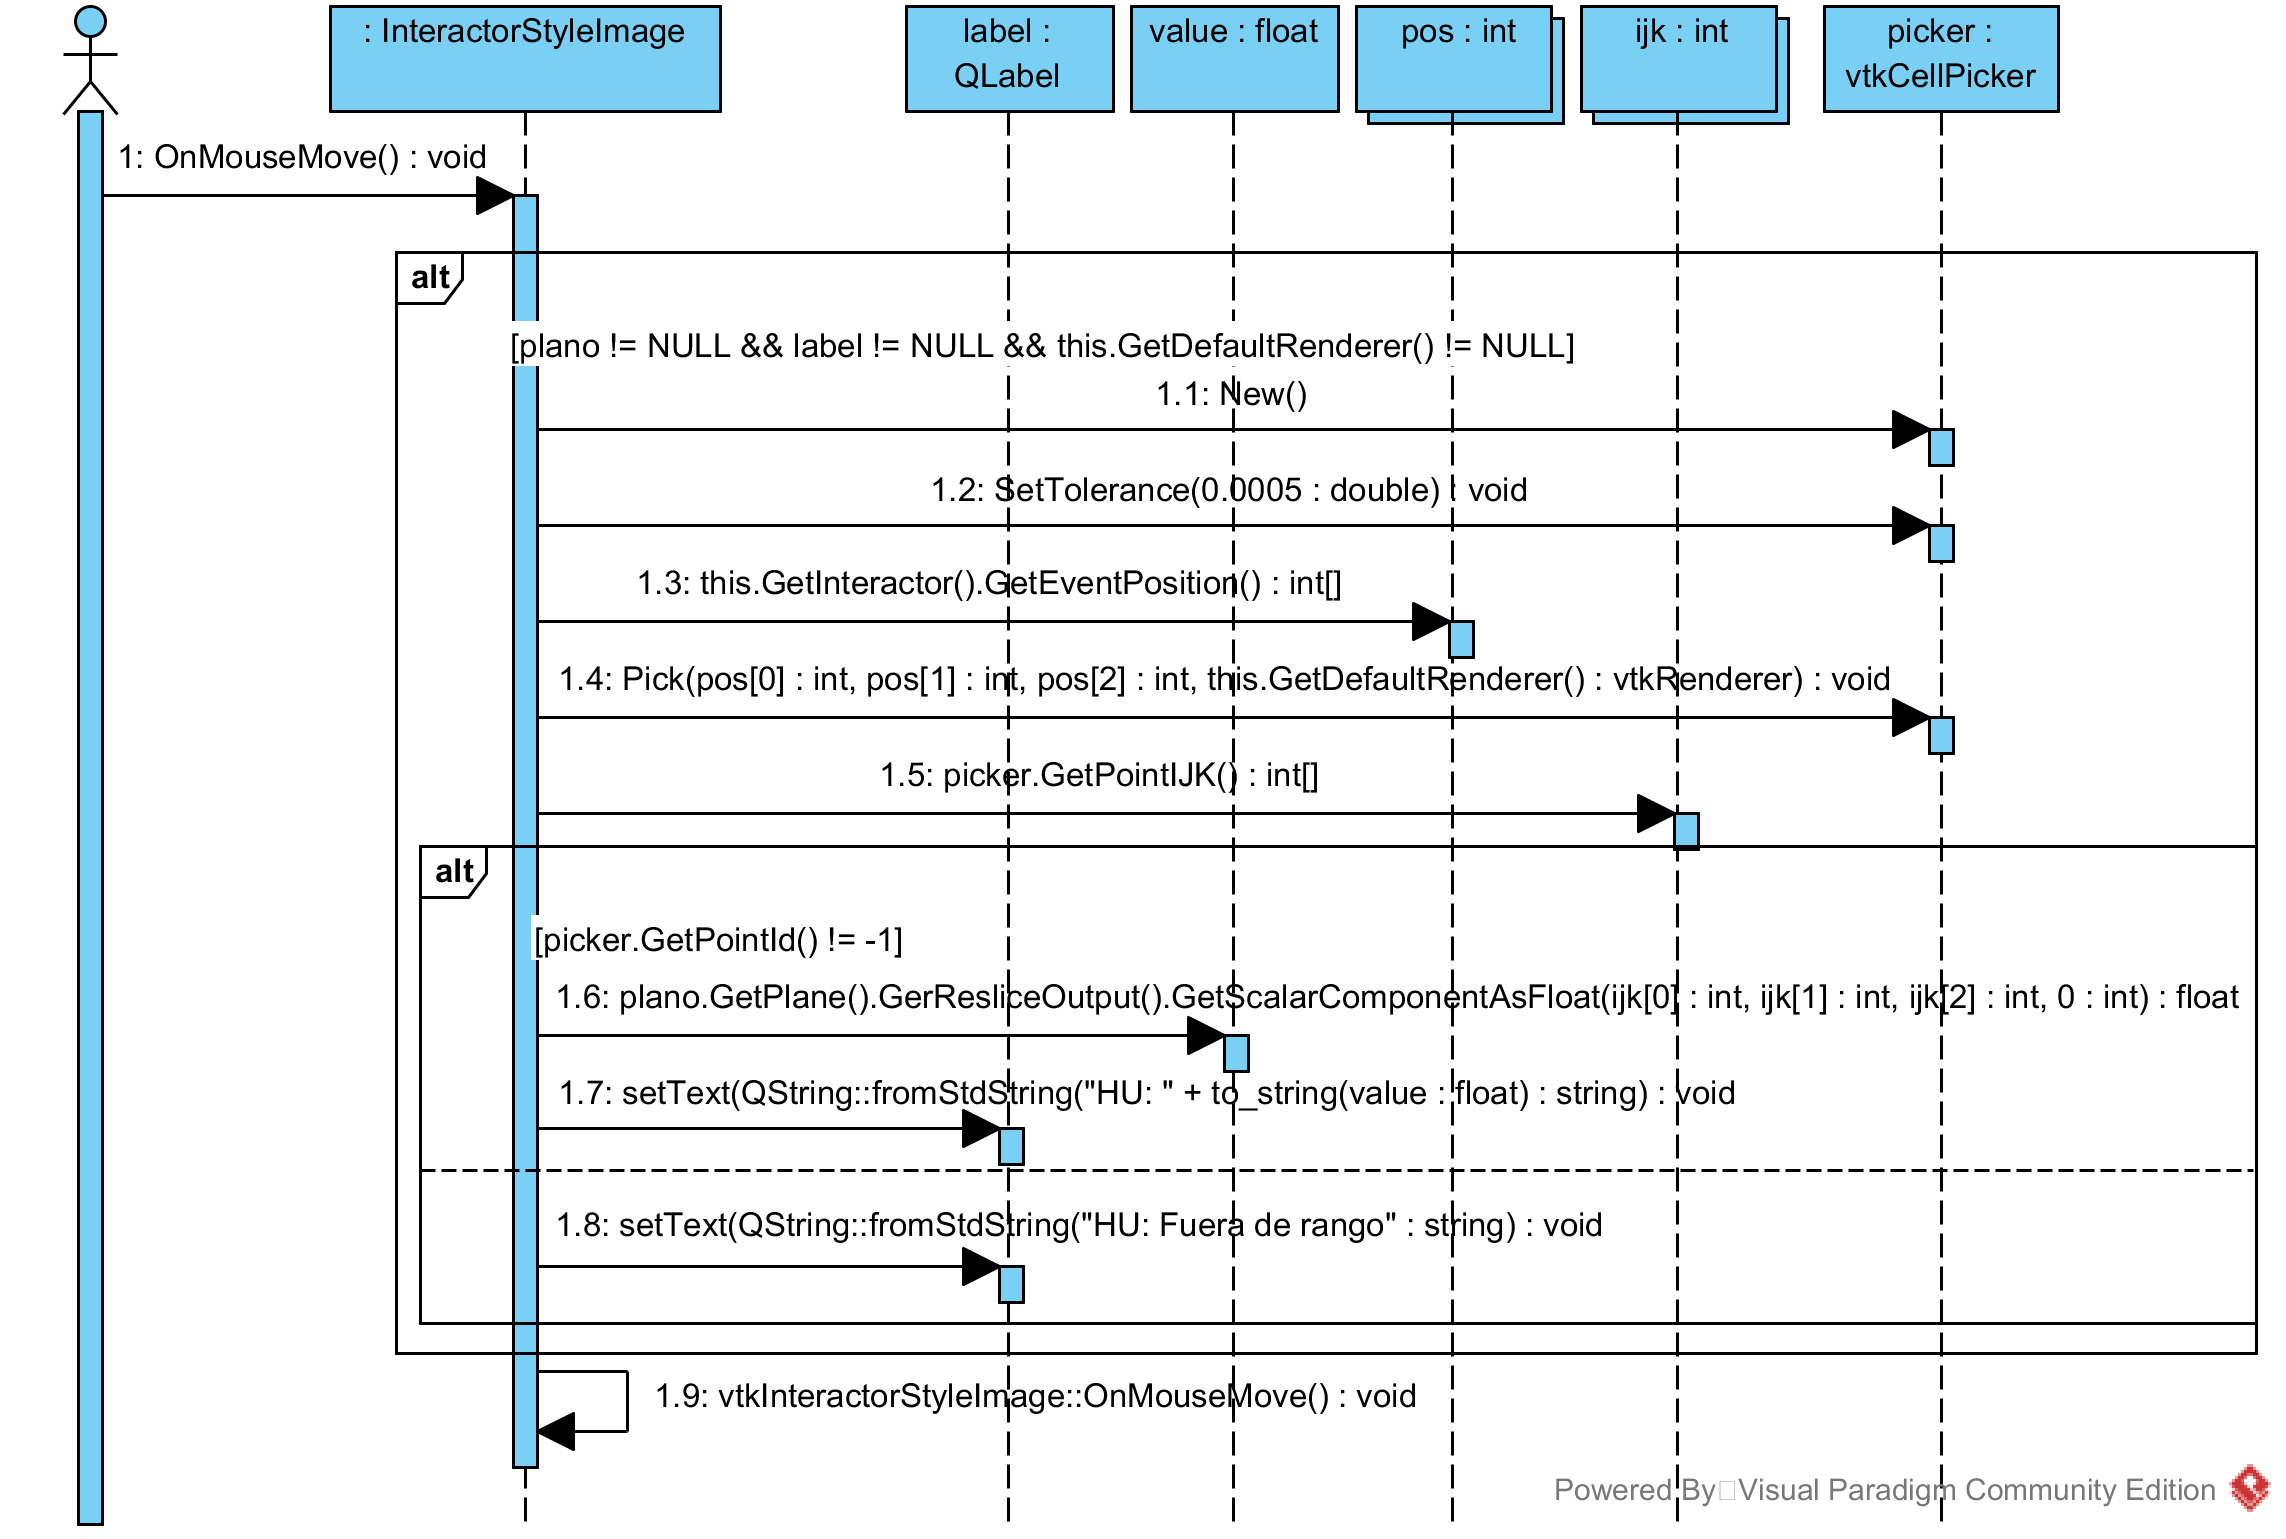
\includegraphics[angle=90,height=18cm]{imagenes/diagramas/secuencia/InteractorStyleImage_OnMouseMove}
	\caption{Diagrama de secuencia del método \textit{OnMouseMove} de \textit{InteractorStyleImage}}
	\label{fig:diagrama_secuencia_interactorstyleimage_onmousemove}
\end{figure}